\documentclass[lang=cn,newtx,10pt,scheme=chinese]{elegantbook}

\title{含参变量积分}
\subtitle{复习整理笔记}

\author{阮炜挺}
\institute{宁波大学数学与统计学院}
\date{}

\extrainfo{Given yourself an epsilon of room!}

\setcounter{tocdepth}{3}

\cover{cover.jpg}

% 本文档命令
\usepackage{array}
\newcommand{\ccr}[1]{\makecell{{\color{#1}\rule{1cm}{1cm}}}}

% 修改标题页的橙色带
\definecolor{customcolor}{RGB}{32,178,170}
\colorlet{coverlinecolor}{customcolor}
\usepackage{cprotect}

\addbibresource[location=local]{reference.bib} % 参考文献,不要删除
\everymath{\displaystyle} % 使所有公式默认使用行间公式
\usepackage{extarrows}

\begin{document}

\maketitle
\frontmatter

\tableofcontents

\mainmatter

\chapter{含参变量积分}

\section{基本定理}

\begin{theorem}[连续性]
设 $f(x,t)$ 在 $[a,b] \times [c,d]$ 上连续, 则 $\varphi(t) = \int_{a}^{b} f(x,t) dx$ 在 $[c,d]$ 上连续, 即
$$ \lim\limits_{t \to t_0} \int_{a}^{b} f(x,t) dx = \int_{a}^{b} f(x, t_0) dx = \int_{a}^{b} \lim\limits_{t \to t_0} f(x,t) dx, \quad \forall t_0 \in [c,d]. $$
\end{theorem}

\begin{theorem}[交换积分次序]
设 $f(x,t)$ 在 $[a,b] \times [c,d]$ 上连续, 则
$$ \int_{c}^{d} dt \int_{a}^{b} f(x,t) dx = \int_{a}^{b} dx \int_{c}^{d} f(x,t) dt. $$
\end{theorem}

\begin{theorem}[可微性]
设 $f(x,t), f_t(x,t)$ 在 $[a,b] \times [c,d]$ 上连续, 则 $\varphi(t) = \int_{a}^{b} f(x,t) dx$ 在 $[c,d]$ 上可导, 且
$$ \varphi'(t) = \int_{a}^{b} f_t(x,t) dx. $$
\end{theorem}

\begin{theorem}[一般情形的连续性与可微性]
设 $f(x,t)$ 在 $[a,b] \times [c,d]$ 上连续, 函数 $\alpha(t), \beta(t)$ 在 $[c,d]$ 上连续, 且 $a \le \alpha(t), \beta(t) \le b, \forall t \in [a,b]$, 则 $\varphi(t) = \int_{\alpha(t)}^{\beta(t)} f(x,t) dx$ 在 $[c,d]$ 上连续. 进一步, 若 $f_t(x,t)$ 在 $[a,b] \times [c,d]$ 上连续, $\alpha(t), \beta(t)$ 在 $[c,d]$ 上可导, 则 $\varphi(t)$ 也在 $[c,d]$ 上可导, 且
$$ \varphi'(t) = f[\beta(t),t]\beta'(t) - f[\alpha(t),t]\alpha'(t) + \int_{\alpha(t)}^{\beta(t)} f_t(x,t) dx. $$
\end{theorem}

\section{含参变量正常积分}

\subsection{简单例题}
\begin{example}
设 $f(x,y) = \operatorname{sgn}(x-y)$, 证明: 含参量积分 $F(y) = \int_{0}^{1} f(x,y) \,dx$ 在 $(-\infty, +\infty)$ 上连续.
\end{example}
\begin{solution}
对$y$的范围进行讨论有$F(y) = \begin{cases} 1, & y < 0, \\ 1-2y, & 0 \le y \le 1, \\ -1, & y > 1. \end{cases} $ $\blacksquare$
\end{solution} 

\begin{example}
设 $x>0$, 且 $f(x) = \int_{x}^{x^2} \frac{\sin ux}{u} \,du$, 求 $f'(x)$.
\end{example}
\begin{solution}
\begin{align*}
f'(x) &= 2x \cdot \frac{\sin x^3}{x^2} - \frac{\sin x^2}{x} + \int_{x}^{x^2} \cos ux \,du = \frac{2\sin x^3 - \sin x^2}{x} + \frac{\sin ux}{x} \bigg|_{x}^{x^2} = \frac{3\sin x^3 - 2\sin x^2}{x}. \blacksquare
\end{align*}

\end{solution}

\begin{example}[$\bigstar$]
设 $f(x)$ 在 $[0,1]$ 上连续, 讨论函数 $F(t) = \int_0^1 \frac{t}{x^2+t^2}f(x)dx$ 的连续性.
\end{example}

\begin{solution}
令 $g(x,t) = \frac{t}{x^2+t^2}f(x)$, 那么 $F(t) = \int_0^1 g(x,t) dx$. 注意到 $F(t)$ 是奇函数.
$\forall t_0 \in (0, +\infty)$, $g(x,t)$ 在 $[0,1] \times [\frac{t_0}{2}, 2t_0]$ 中连续, 那么 $F(t)$ 在 $[\frac{t_0}{2}, 2t_0]$ 连续.
从而 $F(t)$ 在 $t_0$ 点连续, 从而 $F(t)$ 在 $(0, +\infty)$ 连续. 同理 $F(t)$ 在 $(-\infty, 0)$ 也连续, 故 $F(t)$ 在 $(-\infty, 0) \cup (0, +\infty)$ 连续.

接下来讨论 $t=0$ 处. 首先有 $F(0)=0$. 再考虑
$$ \lim\limits_{t \to 0^+} F(t) = \boxed{\lim\limits_{t \to 0^+} \int_0^1 \frac{t}{x^2+t^2}f(x)dx }$$
我们将积分拆分为两部分:
$$ \int_0^1 \frac{t}{x^2+t^2}f(x)dx = \int_0^{t^{\frac{1}{4}}} \frac{t}{x^2+t^2}f(x)dx + \int_{t^{\frac{1}{4}}}^1 \frac{t}{x^2+t^2}f(x)dx = I_1 + I_2 $$
\begin{enumerate}
    \item 对于 $I_1 = \int_0^{t^{\frac{1}{4}}} \frac{t}{x^2+t^2}f(x)dx$, 由积分中值定理, 存在 $\xi \in (0, t^{\frac{1}{4}})$, 使得
    $$ I_1 = f(\xi) \int_0^{t^{\frac{1}{4}}} \frac{t}{x^2+t^2}dx = f(\xi)\left[\arctan \frac{x}{t}\right]_0^{t^{\frac{1}{4}}} = f(\xi) \arctan\frac{t^{\frac{1}{4}}}{t} = f(\xi) \arctan\frac{1}{t^{\frac{3}{4}}} $$
    那么当 $t \to 0^+$ 时, $\xi \to 0$, $\arctan\frac{1}{t^{\frac{3}{4}}} \to \frac{\pi}{2}$.
    从而
    $$ \lim\limits_{t \to 0^+} I_1 = \lim\limits_{t \to 0^+} f(\xi) \arctan\frac{1}{t^{\frac{3}{4}}} = f(0) \cdot \frac{\pi}{2} $$
    \item 对于 $I_2 = \int_{t^{\frac{1}{4}}}^1 \frac{t}{x^2+t^2}f(x)dx$, 由于 $f$ 在 $[0,1]$ 上连续, 故有界, 不妨设 $|f(x)| \le M$. 那么
    $$ |I_2| \le M \int_{t^{\frac{1}{4}}}^1 \frac{t}{x^2+t^2}dx = M \left(\arctan \frac{1}{t} - \arctan \frac{t^{\frac{1}{4}}}{t}\right) = M\left(\arctan\frac{1}{t} - \arctan\frac{1}{t^{\frac{3}{4}}}\right) $$
    由于当 $t \to 0^+$ 时, $\arctan\frac{1}{t} \to \frac{\pi}{2}$ 且 $\arctan\frac{1}{t^{\frac{3}{4}}} \to \frac{\pi}{2}$, 故 $\lim\limits_{t \to 0^+} M\left(\arctan\frac{1}{t} - \arctan\frac{1}{t^{\frac{3}{4}}}\right) = 0$.
    所以 $\lim\limits_{t \to 0^+} I_2 = 0$.
\end{enumerate}
由 1 和 2 可知 $\lim\limits_{t \to 0^+} F(t) = \frac{\pi}{2}f(0) + 0 = \frac{\pi}{2}f(0)$.
因为 $F(t)$ 是奇函数, 同理可得 $\lim\limits_{t \to 0^-} F(t) = -\lim\limits_{t \to 0^+} F(-t) = -F(0^+) = -\frac{\pi}{2}f(0)$.
$F(t)$ 在 $t=0$ 处连续的充要条件是左右极限存在且等于 $F(0)=0$.
$$ \lim\limits_{t \to 0^+} F(t) = \lim\limits_{t \to 0^-} F(t) = F(0) \implies \frac{\pi}{2}f(0) = -\frac{\pi}{2}f(0) = 0 $$
这等价于 $f(0)=0$.
所以, 当 $f(0)=0$ 时, $F(t)$ 在 $t=0$ 处连续. 当 $f(0) \neq 0$ 时, $F(t)$ 在 $t=0$ 处不连续.$\hfill \blacksquare$
\end{solution}

\begin{example}
证明函数 $J(x) = \frac{1}{\pi}\int_{0}^{\pi} \cos(t - x \sin t) \,dt$ 满足
$$ x^2 J''(x) + x J'(x) + (x^2 - 1)J(x) = 0. $$
\end{example}
\begin{note}
    操作过程中用分部积分把积分中的三角函数统一名称即可,需要注意的是分部积分过程中要看清楚是对哪个变量进行求导.此题也说明有时候通过简单的四则运算并不能消去所有项,这题最后剩下了一个积分为零的项.
\end{note}

\begin{solution}
首先注意到
\begin{align*}
J'(x) &= \frac{1}{\pi} \int_{0}^{\pi} \sin(t - x\sin t)\sin t \,dt = -\frac{1}{\pi} \int_{0}^{\pi} \sin(t - x\sin t) \,d(\cos t) \\
&= -\frac{1}{\pi}\sin(t-x\sin t)\cos t \bigg|_{0}^{\pi} + \frac{1}{\pi} \int_{0}^{\pi} \cos(t - x\sin t)(1 - x\cos t)\cos t \,dt  \text{\color{red}(注意分部积分的变量是t)}\\
&= \frac{1}{\pi} \int_{0}^{\pi} \cos(t-x\sin t)\cos t \,dt - \frac{x}{\pi}\int_{0}^{\pi} \cos(t-x\sin t)\cos^2 t \,dt.
\end{align*}
另外, 还有
\begin{align*}
J''(x) &= \frac{1}{\pi} \int_{0}^{\pi} \cos(t-x\sin t)(-\sin^2 t) \,dt \\
&= \frac{1}{\pi} \int_{0}^{\pi} \cos(t-x\sin t)\cos^2 t \,dt - \frac{1}{\pi}\int_{0}^{\pi} \cos(t-x\sin t) \,dt.
\end{align*}
由此可知
\begin{align*}
x^2 J''(x) + x J'(x) + (x^2-1)J(x) = -\frac{1}{\pi}\big[\sin(t-x\sin t)\big]_{0}^{\pi} = 0.\blacksquare
\end{align*}


\end{solution}

\begin{example}
设 $f(x)$ 在 $a$ 的某邻域内具有连续的 $n+1$ 阶导函数, 求 $\lim\limits_{x \to a} \frac{d^n}{dx^n} \left[ \frac{f(x) - f(a)}{x-a} \right]$.
\end{example}

\begin{solution}
注意到 $x \neq a$ 时, 有
$$ \boxed{\frac{f(x)-f(a)}{x-a} = \int_{0}^{1} f'(a+t(x-a)) \,dt}. $$
因此
$$ \frac{d^n}{dx^n} \left[ \frac{f(x)-f(a)}{x-a} \right] = \int_{0}^{1} f^{(n+1)}(a+t(x-a))\cdot t^n \,dt. $$
再结合 $f^{(n+1)}(x)$ 的\underline{连续性}, 有
$$ \lim\limits_{x \to a} \frac{d^n}{dx^n} \left[ \frac{f(x)-f(a)}{x-a} \right] = \int_{0}^{1} \lim\limits_{x \to a} \left\{ f^{(n+1)}[a+t(x-a)] \cdot t^n \right\} dt = f^{(n+1)}(a) \int_{0}^{1} t^n \,dt = \frac{f^{(n+1)}(a)}{n+1}. $$
\hfill $\blacksquare$
\end{solution}

\begin{example}
设 $F(t) = \int_{0}^{t} dx \int_{x^2}^{t^2} f(x,y) \,dy$, 其中 $f(x,y)$ 为连续函数, 求 $F'(t)$.
\end{example}

\begin{solution}
即定理1.4的应用.
记 $g(x,t) = \int_{x^2}^{t^2} f(x,y) \,dy$, 则 $F(t) = \int_{0}^{t} g(x,t) \,dx$,又因为$g_t(x,t) = f(x,t^2)\cdot 2t + \int_{x^2}^{t^2} f_t(x,y)dy = 2tf(x,t^2)$,
从而有$F'(t) = g(t,t)+\int_{0}^{t}g_t(x,t)dx = \int_{0}^{t}2tf(x,t^2)dx$ $blacksquare$.
\end{solution}
\begin{note}
    累次含参变量积分的处理方法,通过设 $g(x,t)$ 为积分的被积函数, 来化为一般形式的含参变量积分.
\end{note}

\begin{example}
设 $F(t) = \int_0^a dx \int_0^a f(x+y+t) dy$, 其中 $f$ 为连续函数. 证明
$$F''(t) = f(t+2a) - 2f(t+a) + f(t).$$
\end{example}

\begin{solution}
由于 $f$ 只是连续函数, 故不能直接对积分号下的 $f$ 求二阶导数.
令 $g(x,t) = \int_0^a f(x+y+t) dy$, 从而 $F(t) = \int_0^a g(x,t) dx$.
不妨设 $f$ 的原函数为 $H$, $H$ 的原函数为 $G$. (即 $H'=f, G'=H, G''=f$)
那么
$$ g(x,t) = \int_0^a f(x+y+t) dy = \big[ H(x+y+t) \big]_{y=0}^{y=a} = H(x+t+a) - H(x+t). $$
而
\begin{align*}
F(t) &= \int_0^a g(x,t) dx = \int_0^a [H(x+t+a) - H(x+t)] dx \\
&= \big[ G(x+t+a) \big]_{x=0}^{x=a} - \big[ G(x+t) \big]_{x=0}^{x=a} \\
&= [G(a+t+a) - G(0+t+a)] - [G(a+t) - G(0+t)] \\
&= G(t+2a) - G(t+a) - G(t+a) + G(t) \\
&= G(t+2a) - 2G(t+a) + G(t).
\end{align*}
那么
$$ F''(t) = \frac{d^2}{dt^2} [G(t+2a) - 2G(t+a) + G(t)] = G''(t+2a) - 2G''(t+a) + G''(t). $$
因为 $G''=f$, 所以
$$ F''(t) = f(t+2a) - 2f(t+a) + f(t) \blacksquare$$
\end{solution}

\begin{example}[$\bigstar$]
计算累次积分 $\int_0^1 dx \int_0^1 \frac{x^2 - y^2}{(x^2 + y^2)^2} dy$ 与  $\int_0^1 dy \int_0^1 \frac{x^2 - y^2}{(x^2 + y^2)^2} dx$.
\end{example}

\begin{solution}
    令$$P(x,y) = \frac{x}{(x^2 + y^2)}, Q(x,y) = \frac{y}{(x^2 + y^2)}$$ 注意到$$P_x(x,y) = \frac{y^2 - x^2}{(x^2 + y^2)^2}, Q_y(x,y) = \frac{x^2 - y^2}{(x^2 + y^2)^2}$$
    且有$-P_x(x,y) = Q_y(x,y)$

    那么
    $$
    \int_0^1 dx \int_0^1 \frac{x^2 - y^2}{(x^2 + y^2)^2} dy = \int_0^1 dx \int_0^1 Q_y(x,y) dy = \int_0^1 Q(x,y) \bigg|_{y=0}^{y=1} dx = \int_0^1 \frac{1}{1+x^2} dx = \frac{\pi}{4}.
    $$
    同理
    $$
    \int_0^1 dy \int_0^1 \frac{x^2 - y^2}{(x^2 + y^2)^2} dx = \int_0^1 dy \int_0^1 -P_x(x,y) dx = \int_0^1 -P(x,y) \bigg|_{x=0}^{x=1} dy = -\int_0^1 \frac{1}{1+y^2} dy = -\frac{\pi}{4}.
    $$
    $\hfill \blacksquare$
\end{solution}

\subsection{含参变量积分的计算}
\begin{proposition}
当 $|a|<1$ 时, 有
\begin{equation*}
\int \frac{dx}{1+a\cos x} = \frac{2}{\sqrt{1-a^2}} \arctan\left(\sqrt{\frac{1-a}{1+a}}\tan\frac{x}{2}\right) + C. 
\end{equation*}

特别地, 有
\begin{equation*}
\int_{0}^{\pi} \frac{dx}{1+a\cos x} = \frac{\pi}{\sqrt{1-a^2}}, \quad |a|<1. 
\end{equation*}
类似的还有
$$
\int_{0}^{\pi} \frac{1}{a + \cos x} dx = \frac{\pi}{\sqrt{a^2 - 1}}, \quad a > 1.
$$

$$
\int_{0}^{\pi} \frac{1}{a + \cos x} dx =  - \frac{\pi}{\sqrt{a^2 - 1}}, \quad a < 1.
$$
\end{proposition}
\begin{remark}
    此命题用万能公式即可.
\end{remark}

如果直接求$\varphi(t) = \int_{a}^{b}f(x,t) \mathrm d x$有困难,那么通常采用以下两种方法:
\textcolor{blue}{\begin{enumerate}
    \item \textbf{积分号下积分}:把$f(x,t)$表示为积分形式,再用积分号下求积分的方法,此时通常要交换积分次序,所以要先判断函数的连续性.
    \item \textbf{积分号下微分}:先求$\varphi'(t)$,即先求$\int_{a}^{b}f_t(x,t) \mathrm d x$,然后再对$t$积分求出$\varphi(t)$,所以要先判断$f(x,t)$和$f_t(x,t)$的连续性.
\end{enumerate}}

\subsubsection{积分号下积分}

\begin{example}
计算 $\int_0^1 \frac{x^b - x^a}{\ln x} dx$, 其中 $0 < a < b$.
\end{example}

\begin{solution}
注意到 $$\frac{x^b - x^a}{\ln x} = \left[ \frac{x^y}{\ln x} \right]_{y=a}^{y=b} = \int_a^b x^y dy$$
那么
\begin{align*}
\int_0^1 \frac{x^b - x^a}{\ln x} dx &= \int_0^1 dx \int_a^b x^y dy \quad (\text{由于 } x^y \text{ 在 } [0,1] \times [a,b] \text{ 上连续, 故可交换积分次序}) \\
&= \int_a^b dy \int_0^1 x^y dx = \int_a^b \left[ \frac{x^{y+1}}{y+1} \right]_{x=0}^{x=1} dy = \int_a^b \frac{1}{y+1} dy \\
&= \big[ \ln(y+1) \big]_{y=a}^{y=b} = \ln(b+1) - \ln(a+1) = \ln\frac{b+1}{a+1}. 
\end{align*}
$ \hfill \blacksquare$
\end{solution}

\begin{example}
计算 $\int_0^1 \sin\left(\ln\frac{1}{x}\right)\frac{x^b - x^a}{\ln x}dx$ 与 $\int_0^1 \cos\left(\ln\frac{1}{x}\right)\frac{x^b - x^a}{\ln x}dx$, 其中 $0 < a < b$.
\end{example}

\begin{solution}
注意到 $\frac{x^b - x^a}{\ln x} = \int_a^b x^y dy$, 那么$\int_0^1 \sin\left(\ln\frac{1}{x}\right)\frac{x^b - x^a}{\ln x}dx = \int_0^1dx\int_a^b x^y\sin(\ln\frac 1 x)dy$,

令$f(x,y) = x^y\sin(\ln\frac 1 x)$, 且有$\lim_{x \to 0^+} f(x,y) = 0,\forall y \in [a,b]$,那么可以令
$$F(y) = \begin {cases}
 x^y\sin(\ln\frac 1 x),&0< x \leq 1 \\
    0,  &x = 0.
\end{cases}$$
从而$F(x,y)$在$[0,1] \times [a,b]$ 上连续, 故积分可以交换次序, 从而有
$$
\int_0^1 \sin\left(\ln\frac{1}{x}\right)\frac{x^b - x^a}{\ln x}dx =\int_0^1 dx \int_a^b f(x,y) dy =\int_{0}^{1} dx \int_{a}^{b} F(x,y) dy = \int_a^b dy \int_0^1 F(x,y) dx = \int_a^b dy \int_0^1 x^y \sin(\ln\frac{1}{x}) dx
$$
令$u = \ln \frac{1}{x}$,那么上式可化为
$$\int_a^b dy \int_0^{+\infty} e^{-u} e^{-yu} \sin u \,du = \int_a^b dy \int_0^{+\infty} e^{-(y+1)u} \sin u \,du$$
\begin{figure}[h]
	\centering 
	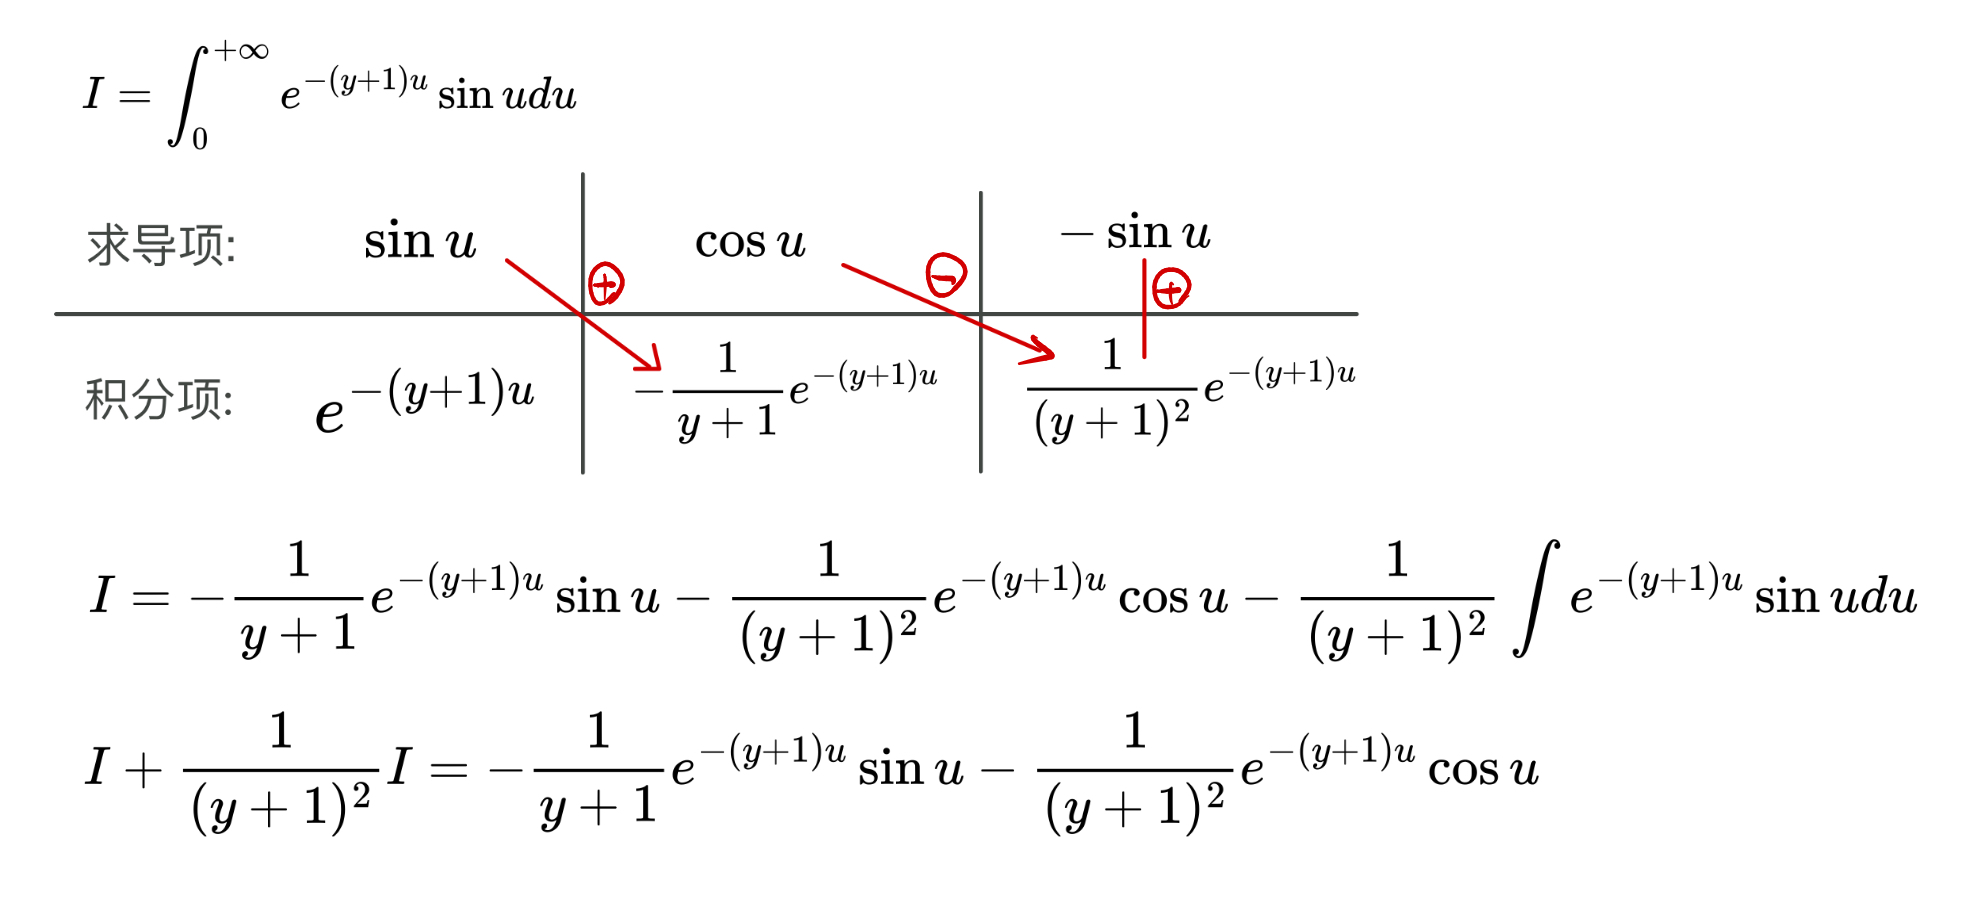
\includegraphics[width=0.9\textwidth]{表格法1.jpg} 
\end{figure}

右边将上下限代入即得
$$\int_0^1 \sin\left(\ln\frac{1}{x}\right)\frac{x^b - x^a}{\ln x}dx = \int_a^b \frac{1}{(y+1)^2 + 1} dy = \arctan(b+1) - \arctan(a+1).$$

同理可得
\begin{align*}
    \int_0^1 \cos\left(\ln\frac{1}{x}\right)\frac{x^b - x^a}{\ln x}dx &= \int_a^b dy \int_0^{+\infty} e^{-(y+1)u} \cos u \,du = \int_{a}^{b} \frac{y+1}{(y+1)^2 +1}dy \\
&= \frac{1}{2} \ln\left((y+1)^2 + 1\right) \bigg|_{y=a}^{y=b} =  \frac 1 2 \ln\frac{(b+1)^2 + 1}{(a+1)^2 + 1}. \blacksquare
\end{align*}
\end{solution}

\begin{example}
计算 $F(\alpha) = \int_{0}^{\frac{\pi}{2}} \ln\frac{1+\alpha\cos x}{1-\alpha\cos x} \cdot \frac{1}{\cos x}dx$, 其中 $\alpha \in (-1,1)$.
\end{example}

\begin{solution}
$$ F(\alpha) = \int_0^{\frac{\pi}{2}} \frac{\ln(1+\alpha\cos x) - \ln(1-\alpha\cos x)}{\cos x} dx =\int_0^{\frac{\pi}{2}} dx \int_{-\alpha}^{\alpha} \frac{1}{1+y\cos x} dy $$
此时, 令 $f(x,y) = \frac{1}{1+y\cos x}$, 该函数在区域 $[0, \frac{\pi}{2}] \times [-\alpha, \alpha]$ 上连续. 故积分次序可交换.
\begin{note}
    寻找函数的过程:
    
    积分里是$\frac{\ln(1+\alpha\cos x) - \ln(1-\alpha\cos x)}{\cos x}=\frac{\ln(1+y\cos x)}{\cos x}\bigg|_{y=-\alpha}^{y=\alpha}$,那么对$\frac{\ln(1+y\cos x)}{\cos x}$关于$y$求导即可得积分中的被积函数,在此例中求导后得到的就是$\frac{1}{1+y\cos x}$
\end{note}

\begin{align*}
\int_0^{\frac{\pi}{2}} dx \int_{-\alpha}^\alpha \frac{1}{1+y\cos x} dy &
= \int_{-\alpha}^\alpha dy \int_0^{\frac{\pi}{2}} \frac{1}{1+y\cos x} dx \\
& = \color{blue}{\boxed{\int_{-\alpha}^0 dy \int_0^{\frac{\pi}{2}} \frac{dx}{1+y\cos x} + \int_0^\alpha dy \int_0^{\frac{\pi}{2}} \frac{dx}{1+y\cos x}}} \color{red}{\text{(利用对称性)}}\\
& = \int_0^\alpha dy \int_0^{\frac{\pi}{2}} \frac{dx}{1-y\cos x} + \int_0^\alpha dy \int_0^{\frac{\pi}{2}} \frac{dx}{1+y\cos x} \\
& = \int_0^\alpha dy \int_0^{\frac{\pi}{2}} \frac{2dx}{1-y^2\cos^2 x} = \int_0^\alpha dy \int_0^{\frac{\pi}{2}} \frac{2\sec^2 x dx}{\tan^2 x + (1-y^2)} \\
& = \int_0^\alpha dy \int_0^{\frac{\pi}{2}} \frac{2}{\tan^2 x + (1-y^2)} d(\tan x) = \int_0^\alpha \frac{2}{\sqrt{1-y^2}} \arctan \frac{\tan x}{\sqrt{1-y^2}} \bigg|_0^{\frac{\pi}{2}} dy \\
& = \pi \int_0^\alpha \frac{dy}{\sqrt{1-y^2}} = \pi \arcsin \alpha, \quad \alpha \in (-1,1)
\end{align*}
$\hfill \blacksquare$
\end{solution}

\subsubsection{积分号下微分}
我们先来证明欧拉积分:
\begin{proposition}[欧拉积分]
$$I = \int_0^{\frac{\pi}{2}} \ln \cos t \, dt =I = \int_0^{\frac{\pi}{2}} \ln \sin u \, du = -\frac{\pi}{2}\ln 2$$
\end{proposition}

\begin{proof}
    考虑 $I = \int_0^{\frac{\pi}{2}} \ln \cos t \, dt$
    令 $u = \frac{\pi}{2} - t$, 则 $I = \int_0^{\frac{\pi}{2}} \ln \sin u \, du$
    将上面两式子相加有:
    $$2I = \int_0^{\frac{\pi}{2}} (\ln \cos t + \ln \sin t) \, dt = \int_0^{\frac{\pi}{2}} \ln (\frac{1}{2} \sin 2t) \, dt = -\frac{\pi}{2}\ln 2 + \int_0^{\frac{\pi}{2}} \ln (\sin 2t) \, dt$$
    令 $u = 2t$, 则积分变为 
    \begin{align*}
    \int_0^{\frac{\pi}{2}} \ln (\sin 2t) \, dt &= \frac{1}{2} \int_0^\pi \ln \sin u \, du =  \frac{1}{2} \int_0^{\frac{\pi}{2}} \ln \sin u \, du + \frac{1}{2} \int_{\frac{\pi}{2}}^{\pi} \ln \sin u \, du (\text{第二个积分中令}v = \frac{\pi}{2}- u)\\
     &=  \frac{1}{2} \int_0^{\frac{\pi}{2}} \ln \sin u \, du + \frac{1}{2} \int_{0}^{\frac{\pi}{2}} \ln \cos v \, dv =\frac{1}{2} \cdot 2I = I
    \end{align*}
    那么 $2I = -\frac{\pi}{2}\ln 2 + I \Rightarrow I = -\frac{\pi}{2}\ln 2$ $\hfill \blacksquare$
\end{proof}


\begin{example}[$\bigstar$]{\label{ex:integral-parameter_1}}
    计算$F(\theta)= \int_{0}^{\pi} \ln (1+\theta \cos x) \mathrm{d} x$,其中$\theta \in [-1,1]$.
\end{example}

\begin{solution}
令$f(x, \theta) = \ln(1+\theta \cos x)$, 其中$\theta \in [-1, 1]$. 注意到当$\theta = \pm 1$时, $f(x, \theta)$可能无界. 先对这两种情形讨论.
$1^\circ \theta = \pm 1$时
$$F(1) = \int_{0}^{\pi} \ln(1+\cos x)dx = \int_{0}^{\pi} \ln(2\cos^2\frac{x}{2})dx = \pi\ln2 + 2\int_{0}^{\pi}\ln(\cos\frac{x}{2})dx$$$$= \pi\ln2 + 4\int_{0}^{\pi}\ln(\cos\frac{x}{2})d(\frac{x}{2}) = \pi\ln2 + 4\int_{0}^{\frac{\pi}{2}}\ln\cos x dx = \pi\ln2 - 4 \times \frac{\pi}{2}\ln2$$$$= -\pi\ln2$$
同理$F(-1) = \int_{0}^{\pi} \ln(1-\cos x)dx = \pi\ln2 + 4\int_{0}^{\frac{\pi}{2}}\ln\sin x dx = -\pi\ln2$

$2^\circ$ 当$\theta \in (-1, 1)$时
$f'_{\theta}(x, \theta) = \frac{\cos x}{1+\theta \cos x}$, 那么此时$f(x, \theta), f'_{\theta}(x, \theta)$在$[0, \pi] \times (-1, 1)$均连续, 那么$F(\theta)$在$(-1, 1)$可导.
又因为
\begin{equation*}
F(-\theta) = \int_{0}^{\pi} \ln(1-\theta\cos x)dx \xlongequal{t=\pi-x} \int_{0}^{\pi} \ln(1+\theta\cos t)dt = F(\theta)
\end{equation*}

从而$F(\theta)$为偶函数, 那样就先求它在$(x, \theta) \in [0, \pi] \times [0, 1)$上的情形.
考虑
\begin{align*}
    F'(\theta) &= \int_{0}^{\pi} \frac{\cos x}{1+\theta \cos x}dx = \color{blue}{\frac{1}{\theta}\int_{0}^{\pi}\frac{1+\theta\cos x - 1}{1+\theta\cos x}dx} = \frac{1}{\theta}\int_{0}^{\pi}(1-\frac{1}{1+\theta\cos x})dx \\
               &= \frac{\pi}{\theta} - \frac{1}{\theta}\int_{0}^{\pi}\frac{1}{1+\theta\cos x}dx = \frac{\pi}{\theta} - \frac{\pi}{\theta\sqrt{1-\theta^2}}, |\theta|<1
\end{align*}


那么
\begin{align*}
    F(\theta)&=\int(\frac{\pi}{\theta}-\frac{\pi}{\theta\sqrt{1-\theta^2}})d\theta = \pi\ln\theta - \pi\int\frac{1}{\theta\sqrt{1-\theta^2}}d\theta+C =\pi \ln \theta - \color{blue}{\int\frac{\theta^{-2}\pi}{\sqrt{\theta^{-2}-1}}\mathrm{d} \theta +C}\\
             &=\pi \ln \theta + \int\frac{\pi}{\sqrt{\theta^{-2}-1}}\mathrm{d} \theta^{-1} +C = \pi \ln \theta +\pi \ln(\theta^{-1}+\sqrt{\theta^{-2}-1})+C=\pi \ln (1+ \sqrt{1-\theta^2}) +C
\end{align*}

当$\theta=0, F(0)=\lim\limits_{\theta \to 0} F(\theta) = \pi\ln2+C$, 而$F(0)=0$, 故$C=-\pi\ln2$.
那么$F(\theta)=\pi\ln\frac{1+\sqrt{1-\theta^2}}{2}$, 此时$F(\theta)$为偶函数.
那么在$(-1, 1)$上,$F(\theta)=\pi\ln\frac{1+\sqrt{1-\theta^2}}{2}$.

综上由$1^\circ, 2^\circ$得$F(\theta)=\pi\ln\frac{1+\sqrt{1-\theta^2}}{2}, \theta \in [-1, 1]$.
$\hfill \blacksquare$
\end{solution}

\begin{note}
    与本题类似的还有
        先计算含参变量积分$$I(\alpha) = \int _0^{\pi} \ln(\alpha +\cos x)dx,\alpha > 1$$
    易知$f(\alpha,x)$可导,且
    $$ I'(\alpha) = \int_{0}^{\pi} \frac{1}{\alpha + \cos x} dx \stackrel{t=\tan\frac{x}{2}}{=} \int_{0}^{+\infty} \frac{1}{\alpha + \frac{1-t^2}{1+t^2}} \cdot \frac{2 dt}{1+t^2}  = 2 \int_{0}^{+\infty} \frac{dt}{\alpha(1+t^2) + 1-t^2} = 2 \int_{0}^{+\infty} \frac{dt}{\alpha+1 + (\alpha-1)t^2} $$
    $$ = \frac{2}{\sqrt{\alpha^2-1}} \int_{0}^{+\infty} \frac{1}{1 + \left(\sqrt{\frac{\alpha-1}{\alpha+1}}t\right)^2} d\left(\sqrt{\frac{\alpha-1}{\alpha+1}}t\right)  = \frac{2}{\sqrt{\alpha^2-1}} \left( \arctan \sqrt{\frac{\alpha-1}{\alpha+1}}t \right) \Bigg|_{0}^{+\infty} = \frac{2}{\sqrt{\alpha^2-1}} \cdot \frac{\pi}{2} = \frac{\pi}{\sqrt{\alpha^2-1}} $$
    那么$I(\alpha) = \pi ln(\alpha +\sqrt{\alpha^2 -1})+C$,且$I(1)=\pi ln(1+0)+C=C$.

    而$I(1) = -\pi\ln 2$(降次加欧拉积分即可得).那么$C = I(1) = -\pi \ln 2$,则
    $$I(\alpha) = \pi ln(\alpha +\sqrt{\alpha^2 -1})+C= \pi ln(\alpha +\sqrt{\alpha^2 -1})-\pi \ln 2=\pi \ln \frac{\alpha+\sqrt{\alpha^2 -1}}{2}  $$$\hfill \blacksquare$
\end{note}

\begin{example}[$\bigstar$]
    计算$F(a) = \int_0^{\pi} \ln(a^2 -2a \cos x +1) \mathrm{d} x$.
\end{example}

\begin{solution}[解法1]


\begin{remark}
考虑$a^2-2a\cos x+1$, 视为$a$的二次函数.
有$\Delta=4\cos^2x-4 \le 0$. 则$\Delta < 0$时, $f(x,a)=\ln(a^2-2a\cos x+1)$有意义.
当$\Delta=0$, 即$\cos^2x=1$, 即$\cos x=\pm 1$时, $f(x,a)=\ln(a\mp 1)^2$可能无意义.
此时需对$a=\pm 1$进行讨论.
\end{remark}

$1^\circ$ 当$a=\pm 1$时
$F(1) = \int_{0}^{\pi}\ln(1-2\cos x+1)dx = \int_{0}^{\pi}(\ln 2+\ln(1-\cos x))dx = \pi\ln2 - \pi\ln2=0$,
同理有$F(-1) = \int_{0}^{\pi}\ln(1+2\cos x+1)dx=0$

$2^\circ$ 当$|a|<1$时. $F(-a)=F(a)$. 故先考虑$0<a<1$.
$f_a(x,a) = \frac{2a-2\cos x}{a^2-2a\cos x+1}$,由于$f(x,a)$,$f_a(x,a)$在$[0,\pi] \times (0,1)$上连续, 故可以求导.
即有$F'(a)=\int_{0}^{\pi}\frac{2a-2\cos x}{a^2-2a\cos x+1}dx$

\begin{align*}
    F'(a) &= \color{blue}{\frac{1}{a}\int_{0}^{\pi}\frac{a^2-2a\cos x+1-(1-a^2)}{a^2-2a\cos x+1}dx = \frac{1}{a}\int_{0}^{\pi}(1-\frac{1-a^2}{a^2-2a\cos x+1})dx}\\
          &= \frac{\pi}{a} - \frac{1-a^2}{a}\int_{0}^{\pi}\frac{1}{a^2+1-2a\cos x}dx = \frac{\pi}{a} - \frac{1-a^2}{a(1+a^2)}\int_{0}^{\pi}\frac{1}{1-\frac{2a}{1+a^2}\cos x}dx \\
          &= \frac{\pi}{a} - \frac{1-a^2}{a(1+a^2)}\frac{\pi}{\sqrt{1-(\frac{2a}{1+a^2})^2}} = \frac{\pi}{a} - \frac{1-a^2}{a(1+a^2)}\frac{\pi(a^2+1)}{|a^2-1|} = \frac{\pi}{a} - \frac{\pi}{a}\cdot\frac{1-a^2}{1-a^2} = 0
\end{align*}

从而$F(a)=C$. 又由$F(0)=0$, 而$\lim\limits_{a\to 0}F(a)=0$, 故$C=0$, 那么$F(a)=0$.
且$F(a)$为偶函数, 那么当$-1<a<1$时, $F(a)=0$.

$3^\circ$ 当$|a|>1$时, $|\frac{1}{a}|<1$,那么有

\begin{align*}
F(\frac{1}{a}) &= \int_{0}^{\pi}\ln\left(\frac{1}{a^2}-\frac{2\cos x}{a}+1\right)dx = \int_{0}^{\pi}\ln\frac{1-2a\cos x+a^2}{a^2}dx \\
&= \int_{0}^{\pi}\ln(1-2a\cos x+a^2)dx - 2\pi\ln|a| = F(a)-2\pi\ln|a|
\end{align*}

又由于$F(\frac{1}{a}) = 0 $,故 $F(a) = \begin{cases} 2\pi\ln|a|, & |a| \geq  1 \\ 0, & |a|<  1 \end{cases}$
$\hfill \blacksquare$
\end{solution}

\begin{solution}[解法2]
\begin{align*}
F(a) &= \int_{0}^{\pi} \ln(a^2 - 2a\cos x + 1)dx = \int_{0}^{\pi} \ln(a^2+1-2a\cos x)dx \\
&= \int_{0}^{\pi} \ln\left((a^2+1)\left(1-\frac{2a}{a^2+1}\cos x\right)\right)dx = \int_{0}^{\pi}\ln(a^2+1)dx + \int_{0}^{\pi}\ln\left(1-\frac{2a}{a^2+1}\cos x\right)dx \\
&= \pi\ln(a^2+1) + \int_{0}^{\pi}\ln\left(1-\frac{2a}{a^2+1}\cos x\right)dx, \quad \text{由于 } |\frac{2a}{a^2+1}| \le 1, \text{再利用上题结论} \\
&= \pi\ln(a^2+1) + \pi\ln\frac{1+\sqrt{1-\left(\frac{2a}{a^2+1}\right)^2}}{2} = \pi\ln\frac{a^2+1}{2} + \pi\ln\left(1+\sqrt{1-\frac{4a^2}{(a^2+1)^2}}\right) \\
&= \pi\ln\frac{a^2+1}{2} + \pi\ln\left(1+\sqrt{\frac{a^4+2a^2+1-4a^2}{(a^2+1)^2}}\right) = \pi\ln\frac{a^2+1}{2} + \pi\ln\left(1+\sqrt{\frac{(a^2-1)^2}{(a^2+1)^2}}\right) \\
&= \pi\ln\frac{a^2+1}{2} + \pi\ln\left(1+\frac{|a^2-1|}{a^2+1}\right) = \pi\ln\frac{a^2+1+|a^2-1|}{2} \\
&= \begin{cases}
2\pi\ln|a|, & |a| \ge 1 \\
0, & |a| < 1
\end{cases}
\end{align*}
$\hfill \blacksquare$
\end{solution}

\begin{solution}[解法3]
        当 $|a| < 1$ 时,注意到$I(a)=I(-a)$,则有:
    \begin{align*} 2I(a) &= \int_{0}^{\pi} \ln(1-2a\cos x + a^2)dx + \int_{0}^{\pi} \ln(1+2a\cos x + a^2)dx \\ &= \int_{0}^{\pi} \ln(1-2a^2\cos 2x + a^4)dx = \frac{1}{2} \int_{0}^{2\pi} \ln(1-2a^2\cos x + a^4)dx \\ &= \int_{0}^{\pi} \ln(1-2a^2\cos x + a^4)dx = I(a^2)\end{align*}
    从而:
    $$ I(a) = \lim\limits_{n \to \infty} \frac{I(a^{2^n})}{2^n} $$
    考虑极限
    $$ \lim\limits_{n \to \infty} I(a^{2^n}) = \lim\limits_{n \to \infty} \int_{0}^{\pi} \ln(1-2a^{2^n}\cos x + a^{2n+1})dx = \int_{0}^{\pi} \ln 1 dx = 0 $$
    因此 $I(a)=0$。

    当 $|a|=1$ 时可以直接计算出积分为0.
    当 $|a| > 1$ 时:
    $$ I(a) = \int_{0}^{\pi} \ln a^2 dx + \int_{0}^{\pi} \ln(1-2\frac{1}{a}\cos x + \frac{1}{a^2})dx = 2\pi \ln |a| $$
综上可得
\begin{align*}
 I(a)= \begin{cases}
    2\pi\ln|a|, & |a| \ge 1 \\
    0, & |a| < 1
\end{cases}
\end{align*}
$\hfill \blacksquare$
\end{solution}

\begin{example}
计算 $I = \int_{0}^{\frac{\pi}{2}} \ln(a^2\sin^2x+b^2\cos^2x)\mathrm{d} x$, 其中 $a^2+b^2 > 0$.
\end{example}

\begin{solution}[解法1(利用例题\ref{ex:integral-parameter_1})]
\begin{align*}
I &= \int_{0}^{\frac{\pi}{2}} \ln(a^2(1-\cos^2x)+b^2\cos^2x)dx = \int_{0}^{\frac{\pi}{2}} \ln(a^2+(b^2-a^2)\cos^2x)dx \\
&= \int_{0}^{\frac{\pi}{2}} \ln\left[a^2+(b^2-a^2)\frac{1+\cos 2x}{2}\right]dx = \int_{0}^{\frac{\pi}{2}} \ln\left[\frac{a^2+b^2}{2}+\frac{b^2-a^2}{2}\cos 2x\right]dx \\
&= \int_{0}^{\frac{\pi}{2}} \ln\left[\frac{a^2+b^2}{2}\left(1+\frac{b^2-a^2}{a^2+b^2}\cos 2x\right)\right]dx + \frac{\pi}{2}\ln 2 \\
&\xlongequal{t=2x} \frac{1}{2}\int_{0}^{\pi}\ln\left(1+\frac{b^2-a^2}{a^2+b^2}\cos t\right)dt + \frac{\pi}{2}\ln\frac{a^2+b^2}{2} = \frac{\pi}{2}\ln\frac{1+\sqrt{1-\left(\frac{b^2-a^2}{a^2+b^2}\right)^2}}{2} + \frac{\pi}{2}\ln\frac{a^2+b^2}{2} \\
&= \frac{\pi}{2}\ln\frac{(a^2+b^2)+\sqrt{(a^2+b^2)^2-(b^2-a^2)^2}}{4} = \frac{\pi}{2}\ln\frac{a^2+b^2+2|ab|}{4} \quad = \pi\ln\frac{|a|+|b|}{2} \blacksquare
\end{align*}
\end{solution}

\begin{solution}[解二]
首先设$a, b>0$固定值, 记$f(t) = \int_{0}^{\frac{\pi}{2}} \ln(a^2\sin^2x+t^2\cos^2x)dx$
且$F(x,t) = \ln(a^2\sin^2x+t^2\cos^2x)$
$F_t(x,t) = \frac{2t\cos^2x}{a^2\sin^2x+t^2\cos^2x}$, 显然$F(x,t)$及$F_t(x,t)$在 \fcolorbox{black}{yellow}{$[0, \frac{\pi}{2}] \times [a,b]$或$([0, \frac{\pi}{2}] \times [b,a])$上连续.}
\begin{align*}
\text{从而 } f'(t) &= \int_{0}^{\frac{\pi}{2}}\frac{2t\cos^2x}{a^2\sin^2x+t^2\cos^2x}dx = \int_{0}^{\frac{\pi}{2}}\frac{2t}{a^2\tan^2x+t^2}dx \\
&\xlongequal{u=\tan x} \int_{0}^{+\infty} \frac{2t}{a^2u^2+t^2}\cdot\frac{1}{u^2+1}du \\
&\color{blue}{= \int_{0}^{+\infty} 2t\cdot \frac{1}{a^2-t^2}\left(\frac{a^2}{a^2u^2+t^2}-\frac{1}{u^2+1}\right)du }\\
&= \frac{2t}{a^2-t^2}\left[\frac{a}{t}\arctan\frac{au}{t} - \arctan u\right]_0^{+\infty} \\
&= \frac{2t}{a^2-t^2}\left(\frac{a}{t}\cdot\frac{\pi}{2}-\frac{\pi}{2}\right) = \frac{2t}{a^2-t^2}\frac{\pi(a-t)}{2t} = \frac{\pi}{a+t}
\end{align*}
那么$f(t) = \pi\ln(a+t)+C$. 由于$f(a) = \int_{0}^{\frac{\pi}{2}}\ln(a^2)dx = \pi\ln a$
那么$f(a) = \pi\ln(2a)+C = \pi\ln a$, 那么$C = -\pi\ln 2$. 故$f(t) = \pi\ln\frac{a+t}{2}$.
$f(b) = \pi\ln\frac{a+b}{2}$, 即$I = \pi\ln\frac{a+b}{2}$, $a>0, b>0$.

由于I关于$a,b$均为偶函数, ($a\ne 0, b\ne 0$时), 故$I=\pi\ln\frac{|a|+|b|}{2}$.
当$a=0, b\ne 0$时, $I = \int_{0}^{\frac{\pi}{2}}\ln(b^2\cos^2x)dx = \int_{0}^{\frac{\pi}{2}}2\ln\cos x dx + \pi\ln|b| = -\frac{\pi}{2}\ln 2 \times 2 + \pi\ln|b| = \pi\ln\frac{|b|}{2}$.
同理$a\ne 0, b=0$时, $I=\pi\ln\frac{|a|}{2}$.
故总可知$a^2+b^2>0$时, 有$I=\pi\ln\frac{|a|+|b|}{2}$.
$\hfill \blacksquare$
\end{solution}

\begin{example}
    计算$F(a)= \int_{0}^{\frac{\pi}{2}} \frac{\arctan(a\tan x)}{\tan x } \mathrm d x$.
\end{example}
\begin{solution}
解: 注意到$F(a)$是奇函数, 故只需讨论$a >  0$的情况:
设 $f(x,a) = \frac{\arctan(a\tan x)}{\tan x}$, $f_a(x,a) = \frac{1}{\tan x}\cdot\frac{1}{1+a^2\tan^2x}\cdot\tan x = \frac{1}{1+a^2\tan^2x}$.
显然$f(x,a)$和$f_a(x,a)$在$[0, \frac{\pi}{2}] \times (0, +\infty)$上连续. 故$F(a)$在$(0, +\infty)$上可导, 那么
\begin{align*}
F'(a) &= \int_{0}^{\frac{\pi}{2}} \frac{1}{1+a^2\tan^2x}dx \xlongequal{u=\tan x} \int_{0}^{+\infty}\frac{1}{1+a^2u^2}\cdot\frac{1}{1+u^2}du \\
&\color{blue}{= \frac{1}{a^2-1}\int_{0}^{+\infty}\left(\frac{a^2}{1+a^2u^2}-\frac{1}{1+u^2}\right)du} \\
&= \frac{1}{a^2-1}\left[a\cdot\arctan(au) - \arctan u\right]_0^{+\infty} \\
&= \frac{1}{a^2-1}\left(\frac{\pi}{2}a-\frac{\pi}{2}\right) = \frac{\pi}{2(a+1)}
\end{align*}
那么$F(a)=\frac{\pi}{2}\ln(a+1)+C$. 由于$F(0)=0$, 那么$0=\lim\limits_{a\to 0^+}F(a)=C$.
从而$F(a)=\frac{\pi}{2}\ln(a+1), a>0$.
由于$F(a)$为奇函数, 那么$a<0$, 则$-a>0$.
从而$F(a)=-F(-a)=-\frac{\pi}{2}\ln(-a+1)$.


综上$F(a) = \begin{cases} \frac{\pi}{2}\ln(a+1), & a\ge 0 \\ -\frac{\pi}{2}\ln(1-a), & a<0 \end{cases}$ $\hfill \blacksquare$
\end{solution}


\begin{example}
    计算$I = \int_{0}^{1} \frac{\ln (1+x)}{1+x^2}$.
\end{example}
\begin{remark}
    本题令$f(x,\alpha) = \frac{\ln(1+\alpha x)}{1+x^2}$,记$F(\alpha) = \int_{0}^{1} f(x,\alpha) \mathrm d x$,那么同样可以使用含参变量积分(区间取$[0,1] \times [0,1]$),但针对本题过于繁琐,本题换元加区间再现即可.
\end{remark}

\begin{solution}
设$x=\tan t$, 那么$t=\arctan x$
\begin{align*}
I &= \int_{0}^{\frac{\pi}{4}}\frac{\ln(1+\tan t)}{1+\tan^2 t}\cdot\frac{1}{\cos^2 t}dt = \int_{0}^{\frac{\pi}{4}}\ln(1+\tan t)dt \\
&= \int_{0}^{\frac{\pi}{4}}\ln\frac{\cos t+\sin t}{\cos t}dt = \int_{0}^{\frac{\pi}{4}}\ln\frac{\sqrt{2}\sin(t+\frac{\pi}{4})}{\cos t}dt \\
&= \int_{0}^{\frac{\pi}{4}}\ln(\sqrt{2}\sin(t+\frac{\pi}{4}))dt - \int_{0}^{\frac{\pi}{4}}\ln\cos t dt \\
&= \frac{\pi}{8}\ln 2 + \int_{0}^{\frac{\pi}{4}}\ln\sin(t+\frac{\pi}{4})dt - \int_{0}^{\frac{\pi}{4}}\ln\cos t dt
\end{align*}

对于



\begin{align*}
    \int_{0}^{\frac{\pi}{4}}\ln\cos t dt &\xlongequal[u=\frac{\pi}{4}-t]{t=\frac{\pi}{4}-u} \boxed{-\int_{\frac{\pi}{4}}^{0}\ln\cos(\frac{\pi}{4}-u)du = \int_{0}^{\frac{\pi}{4}}\ln\sin[\frac{\pi}{2}-(\frac{\pi}{4}-u)]du}\\
&= \int_{0}^{\frac{\pi}{4}}\ln\sin(u+\frac{\pi}{4})du = \int_{0}^{\frac{\pi}{4}}\ln\sin(t+\frac{\pi}{4})dt
\end{align*}

从而$I=\frac{\pi}{8}\ln 2 \quad  $ $\hfill \blacksquare$
\end{solution}


\begin{example}
设
$$f(x) = \int_{0}^{1} \frac{e^{-x^2(y^2+1)}}{y^2+1} dy, g(x) = \left(\int_{0}^{x} e^{-y^2} dy\right)^2$$
解答下面两个问题:
(1) 证明:$x \ge 0$ 时,$f(x) + g(x) = \frac{\pi}{4}$.
(2) 证明欧拉-泊松积分:$\int_{0}^{+\infty} e^{-x^2} dx = \frac{\sqrt{\pi}}{2}$.
\end{example}

\begin{solution}
(1) 当 $x \ge 0$ 时, 可知
$$f'(x) = -2x \int_{0}^{1} e^{-x^2(y^2+1)} dy = -2xe^{-x^2} \int_{0}^{1} e^{-x^2y^2} dy,$$
$$g'(x) = 2e^{-x^2} \int_{0}^{x} e^{-y^2} dy \xlongequal{\boxed{y=xt}} 2xe^{-x^2} \int_{0}^{1} e^{-x^2t^2} dt.$$
所以 $f'(x) + g'(x) = 0$, 进而 $f(x)+g(x) = f(0)+g(0) = \int_{0}^{1} \frac{dy}{y^2+1} = \frac{\pi}{4}$.
(2) 注意到当 $y \in [0, 1]$ 时,有
$$0 < \frac{e^{-x^2(y^2+1)}}{y^2+1} \le e^{-x^2(y^2+1)} \le e^{-x^2} \to 0~(x \to +\infty).$$
所以当 $x \to +\infty$ 时,$\frac{e^{-x^2(y^2+1)}}{y^2+1}$ 关于 $y \in [0, 1]$ 一致收敛于零,从而
$$\lim\limits_{x \to +\infty} f(x) = \lim\limits_{x \to +\infty} \int_{0}^{1} \frac{e^{-x^2(y^2+1)}}{y^2+1} dy = \int_{0}^{1} \lim\limits_{x \to +\infty} \frac{e^{-x^2(y^2+1)}}{y^2+1} dy = \int_{0}^{1} 0 dy = 0.$$
从而根据 (1) 可知
$$\left(\int_{0}^{+\infty} e^{-y^2} dy\right)^2 = \lim\limits_{x \to +\infty} g(x) = \lim\limits_{x \to +\infty} \left(\frac{\pi}{4} - f(x)\right) = \frac{\pi}{4},$$
即有 
\fcolorbox{black}{yellow}{$\int_{0}^{+\infty} e^{-x^2} dx = \frac{\sqrt{\pi}}{2}$}.
$\hfill \blacksquare$
\end{solution}

\begin{example}
设 $f(x, y)$ 在 $\mathbb{R}^2$ 上存在二阶连续偏导数, $f_{xx} + f_{yy} = 0$, 且对固定的 $y$, $f_x(x, y)$ 与 $f_y(x, y)$ 是关于 $x$ 的以 $2\pi$ 为周期的函数, 证明 $\int_{0}^{2\pi} (f_x^2 - f_y^2) dx$ 为常值.
\end{example}

\begin{solution}
记 $g(y) = \int_{0}^{2\pi} (f_x^2 - f_y^2) dx$,由于$f(x,y)$在$\mathbb R^2$上存在二阶连续偏导,故$f_x,f_y,f_{xx},f_{yy},f_{xy}$均连续。从而$g(x,y)$可导,
 则根据已知有
\begin{align*}
g'(y) &= \int_{0}^{2\pi} (2f_x f_{xy} - 2f_y f_{yy}) dx = 2 \int_{0}^{2\pi} f_x f_{xy} dx - 2 \int_{0}^{2\pi} f_y f_{yy} dx \\
&= \boxed{2 \int_{0}^{2\pi} f_x d(f_y)} - 2 \int_{0}^{2\pi} f_y f_{yy} dx = \boxed{2f_x f_y \Big|_{0}^{2\pi}} - 2 \int_{0}^{2\pi} f_y f_{xx} dx - 2 \int_{0}^{2\pi} f_y f_{yy} dx \\
&= 0 - 2 \int_{0}^{2\pi} f_y f_{xx} dx - 2 \int_{0}^{2\pi} f_y f_{yy} dx = 0.
\end{align*}
这说明 $g(y) = \int_{0}^{2\pi} (f_x^2 - f_y^2) dx$ 为常值.
$\hfill \blacksquare$
\end{solution}

\begin{example}
证明 $\int_{0}^{2\pi} e^{t \cos\theta} \cos(t \sin\theta) d\theta = 2\pi$.
\end{example}

\begin{solution}
记 $F(t) = \int_{0}^{2\pi} e^{t \cos\theta} \cos(t \sin\theta) d\theta$, 则 $F(0) = 2\pi$.  可知
$$F'(t) = \int_{0}^{2\pi} [e^{t \cos\theta} \cos\theta \cos(t \sin\theta) - e^{t \cos\theta} \sin\theta \sin(t \sin\theta)] d\theta = \int_{0}^{2\pi} e^{t \cos\theta} \cos(t \sin\theta + \theta) d\theta.$$
我们发现此时$F'(t)$不一定为0,故不能通过前面的一样套路.注意到 $F^{(n)}(t) = \int_{0}^{2\pi} e^{t \cos\theta} \cos(t \sin\theta + n\theta) d\theta$, 且有$$F^{(n)}(0) = 0, \quad n=1, 2, 3, \cdots$$
我们考虑Lagrange余项的Taylor展开, 对每个正整数 $n$, 存在介于 0 与 $t$ 之间的 $\xi$, 使得
\begin{equation*}
\boxed{F(t) = F(0) + \cdots + 0 + \frac{t^n}{n!}F^{(n)}(\xi) = 2\pi + \frac{t^n}{n!}F^{(n)}(\xi). }
\end{equation*}
注意到
$$|F^{(n)}(\xi)| = \left| \int_{0}^{2\pi} e^{\xi \cos\theta} \cos(\xi \sin\theta + n\theta) d\theta \right| \le \int_{0}^{2\pi} e^{|t|} d\theta = 2\pi e^{|t|},$$
所以对固定的 $t \in (-\infty, +\infty)$, 有 $\lim\limits_{n \to \infty} \frac{t^n}{n!} F^{(n)}(\xi) = 0$, 从而关于 $n \to \infty$ 取极限可得 $F(t) = 2\pi$.
$\hfill \blacksquare$
\end{solution}

\section{含参变量反常积分}

\subsection{基本定理以及简单应用}
\begin{definition}[含参量反常积分]
设 $f(x,t)$ 在 $\{(x,t) | x \in [c, +\infty), t \in I\}$ 上有定义, 其中 $I$ 为一个区间, 若对每个固定的 $t \in I$, 反常积分
\begin{equation}{\label{eq13.6}}
\int_{c}^{+\infty} f(x,t) dx 
\end{equation}
都收敛, 则它的值是 $t$ 在 $I$ 上取值的函数, 记为
\begin{equation}{\label{eq13.7}}
\varphi(t) = \int_{c}^{+\infty} f(x,t) dx, \quad t \in I.   
\end{equation}
称 $\varphi(t)$ 为定义在区间 $I$ 上的含参量 $t$ 的无穷限反常积分, 简称含参量反常积分.
\end{definition}

\begin{remark}
    同样可定义含参量的瑕积分,通过倒数变换可以转化为含参量的无穷积分.

    \fcolorbox{blue}{yellow}{函数项级数 =数项级数 +“一致”,对应有:含参反常积分 = 反常积分 +"一致”.}
    
    那么本节的核心任务是研究带有参数的反常积分关于参量的\underline{一致收敛性},另外,函数项级数可看成离散求和的含参量反常积分,其中函数的自变最对应着参变量,即$\sum u_n(x)$中的$x$对应$\int_{c}^{\infty}f(x,t)\mathrm d x$中的参变量$t$,因此含参量反常积分的很多方法和结论都与函数项级数极为相似
\end{remark}

\begin{definition}[含参量反常积分的一致收敛]
对于含参量积分 (\ref{eq13.6}) 与函数 (\ref{eq13.7}), 若对任意的 $\epsilon > 0$, 总存在 $N > 0$, 使得 $M > N$ 时, \textcolor{blue}{对任意的 $t \in I$(即$N$与$t$无关)}, 有
$$ \left| \int_{c}^{M} f(x,t) dx - \varphi(t) \right| = \left| \int_{M}^{+\infty} f(x,t) dx \right| < \epsilon, $$
则称含参量反常积分 (\ref{eq13.6}) 在区间 $I$ 上\textcolor{blue}{一致收敛}于 $\varphi(t)$, 或简称为 $\varphi(t)$ 在 $I$ 上一致收敛. 若 $\varphi(t)$ 在 $I$ 内的任意闭区间上一致收敛, 则称 $\varphi(t)$ 在 $I$ 上\textbf{内闭一致收敛}.
\end{definition}

\begin{remark}
若 $\int_{c}^{+\infty} f(x,t) dx$ 在 $I$ 上收敛, 那么 $\int_{c'}^{+\infty} f(x,t) dx$ 在 $I$ 上一致收敛等价于 $\int_{c}^{+\infty} f(x,t) dx$ 在 $I$ 上一致收敛, 其中 $c' \ge c$ 为任意常数.
\end{remark}
\begin{theorem}[柯西准则]
含参量积分 (\ref{eq13.6}) 在区间 $I$ 上一致收敛的充要条件为: 对任意的 $\varepsilon > 0$, 存在 $M > c$, 使得当 $A_1, A_2 > M$ 时, 对任意的 $t \in I$, 都有
$$ \left| \int_{A_1}^{A_2} f(x,t) dx \right| < \varepsilon. $$
\end{theorem}

\begin{theorem}{\label{反常积分一致收敛的确界法}}
含参量积分 (\ref{eq13.6}) 在区间 $I$ 上一致收敛的充要条件为
$$ \lim\limits_{M \to +\infty} \sup_{t \in I} \left| \int_{M}^{+\infty} f(x,t) dx \right| = 0. $$
\end{theorem}

\begin{theorem}[魏尔斯特拉斯判别法(M判别法)]
若存在函数 $g(x)$ 满足
$$ |f(x,t)| \le g(x), \quad x \in [c, +\infty), t \in I, $$
且 $\int_{c}^{+\infty} g(x) dx$ 收敛, 则含参量积分 (\ref{eq13.6}) 在 $I$ 上一致收敛.
\end{theorem}
\begin{remark}
    证明可用柯西收敛准则,$|\int_{A_1}^{A_2} f(x,t) dx| \le \int_{A_1}^{A_2} g(x) dx < \varepsilon$, 其中 $g(x)$ 满足 $\int_{c}^{+\infty} g(x) dx$ 收敛.
\end{remark}

\begin{proof}
$\forall \varepsilon > 0$, $\exists M > c$, 当 $A_1, A_2 > M$ 时 $\forall t \in I$, 由于 $\int_c^{+\infty} g(x)dx$ 收敛, 则有
$$\left| \int_{A_1}^{A_2} f(x,t) dx \right| \le \int_{A_1}^{A_2} |f(x,t)| dx \le \int_{A_1}^{A_2} g(x) dx < \varepsilon$$
那么由Cauchy收敛准则知 $\int_c^{+\infty} f(x,t) dx$ 在 $I$ 上一致收敛.
$\hfill \blacksquare$
\end{proof}

\begin{example}
设 $f(x,t)$ 在 $[c, +\infty) \times I$ 上连续, 且成立不等式 $|f(x,t)| \le F(x,t)$. 若 $\int_{c}^{+\infty} F(x,t) dx$ 在 $I$ 上一致收敛, 证明 $\int_{c}^{+\infty} f(x,t) dx$ 在 $I$ 上绝对一致收敛.
\end{example}

\begin{proof}
证:$\forall \varepsilon > 0, \exists M > c,$ 当 $A_1, A_2 > M$ 时, $\forall t \in I,$ 有 $|\int_{A_1}^{A_2} f(x,t)dx| < \varepsilon$
那么
$$ \left| \int_{A_1}^{A_2} f(x,t)dx \right| \le \int_{A_1}^{A_2} |F(x,t)|dx < \varepsilon $$
那么由 Cauchy 收敛准则知 $\int_c^{+\infty} f(x,t) dx$ 在 $I$ 上绝对一致收敛.
$\hfill \blacksquare$
\end{proof}

\begin{example}{\label{ex13.2.2}}
讨论 $\varphi(x) = \int_{0}^{+\infty} xe^{-xy} dy$ 在 $(0, +\infty)$ 上的一致收敛性.
\end{example}

\begin{proof}
$$ \lim\limits_{M \to +\infty} \sup_{x \in (0, +\infty)} \left| \int_M^{+\infty} xe^{-xy} dy \right| = \lim\limits_{M \to +\infty} \sup_{x \in (0, +\infty)}  \left| -e^{-xy} |_{y=M}^{y=+\infty} \right|  = \lim\limits_{M \to +\infty} \sup_{x \in (0, +\infty)} e^{-xM} = 1 \neq 0 $$
从而 $\varphi(x)$ 在 $(0, +\infty)$ 上不一致收敛.

但考虑 $\forall x_0 > 0$, $x$ 在 $[x_0, +\infty)$ 区间上时
$$ \lim\limits_{M \to +\infty} \sup_{x \in [x_0, +\infty)} \left| \int_M^{+\infty} x e^{-xy} dy \right| = \lim\limits_{M \to +\infty} \sup_{x \in [x_0, +\infty)} e^{-xM} = \lim\limits_{M \to +\infty} e^{-x_0 M} = 0 $$
从而 $\varphi(x)$ 在 $[x_0, +\infty)$ 上一致收敛, $\forall x_0 > 0$.
$\hfill \blacksquare$
\end{proof}

\begin{example}{\label{ex13.2.3}}
讨论 $\varphi(u) = \int_{0}^{+\infty} \sqrt{u}e^{-ux^2} dx$ 在 $u \in (0, +\infty)$ 上的一致收敛性.
\end{example}

\begin{proof}
1°
$$ \lim\limits_{M \to +\infty} \sup_{u \in (0, +\infty)} \left| \int_M^{+\infty} \sqrt{u} e^{-ux^2} dx \right| = \lim\limits_{M \to +\infty} \sup_{u \in (0, +\infty)} \left| \int_M^{+\infty} e^{-(\sqrt{u}x)^2} d(\sqrt{u}x) \right| $$
令 $t = \sqrt{u}x$
$$ \lim\limits_{M \to +\infty} \sup_{u \in (0, +\infty)} \left| \int_{\sqrt{u}M}^{+\infty} e^{-t^2} dt \right| = \lim\limits_{M \to +\infty} \sup_{u \in (0, +\infty)} \int_{\sqrt{u}M}^{+\infty} e^{-t^2} dt = \int_0^{+\infty} e^{-t^2} dt = \frac{\sqrt{\pi}}{2} \neq 0 $$
从而 $\varphi(u)$ 在 $u \in (0, +\infty)$ 上不一致收敛.

2° $\forall u_0 > 0$, 考虑在 $u \in [u_0, +\infty)$ 上
$$ \lim\limits_{M \to +\infty} \sup_{u \in [u_0, +\infty)} \left| \int_M^{+\infty} \sqrt{u} e^{-ux^2} dx \right| = \lim\limits_{M \to +\infty} \sup_{u \in [u_0, +\infty)} \int_{\sqrt{u}M}^{+\infty} e^{-t^2} dt = \lim_{M \to \infty} \int_{\sqrt{u_0}M}^{+\infty} e^{-t^2} dt $$
由于 $\int_0^{+\infty} e^{-t^2} dt$ 收敛, 那么 $\lim\limits_{M \to +\infty} \int_{\sqrt{u_0}M}^{+\infty} e^{-t^2} dt = 0$.
从而 $\lim\limits_{M \to +\infty} \sup_{u \in [u_0, +\infty)} \int_M^{+\infty} \sqrt{u} e^{-ux^2} dx = 0$.
即 $\varphi(u)$ 在 $[u_0, +\infty)$ 上一致收敛.
$\hfill \blacksquare$
\end{proof}

\begin{example}[$\bigstar$]{\label{ex13.2.4}}
已知 $\int_{0}^{+\infty} \frac{\sin x}{x} dx = \frac{\pi}{2}$, 讨论 $\varphi(t) = \int_{0}^{+\infty} \frac{\sin tx}{x} dx$ 在 $(0, +\infty)$ 上的一致收敛性.
\end{example}

\begin{proof}
1°
$$ \lim\limits_{M \to +\infty} \sup_{t \in (0, +\infty)} \left| \int_M^{+\infty} \frac{\sin tx}{x} dx \right| = \lim\limits_{M \to +\infty} \sup_{t \in (0, +\infty)} \left| \int_{Mt}^{+\infty} \frac{\sin u}{u} du \right| \ge \lim_{M \to +\infty} \left| \int_0^{+\infty} \frac{\sin u}{u} du \right| = \frac{\pi}{2} $$
最后一个不等号是因为$t=0$的情况也包含在内,故 $\varphi(t)$ 在 $(0, +\infty)$ 上不一致收敛.

2° 由于 $\int_0^{+\infty} \frac{\sin x}{x} dx$ 收敛, 则 $\forall \varepsilon > 0, \exists G > 0$, 使得当 $G' > G$ 时有
$$ \left| \int_{G'}^{+\infty} \frac{\sin x}{x} dx \right| < \varepsilon $$
考虑 $t \ge t_0 > 0$, 在 $t \in [t_0, +\infty)$ 内

分析: 我们要证在 $t \in [t_0, +\infty)$ 内一致收敛, 即需证(一致收敛的定义) $\forall \varepsilon > 0, \exists N > 0$ 当 $M > N$ 时, $\forall t \in [t_0, +\infty)$
有 $$\left| \int_M^{+\infty} \frac{\sin tx}{x} dx \right| < \varepsilon$$ 由于 $\left| \int_M^{+\infty} \frac{\sin tx}{x} dx \right| = \left| \int_{tM}^{+\infty} \frac{\sin u}{u} du \right|$, 只需 $tM \ge t_0 M > G$ 即可.
满足此式要有 $t_0 M > G$ 即 $M > G/t_0$ 即可. 那么取 $N = G/t_0$, 当 $M > N$ 时, 有 $tM \ge t_0 M > t_0 N = G$.
从而 $\left| \int_M^{+\infty} \frac{\sin tx}{x} dx \right| = \left| \int_{tM}^{+\infty} \frac{\sin u}{u} du \right| < \varepsilon$.

综上 $\forall \varepsilon > 0, \exists N = G/t_0$, 当 $M > N$ 时, $\forall t \in [t_0, +\infty)$
$$ \left| \int_M^{+\infty} \frac{\sin tx}{x} dx \right| < \varepsilon $$
即  $\varphi(t)$ 在 $[t_0, +\infty)$ 上一致收敛 $ (\forall t_0 > 0)$
$\hfill \blacksquare$
\end{proof}

\begin{note}
    对于能积分出来的形式或者积分值已知的形式,如例题\ref{ex13.2.2}(能算出积分),例题\ref{ex13.2.3}(泊松积分),通常采用确界法(定理\ref{反常积分一致收敛的确界法}).
    而对于例题\ref{ex13.2.4},虽然有Dirichlet积分的形式,但由于$\frac{\sin x}{x}$有正负性,若用确界法,不能像例题\ref{ex13.2.3}一样把绝对值去掉,所以我们采用一致收敛的定义法即可,此时需要注意$N$的选取方法.

    从上面几题也可看出,在开区间上一般是不一致收敛的.
\end{note}

\begin{problem}[变形]
    证明$f(t) = \int_{0}^{+\infty} \frac{\sin tx^2}{x} dx$在$(0,+\infty)$上不一致连续,但在$(0,+\infty)$上连续.
\end{problem}

\begin{proof}
    令$u=tx^2$,那么$\int_{A}^{\infty} \frac{\sin t x^2}{x}dx \iff \frac{1}{2}\int_{At^2}^{\infty}\frac{\sin u}{u}du$,转化为此形式后,其余与上题类似.
\end{proof}
\subsection{Abel-Dirichlet判别法及其应用}

\begin{theorem}[13.2.4 (阿尔贝-狄利克雷判别法)]
对于含参量积分 $\int_{c}^{+\infty} f(x,t) g(x,t) dx$, 有

(1)(Dirichlet)若对任意的 $N > c$, \textcolor{blue}{积分 $\int_{c}^{N} f(x,t) dx$ 关于 $t \in I$ 一致有界}, 且对每个固定的 $t \in I$, \textcolor{blue}{函数 $g(x,t)$ 关于 $x$ 的单调函数}, 同时当 $x \to +\infty$ 时, \textcolor{blue}{$g(x,t)$ 关于 $t$ 一致地收敛于 0}, 则含参量反常积分
$$ \int_{c}^{+\infty} f(x,t) g(x,t) dx $$
在 $I$ 上一致收敛;

(2)(Abel)若 \textcolor{blue}{$\int_{c}^{+\infty} f(x,t) dx$ 在 $I$ 上一致收敛}, 且对每个固定的 $t \in I$, \textcolor{blue}{函数 $g(x,t)$ 是关于 $x$ 的单调函数}, 同时 \textcolor{blue}{$g(x,t)$ 关于 $t \in I$ 一致有界}, 则含参量反常积分
$$ \int_{c}^{+\infty} f(x,t) g(x,t) dx $$
在 $I$ 上一致收敛.
\end{theorem}

\begin{remark}
    与函数项级数的Abel-Dirichlet判别法相比,“有界”与“收敛”分别改成“一致有界”与“一致收敛”,
    \begin{enumerate}
        \item \textcolor{blue}{“一致”都针对的是参量 $t$. }
        \item \textcolor{blue}{单调性都是关于 $x$, 即“关于谁求和 (积分) 就关于谁单调”.}(此外, 由于含参量反常积分的一致收敛性只与 $+\infty$ 处的性质有关, 所以此处关于 $x$ 的单调性也可以从某点 $d \ge c$ 以后开始.)
    \end{enumerate}
\end{remark}

\begin{note}
    \textcolor{blue}{辅助记忆:狄利克雷有鸡蛋 —— Dirichlet“有(界)”“积(分)”“蛋(0)”},那么Abel对应的就是积分收敛+函数单调有界.
\end{note}

\begin{example}
证明 $\varphi(y) = \int_{1}^{+\infty} \frac{\sin x}{1 + x e^y} dx$ 在 $[0, +\infty)$ 上一致收敛.
\end{example}

\begin{proof}[Dirichlet]
1° $\forall N>1$, 积分 $\int_{0}^{N} |\sin x| = |-\cos x|_{0}^{N} = |\cos 1 - \cos N| < 2$. 即关于$y$一致有界.

2° 对$\forall$固定的$y \in [0, +\infty)$. 考虑$\frac{1}{1+xe^y}$时$e^y>0$, 从而$\frac{1}{1+xe^y}$关于$x$单减.
$0 < \frac{1}{1+xe^y} \le \frac{1}{1+x} \to 0 (x \to +\infty)$, 即$\frac{1}{1+xe^y}$关于$y \in [0, +\infty)$一致收敛到$0$.

从而由1° 2°和Dirichlet判别法知$\varphi(y)$在$[0, +\infty)$上一致收敛.
$\hfill \blacksquare$
\end{proof}

\begin{example}
证明 $\varphi(t) = \int_{0}^{+\infty} \frac{\sin x}{x} e^{-xt} dx$ 在 $[0, +\infty)$ 上一致收敛.
\end{example}

\begin{proof}[Abel]
1° $\int_{0}^{+\infty} \frac{\sin x}{x} dx = \frac{\pi}{2}$ 关于$t$一致收敛.

2° $e^{-xt}$对$\forall$固定的$t \in [0, +\infty)$, 关于$x$在$[0, +\infty)$上单调递减, 且$0 < e^{-xt} \le 1$.
即$e^{-xt}$关于$t$一致有界.

由1° 2°和Abel判别法知$\varphi(t)$在$[0, +\infty)$上一致收敛. $\hfill \blacksquare$
\end{proof}

\begin{example}[$\bigstar$]
设 $\varphi(\lambda) = \int_{0}^{+\infty} x^{\lambda} f(x) dx$ 在 $\lambda = a, b$ 时收敛, 其中 $a < b$. 证明 $\varphi(\lambda)$ 在 $[a, b]$ 上一致收敛.
\end{example}

\begin{remark}
    本题可能为含参量反常积分(当$\lambda < 0$时),所以要对$\lambda$进行分段讨论.
即 $\int_{0}^{+\infty} x^{\lambda}f(x)dx = \int_{1}^{+\infty} x^{\lambda}f(x)dx + \int_{0}^{1} x^{\lambda}f(x)dx = I_1 + I_2$. 需对$I_1$和$I_2$分段讨论.
\end{remark}

\begin{proof}
\begin{enumerate}
    \item[$1^{\circ}$] 对$I_1 = \int_{1}^{+\infty} x^{\lambda}f(x)dx = \int_{1}^{+\infty} \frac{x^b f(x)}{x^{b -\lambda}}dx$,由于$\int_{0}^{+\infty} x^b f(x)dx$收敛,则关于$\lambda$一致收敛,由于$b-\lambda\ge 0$,那么$\frac{1}{x^{b-\lambda}}$对于固定的$\lambda$,关于$x$单调递减,且$0 < \frac{1}{x^{b-\lambda}} \le 1 $,从而也关于$\lambda \in [a,b]$一致有界,则由Abel判别法知$I_1$收敛.
    \item[$2^{\circ}$] 对$I_2 = \int_{0}^{1} x^{\lambda}f(x)dx = \int_{0}^{1} x^{\lambda-a} \cdot x^{a}f(x)dx$. 即$\int_{0}^{1} x^{\alpha}f(x)dx$收敛,则关于$\lambda$一致收敛. 即$\lambda - \alpha \ge 0$. 那么对于固定的$\lambda, x^{\lambda-\alpha}$关于$x$单调递增,且有$0 < x^{\lambda-\alpha} \le 1$, 从而也关于$\lambda \in [a,b]$一致有界,则由Abel判别法知$I_2$一致收敛.
\end{enumerate}
由$1^{\circ}, 2^{\circ}$和$\varphi(\lambda)$在$[a,b]$上一致收敛
$\hfill \blacksquare$
\end{proof}

\begin{example}[$\bigstar$]
证明 $\varphi(t) = \int_{0}^{+\infty} \frac{\sin 3x}{x+t} e^{-tx} dx$ 在 $[0, +\infty)$ 上一致收敛.
\end{example}

\begin{remark}
    考虑$\varphi(t) = \int_{0}^{+\infty} \frac{\sin 3x}{x+t} dx$, 令$f(x,t) = \frac{\sin 3x}{x+t}$. 当$(x,t) \to (0,0)$时, $\frac{\sin 3x}{x+t} \to 3$, 故$x=0$不是瑕点.
\end{remark}

\begin{proof}[Dirichlet + Abel]
由于$\forall N > 0$, $|\int_{0}^{N} \sin 3x dx| = |-\frac{\cos 3x}{3}|_{0}^{N}| = |\frac{1}{3}(1-\cos 3N)| \le \frac{2}{3}$, 从而关于$t$一致有界.
且$\frac{1}{x+t}$对于固定的$t$关于$x$单调递减, 又有$0 < \frac{1}{x+t} < \frac{1}{x} \to 0 (x \to \infty)$, 即$\frac{1}{x+t}$关于$t$一致收敛到$0$.
故由Dirichlet判别法知 $\int_{0}^{+\infty} \frac{\sin 3x}{x+t} dx$在$(0, +\infty)$上一致收敛.

又对固定的$t$, $e^{-tx}$关于$x$单调递减. 且$0 < e^{-tx} \le 1$, 从而关于$t$一致有界, 从而由Abel判别法知
$\varphi(t)$在$[0, +\infty)$上一致收敛
$\hfill \blacksquare$
\end{proof}

下面两题是用Cauchy收敛准则的否定形式来说明不一致收敛,即$\exists \varepsilon_0$,对$\forall A > c$,当$A',A'' > A$时, $\exists t_0 \in I$,有
$$
|\int_{A'}^{A''}f(x,t_0)dx| \ge \varepsilon_0
$$ 
\begin{example}[$\bigstar$]
讨论 $\varphi(t) = \int_{1}^{+\infty} \frac{x \sin tx}{a^2 + x^2} dx$ 在 $(0, +\infty)$ 上的一致收敛性, 其中 $a$ 为固定实数.
\end{example}

\begin{proof}
\begin{enumerate}
    \item[$1^{\circ}$] 思路: $\left|\int_{A'}^{A''} \frac{x \sin tx}{a^2+x^2} dx \right| \ge \sin \Delta \int_{A'}^{A''} \frac{x}{a^2+x^2} dx = \frac{1}{2} \sin \Delta \ln \frac{a^2+(A'')^2}{a^2+(A')^2}$.
    
    取$t_0 = \frac{1}{n}$(这边的$n$准确的来说是$n_0$). 当$x \in [n, 2n]$, $\frac{x}{n} \in [1, 2]$.
    $\int_{n}^{2n} \frac{x \sin \frac{x}{n}}{a^2+x^2} dx \ge \sin 1 \int_{n}^{2n} \frac{x}{a^2+x^2} dx = \frac{1}{2}\sin 1 \cdot \ln(\frac{a^2+4n^2}{a^2+n^2})$
    
    由于$\frac{a^2+4n^2}{a^2+n^2} \to 4 (n \to \infty)$. 那么对$\forall A > 1$. 取$N > A$. 满足$\frac{a^2+4N^2}{a^2+N^2} > e$. 那么此时有
    $$\int_{n}^{2n} \frac{x \sin \frac{x}{n}}{a^2+x^2} dx \ge \frac{1}{2}\sin 1$$
    
    从而可取 $\varepsilon_0 = \frac{1}{2}\sin 1 > 0$. 对$\forall A > 1$, 任取$A''=2n > A'=n > A$. 且满足$\frac{a^2+4n^2}{a^2+n^2} > e$. 再取$t_0=\frac{1}{n}$
    有 $\left|\int_{A'}^{A''} \frac{x \sin t_0 x}{a^2+x^2} dx \right| = \left|\int_{n}^{2n} \frac{x \sin \frac{x}{n}}{a^2+x^2} dx \right| \ge \frac{1}{2}\sin 1 = \varepsilon_0$. 则$\varphi(t)$在$(0, +\infty)$上不一致收敛.
    
    \item[$2^{\circ}$] 对$\forall t_0 > 0$, 当$t \ge t_0$时 $\forall M>1$. 有, $\left|\int_{0}^{M} \sin tx dx\right| = \left|\frac{\cos t-\cos Mt}{t}\right| \le \frac{2}{t_0}$.
    
    且$\frac{x}{a^2+x^2}$在$x \in [a, +\infty)$时单调递减. 且$x \to +\infty$时, $\frac{x}{a^2+x^2}$关于$t$一致收敛到$0$. 故由Dirichlet判别法知$\varphi(t)$在$[t_0, +\infty)$上一致收敛.
\end{enumerate}
$\hfill \blacksquare$
\end{proof}

\begin{example}[$\bigstar$]
讨论含参量积分 $\int_{e^3}^{+\infty} \frac{\sin(xy)}{\ln(\ln y)} dy$ 在 $(0, +\infty)$ 上的一致收敛性.
\end{example}

\begin{proof}
思路: $\int_{n}^{2n} \frac{\sin \frac{x}{n}}{\ln(\ln y)} dy > \sin 1 \int_{n}^{2n} \frac{1}{\ln(\ln y)} dy > \sin 1 \int_{n}^{2n} \frac{1}{y} dy = \sin 1 \cdot \ln 2$
\begin{enumerate}
    \item[$1^{\circ}$] 取$\varepsilon_0 = \sin 1 \cdot \ln 2$, $\forall A > e^3$, 任取$A''=2n, A'=n$, 当$2n>n>A$时, 再取$x_0 = \frac{1}{n} \in (0,+ \infty)$, 有
    
    $\left|\int_{A'}^{A''} \frac{\sin(x_0 y)}{\ln(\ln y)} dy\right| = \left|\int_{n}^{2n} \frac{\sin(\frac{y}{n})}{\ln(\ln y)} dy\right| \ge \sin 1 \cdot \ln 2 = \varepsilon_0$.
    
    在$(0, +\infty)$存在定义域内的$y$
    故函数在$(0, +\infty)$上不一致收敛
    
    \item[$2^{\circ}$] 考虑$\forall x_0 > 0$, 在$x \in [x_0, +\infty)$上一致收敛性,
    
    $\forall N > e^3, |\int_{e^3}^{N} \sin(xy) dy| = \left|-\frac{\cos(xy)}{x}|_{e^3}^{N}\right| = \left|-\frac{\cos(xN)}{x} + \frac{\cos(xe^3)}{x}\right| \le \frac{2}{x} \le \frac{2}{x_0}$
    
    从而$\int_{e^3}^{N} \sin(xy) dy$关于$x$一致有界, 而$\frac{1}{\ln(\ln y)}$关于$y$单调递减, 且$\lim\limits_{y \to +\infty} \frac{1}{\ln(\ln y)} = 0$.
    
    那么由狄利克雷判别法知
    
    $\int_{e^3}^{+\infty} \frac{\sin(xy)}{\ln(\ln y)} dy$在$[x_0, +\infty)$上一致收敛 $(\forall x_0 > 0)$
\end{enumerate}
$\hfill \blacksquare$
\end{proof}

\subsection{端点法及其应用}
\begin{proposition}[端点法]
设含参量积分 $\varphi(t) = \int_{c}^{+\infty} f(x, t) dx$ 在 \textcolor{blue}{$t \in (a, b)$ 上一致收敛}, 且 \textcolor{blue}{$f(x, t)$ 在 $[c, +\infty) \times [a, b)$ 上连续}, 则 $\varphi(t)$ 在 \textcolor{blue}{$[a, b)$ 上也一致收敛}. 特别地, $\varphi(a) = \int_{c}^{+\infty} f(x, a) dx$ 也收敛.
\end{proposition}

\begin{solution}
由于 $\varphi(t)$ 在 $(a, b)$ 上一致收敛, 所以由柯西准则可知, 对任意的 $\varepsilon > 0$, 存在 $M > c$, 使得当 $A_1, A_2 > M$ 时, 对任意的 $t \in (a, b)$, 都有
$$ \left| \int_{A_1}^{A_2} f(x, t) dx \right| < \varepsilon. $$
对上式关于 $t \to a^+$ 取极限, 结合 $f$ 的连续性有
$$ \left| \int_{A_1}^{A_2} f(x, a) dx \right| \le \varepsilon. $$
这说明 $\varphi(a) = \int_{c}^{+\infty} f(x, a) dx$ 也收敛. 又对任意 $\varepsilon > 0$, 当 $A_1, A_2 > M$ 时, 对任意的 $t \in [a, b)$, 都有
$$ \left| \int_{A_1}^{A_2} f(x, t) dx \right| \le \varepsilon. $$
因此 $\varphi(t)$ 在 $[a, b)$ 上也一致收敛.
$\hfill \blacksquare$
\end{solution}

\begin{corollary}
    若 $f(x, t)$ 在 $[c, +\infty) \times [a, b)$ 上连续, 但 $\int_{c}^{+\infty} f(x, a) dx$ 发散, 则 $\varphi(t) = \int_{c}^{+\infty} f(x, t) dx$ 在 $t \in (a, b)$ 上不一致收敛 (当然在 $[a,b)$或 $[a, b]$ 上也不一致收敛). 
\end{corollary}
\begin{remark}
    此命题通常用于证明含参量反常积分在某区间上不一致收敛.(而且一般都是开区间上,取某端点发散,再加连续性即可推得不一致收敛).
\end{remark}

\begin{example}
讨论 $\varphi(\alpha) = \int_{1}^{+\infty} \frac{1}{x^\alpha} dx$ 的收敛区间与一致收敛区间.
\end{example}

\begin{proof}
作为反常积分, 当$\alpha > 1$时, $\varphi(\alpha)$收敛, 当$\alpha \le 1$时, $\varphi(\alpha)$发散.
那么我们在收敛区间$(1, +\infty)$上讨论$\varphi(\alpha)$的一致收敛性.

$1^{\circ}$ 令$f(x,\alpha) = \frac{1}{x^\alpha}$, 则$f(x,\alpha)$在$[1, +\infty) \times [1, +\infty)$上连续.
    但$\varphi(1) = \int_{1}^{+\infty} \frac{1}{x} dx$发散, 那么由端点法知$\varphi(\alpha)$在$\alpha \in (1, +\infty)$不一致收敛.
    
    端点法在使用时需要用反证法再证一遍, 即此处应这样写:

    若$\varphi(\alpha)$在$\alpha \in (1, +\infty)$一致收敛, 那么由Cauchy收敛准则知, $\forall \varepsilon > 0, \exists A > 1$, 当$A_2 > A_1 > A$时, 对$\forall \alpha \in (1, +\infty)$, 均有$|\int_{A_1}^{A_2} \frac{1}{x^\alpha} dx| < \varepsilon$, 由于$f(x,\alpha)$在$[1, +\infty) \times [1, +\infty)$上连续, 故两边可取$\alpha \to 1^+$.
    即有$|\int_{A_1}^{A_2} \frac{1}{x} dx| \le \varepsilon$, 从而$\varphi(1)$也收敛, 矛盾!

$2^{\circ}$ 对$\forall \alpha_0 > 1$, 考虑在$\alpha \in [\alpha_0, +\infty)$上, 此时对$\forall \alpha \in [\alpha_0, +\infty)$,
    $\varphi(\alpha) = \int_{1}^{+\infty} \frac{1}{x^\alpha} dx \le \int_{1}^{+\infty} \frac{1}{x^{\alpha_0}} dx$, 而$\int_{1}^{+\infty} \frac{1}{x^{\alpha_0}} dx$收敛,
    那么由M-判别法知$\varphi(\alpha)$在$[\alpha_0, +\infty)$上一致收敛, $\forall \alpha_0 > 1$.

$\hfill \blacksquare$
\end{proof}

\begin{corollary}
作代换 $\frac{1}{x}=y$ 易知 $\int_{0}^{1} \frac{1}{x^{\alpha}} dx$ 在 $(-\infty, 1)$ 上收敛, 在任意的 $(-\infty, \alpha_0] (\alpha_0 < 1)$ 上一致收敛.
\end{corollary}
\begin{proof}
$$ \int_{0}^{1} \frac{1}{x^{\alpha}} dx = \int_{+\infty}^{1} y^{\alpha} d\left(\frac{1}{y}\right) = \int_{+\infty}^{1} -y^{\alpha-2} dy = \int_{1}^{+\infty} \frac{1}{y^{2-\alpha}} dy $$
在$2-\alpha > 1$ , 即 $\alpha < 1$收敛,在$2-\alpha > \alpha_1$ , 即 $\alpha < 2-\alpha_1$一致收敛,其中$\alpha_1 > 1$
令 $\alpha_0 = 2-\alpha_1$,则在$\alpha < \alpha_0$一致收敛, 且 $\alpha_0 < 1$
$\hfill \blacksquare$
\end{proof}

\begin{example}
讨论 $\varphi(t) = \int_{0}^{1} (1-x)^{t-1} dx$ 在 $(0, +\infty)$ 上的一致收敛性.
\end{example}

\begin{proof}
思路:令 $y=1-x$. 则有 $\varphi(t) = \int_{0}^{1} (1-x)^{t-1} dx = \int_{1}^{0} y^{t-1} d(1-y) = \int_{0}^{1} y^{t-1} dy$

从而可用上面的推论
$\varphi(t)$在 $1-t < 1$ , 即 $t>0$ 时收敛,
在 $1-t \le \alpha_1$ 时, 即 $t \ge 1-\alpha_1$ 时一致收敛,
$\forall \alpha_1 < 1$ 今 $t_0=1-\alpha_1$, 有 $\forall t_0>0$.

综上 $\varphi(t)$在$(0, +\infty)$上不一致收敛, 但在$[t_0, +\infty), \forall t_0 > 0$上一致收敛.
$\hfill \blacksquare$
\end{proof}

\begin{example}[$\bigstar$]{\label{ex13.2.13}}
讨论 $f(\alpha) = \int_{1}^{+\infty} \frac{\sin x}{x^\alpha} dx$ 与 $g(\alpha) = \int_{1}^{+\infty} \frac{\cos x}{x^\alpha} dx$ 的收敛区间与一致收敛区间.
\end{example}

\begin{proof}
只讨论$f(\alpha)$的情形, $g(\alpha)$有相同结论

    $1^{\circ}$ 判断$f(\alpha)$的收敛区间:

        ① $\alpha > 1$时, $\left|\frac{\sin x}{x^\alpha}\right| < \left|\frac{1}{x^\alpha}\right|$, 由于$\int_{1}^{+\infty} \frac{1}{x^\alpha} dx$收敛, 则$\int_{1}^{+\infty} \frac{\sin x}{x^\alpha} dx$收敛.
        
        ② $0 < \alpha \le 1$时, 由于$\forall u > 1$, $\left|\int_{1}^{u} \sin x dx\right| = |\cos 1 - \cos u| < 2$, 而$\frac{1}{x^\alpha}$关于$x$单调减且$\to 0, (x \to \infty)$, 故由Dirichlet判别法知$f(\alpha)$收敛.
        
        ③ 当$\alpha \le 0$时,显然有$\frac{1}{x^{\alpha}} = x^{-\alpha} \ge 1(x\ge1)$,取$\varepsilon_0 = 1$,那么对$\forall A \ge 1,\exists k \in \mathbb Z ^+,2k\pi>A$,取$u_1 =2k \pi,u_2=2k \pi +\frac \pi 2$,那么$u_2>u_1>A$,且
$$
|\int_{u_1}^{u_2}\frac{\sin x }{x^{\alpha}}dx|\ge \int_{u_1}^{u_2}\sin x dx = \int_0^{\frac \pi 2 }\sin xdx = 1=\varepsilon_0
$$
从而此时$f(\alpha)$发散.
    综上①②③ $\int_{1}^{+\infty} f(\alpha)$在$\alpha \in (0, +\infty)$上收敛.

    $2^{\circ}$ 判断$f(\alpha)$的一致收敛性:
    
    $h(x,\alpha) = \frac{\sin x}{x^{\alpha}}$在$[1, \infty) \times [0, +\infty)$上连续, 但$f(0)=\int_{1}^{+\infty} \sin x dx$发散, 由端点法知$f(x)$在$(0, +\infty)$上不一致收敛, 但考虑在$[\alpha_0, +\infty), \forall \alpha_0 > 0$上. $\forall N > 1, \left|\int_{1}^{N} \sin x dx\right| < 2$,从而对$\alpha > \alpha_0$一致有界, 且$\frac{1}{x^\alpha}$在固定$\alpha$后,关于$x$单调递减, 且$0 < \frac{1}{x^\alpha} \le \frac{1}{x^{\alpha_0}} \to 0$. 从而关于$\alpha$一致收敛到$0$.
    由Dirichlet判别法知$f(x)$在$[\alpha_0, +\infty), \forall \alpha_0 > 0$一致收敛.

$\hfill \blacksquare$
\end{proof}
\begin{note}
    像这种反常积分收敛区间的判断可用等价无穷小进行大致的判断,然后再详细说明.比如$f(\alpha) = \int_{1}^{+\infty} \frac{\sin x}{x^\alpha} dx$(虽然没有瑕点,不是真正的等价无穷小),我们根据$\frac{\sin x}{x^\alpha}  \sim \frac{x}{x^\alpha} = \frac{1}{x^{\alpha-1}}$来大致判断.
\end{note}

\begin{example}[$\bigstar$]{\label{ex13.2.14}}
讨论 $f(\alpha) = \int_{0}^{1} \frac{\sin x}{x^\alpha} dx$ 与 $g(\alpha) = \int_{0}^{1} \frac{\cos x}{x^\alpha} dx$ 的收敛区间与一致收敛区间.
\end{example}

\begin{remark}
    注意到 $x=0$ 处为瑕点. 且 $\frac{\sin x}{x^{\alpha}} \sim \frac{x}{x^{\alpha}} = \frac{1}{x^{\alpha-1}} (x \to 0^+)$, $\frac{\cos x}{x^{\alpha}} \sim \frac{1}{x^{\alpha}} (x \to 0^+)$.
所以 $f(\alpha)$ 和 $g(\alpha)$ 应分开讨论.
\end{remark}
\begin{proof}


$1^{\circ}$ 对于 $f(\alpha)$, 因为 $\frac{\sin x}{x^{\alpha}} \sim \frac{1}{x^{\alpha-1}} (x \to 0^+)$, 故 $f(\alpha)$ 在 $\alpha-1 < 1$ 时收敛, $\alpha-1 \ge 1$ 时发散. 即 $\alpha < 2$ 收敛, $\alpha \ge 2$ 时发散. 而 $h(x,\alpha) = \frac{\sin x}{x^{\alpha}}$ 在 $[0,1] \times (-\infty, 2]$ 上连续, 但 $f(2) = \int_{0}^{1} \frac{\sin x}{x^2} dx$ 发散. 从而由端点法可知$f(\alpha)$ 在 $(-\infty, 2)$ 不一致收敛.

下面考虑在 $\forall \alpha_0 < 2,(-\infty, \alpha_0]$ 内, 此时 $0 < \frac{\sin x}{x^{\alpha}} \le \frac{x}{x^{\alpha}} = \frac{1}{x^{\alpha-1}} \le \frac{1}{x^{\alpha_0-1}}$, 且 $\int_{0}^{1} \frac{1}{x^{\alpha_0-1}} dx$ 收敛.
那么由 $M$判别法, 得知 $f(\alpha)$ 在 $(-\infty, \alpha_0],(\forall \alpha_0 < 2)$ 上一致收敛.

$2^{\circ}$ 对于 $g(\alpha)$, 由于 $\frac{\cos x}{x^{\alpha}} \sim \frac{1}{x^{\alpha}} (x \to 0^+)$, 即 $g(\alpha)$ 在 $[1, +\infty)$ 发散, 在 $(-\infty, 1)$ 收敛, 但 $g(1)$ 发散, 由端点法可得$g(\alpha)$ 在 $(-\infty, 1)$ 不一致收敛.

$\forall  \alpha_0 \le 1,(-\infty, \alpha_0]$时 $0 < \frac{\cos x}{x^{\alpha}} \le \frac{1}{x^{\alpha}} \le \frac{1}{x^{\alpha_0}}$. 此时由于$\int_{0}^{1} \frac{1}{x^{\alpha_0}} dx$ 收敛, 由M-判别法知 $g(\alpha)$ 在 $(-\infty, \alpha_0]$, $(\forall \alpha_0 < 1)$ 一致收敛.
$\hfill \blacksquare$
\end{proof}

\begin{corollary}\label{ex13.2.14_corollary}
$\int_{0}^{+\infty} \frac{\sin x}{x^{\alpha}} dx$ 在 $(0, 2)$ 上内闭一致收敛, $\int_{0}^{+\infty} \frac{\cos x}{x^{\alpha}} dx$ 在 $(0, 1)$ 上内闭一致收敛.
\end{corollary}

\begin{proof}
    由例题\ref{ex13.2.13}和例题\ref{ex13.2.14}综合可得.
\end{proof}

我们来看这个推论具体的应用.

\begin{example}
讨论 $\varphi(\alpha) = \int_{0}^{1} \frac{1}{x^\alpha} \sin \frac{1}{x} dx$ 的收敛区间与一致收敛区间.
\end{example}

\begin{proof}
令 $y=\frac{1}{x}$, 则
$$ \varphi(\alpha) = \int_{+\infty}^{0} y^{\alpha} \sin y \cdot \frac{-1}{y^2} dy = \int_{0}^{+\infty} \frac{\sin y}{y^{2-\alpha}} dy $$
由推论\ref{ex13.2.14_corollary}可知,收敛区间为 $2-\alpha > 0$, 即 在$(-\infty, 2)$ 收敛, 但不一致. 在 $(-\infty, \alpha_0]$, $\forall \alpha_0 < 2$ 一致收敛.
$\hfill \blacksquare$
\end{proof}

\begin{example}
讨论 $\varphi(p) = \int_{0}^{+\infty} \frac{\cos x^2}{x^p} dx$ 在 $(-1, 1)$ 上的一致收敛性.
\end{example}

\begin{proof}
令 $u = x^2$, 那么 $x = \sqrt{u}$.
$$ \varphi(p) = \int_{0}^{+\infty} \frac{\cos u}{u^{\frac{p}{2}}} d(\sqrt{u}) = \frac{1}{2} \int_{0}^{+\infty} \frac{\cos u}{u^{\frac{p+1}{2}}} du $$
由推论\ref{ex13.2.14_corollary}可知 当$\frac{p+1}{2} \in (0, 1)$, 即 $p \in (-1, 1)$ 时不一致收敛, 但内闭一致收敛.
$\hfill \blacksquare$
\end{proof}

\begin{example}\label{ex13.2.17}
讨论 $\varphi(p) = \int_{0}^{1} x^{p-1} \ln^2 x dx$ 的收敛区间与一致收敛区间.
\end{example}

\begin{proof}
\textcolor{blue}{令 $y = \frac{1}{x}$}, 那么 $\varphi(p) = \int_{1}^{+\infty} \frac{\ln^2 y}{y^{p+1}} dy = \int_{1}^{+\infty} \frac{\ln^2 x}{x^{p+1}} dx$.

下面用比较原则来寻找收敛区间.

\textcolor{blue}{① $p > 0$ 时, 任取 $r \in (1, p+1)$, 有 $\lim\limits_{x \to +\infty} \frac{\ln^2 x}{x^{p+1}} x^r = \lim\limits_{x \to +\infty} \frac{\ln^2 x}{x^{p+1-r}} = 0$.
由于 $\int_{1}^{+\infty} \frac{1}{x^r} dx$ 收敛, 故 $\varphi(p)$ 在 $(0, +\infty)$ 收敛.}

\textcolor{blue}{② $p \le 0$ 时, $\frac{\ln^2 x}{x^{p+1}} \ge \frac{1}{x}$(在 $x > e$ 时, 总有 $\ln x > 1$), 那么由 $\int_{1}^{+\infty} \frac{1}{x} dx$ 发散故知 $\varphi(p)$ 在 $p \le 0$ 发散.}

\textcolor{blue}{由①和②知收敛区间为 $(0, +\infty)$.}

下考虑一致收敛区间:
令 $h(x, p) = \frac{\ln^2 x}{x^{p+1}}$, 显然 $h(x,p)$ 在 $[1, +\infty) \times (0, +\infty)$ 连续, 但因 $\varphi(0) = \int_1^{+\infty} \frac{\ln^2 x}{x} dx$ 发散, 故在 $(0, +\infty)$ 上不一致收敛. 下面考虑 $p \in [p_0, +\infty)$, $\forall p_0 > 0$, 那么 $0 < \frac{\ln^2 x}{x^{p+1}} \le \frac{\ln^2 x}{x^{p_0+1}}$, $x \in [1, +\infty)$.
且因 $\int_{1}^{+\infty} \frac{\ln^2 x}{x^{p_0+1}} dx$ 收敛,
故由 $M$判别法, 得知 $\int_{1}^{+\infty} \frac{\ln^2 x}{x^{p+1}} dx$ 在 $[p_0, +\infty)$, $\forall p_0 > 0$ 上一致收敛.
$\hfill \blacksquare$
\end{proof}

\begin{note}
    注意这种形式$\int_{1}^{+\infty} \frac{\ln^2 x}{x^{p+1}} dx$,趋于无穷时分子相较于分母非常小,再通过与最简单的形式$\int_{1}^{+\infty} \frac{1}{x^{r}} dx$比较(比值取极限)来判断收敛性.
\end{note}

\begin{example}
讨论 $\varphi(y) = \int_{0}^{+\infty} \frac{\cos xy}{\sqrt{x}} dx$ 在 $(0, +\infty)$ 上的一致收敛性.
\end{example}

\begin{proof}
$x=0$ 处为瑕点, 那么分两段:
$$ \varphi(y) = \int_{0}^{1} \frac{\cos xy}{\sqrt{x}} dx + \int_{1}^{+\infty} \frac{\cos xy}{\sqrt{x}} dx = I_1 + I_2. $$
$1^{\circ}$ 对 $I_1 = \int_{0}^{1} \frac{\cos xy}{\sqrt{x}} dx$, 由于 $|\frac{\cos xy}{\sqrt{x}}| \le \frac{1}{\sqrt{x}}$, 而 $\int_{0}^{1} \frac{dx}{\sqrt{x}}$ 收敛, 则 $I_1$ 关于 $y$ 一致收敛.
那么 $\varphi(y)$ 的一致收敛性由 $I_2$ 决定.

$2^{\circ}$ $I_2 = \int_{1}^{+\infty} \frac{\cos xy}{\sqrt{x}} dx$, 令 $h(x,y) = \frac{\cos xy}{\sqrt{x}}$, 在 $[1, +\infty) \times [0, +\infty)$ 连续, 但 $I_2(0) = \int_{1}^{+\infty} \frac{1}{\sqrt{x}} dx$ 发散.
从而 $I_2$ 在 $(0, +\infty)$ 上不一致收敛.

$3^{\circ}$ 考虑 $y \in [y_0, +\infty)$, $y_0 > 0$ 时 $I_2(y)$ 的一致收敛性. 由于 $\forall N > 1$, $|\int_1^N \cos xy dx| \le \frac{2}{y_0}$, 即 $\int_1^N \cos xy dx$ 对于 $y$ 一致有界.
而 $\frac{1}{\sqrt{x}}$ 关于 $x \in [1, +\infty)$ 单调递减, 且 $0 < \frac{1}{\sqrt{x}} \to 0$ 即关于 $y \in [y_0, +\infty)$ 一致收敛到 0,那么由Dirichlet判别法可知$I_2(y)$在$y\in[y_0,+ \infty),\forall y_0>0$.

综上$\varphi(y)$在$y\in(0,+ \infty)$不一致收敛,在$y\in[y_0,+ \infty),\forall y_0>0$一致收敛.
$\hfill \blacksquare$
\end{proof}

\begin{example}
讨论 $\int_{0}^{+\infty} e^{-xy} \cos y dy$ 与 $\int_{0}^{+\infty} e^{-x^2(1+y^2)} \sin y dy$ 在 $(0, +\infty)$ 上的一致收敛性.
\end{example}

\begin{proof}
① $f(x) = \int_{0}^{+\infty} e^{-xy} \cos y dy$. 令 $h(x,y) = e^{-xy} \cos y$ 在 $[0, +\infty) \times [0, +\infty)$ 上连续. 但 $f(0)$ 发散.
从而由端点法知 $f(x)$ 在 $(0, +\infty)$ 不一致收敛.
考虑 $x \in [x_0, +\infty)$, 其中 $\forall x_0 > 0$. 其中 $\forall N > 0$, $|\int_0^N \cos y dy| = |\sin N| \le 1$. 故 $\int_{0}^{N} \cos y dy$ 关于 $x \in [x_0, +\infty)$ 一致有界.
而 $e^{-xy}$ 在 $y \in [0, +\infty)$ 关于 $y$ 单调递减, 且 $0 < e^{-xy} \le e^{-x_0 y} \to 0 \ (y \to +\infty)$, 则关于 $x$ 一致收敛到 0.
那么由 Dirichlet 判别法知 $f(x)$ 在 $[x_0, +\infty)$, $\forall x_0 > 0$ 上一致收敛. 

② $g(x) = \int_{0}^{+\infty} e^{-x^2(1+y^2)} \sin y dy$, 令 $p(x,y) = e^{-x^2(1+y^2)} \sin y$.
$\psi(x,y)$ 在 $[0, +\infty) \times [0, +\infty)$ 连续. $g(0) = \int_{0}^{+\infty} \sin y dy$ 发散, 由端点法知,$g(x)$ 在 $(0, +\infty)$ 不一致收敛. 下面考虑 $x \in [x_0, +\infty)$, 其中 $\forall x_0 > 0$, 与①同理可得 $g(x)$ 在 $\forall x_0 > 0$, $[x_0, +\infty)$ 上一致收敛. $\square$
$\hfill \blacksquare$
\end{proof}

\begin{example}[$\bigstar \bigstar$]
讨论 $\varphi(y) = \int_{0}^{+\infty} \frac{\cos xy}{x^2+y^2} dx$ 的收敛区间与一致收敛区间.
\end{example}

\begin{proof}
由于 $x=0$ 可能为积分的瑕点, 那么需进行分段讨论.

$$ \varphi(y) = \int_{0}^{1} \frac{\cos xy}{x^2+y^2} dx + \int_{1}^{+\infty} \frac{\cos xy}{x^2+y^2} dx $$
对后项, 当 $x \ge 1$ 时 $|\frac{\cos xy}{x^2+y^2}| < \frac{1}{x^2}$, 而 $\int_{1}^{+\infty} \frac{1}{x^2} dx$ 收敛, 则 $\int_{1}^{+\infty}\frac{\cos xy}{x^2+y^2}$ 一致收敛, $y \in (-\infty, +\infty)$.
那么 $\varphi(y)$ 的收敛性与 $\int_{0}^{1} \frac{\cos xy}{x^2+y^2} dx$ 相同.
\textcolor{blue}{注意到当 $y \ne 0$ 时, $f(y)$ 为正常积分故收敛}, 而 $f(0) = \int_{0}^{1} \frac{1}{x^2} dx$ 发散.
故有 $\varphi(y)$ 在 $(-\infty, 0) \cup (0, +\infty)$ 收敛, 在 $y=0$ 处发散.

考虑 $h(x,y) = \frac{\cos xy}{x^2+y^2}$ 在 $(0,1] \times [0, +\infty)$ (\textcolor{blue}{注意到为瑕积分,那么在$x = 0$处为开})连续, 但 $f(0)$ 发散, 故 $f(y)$ 在 $(0, +\infty)$ 不一致收敛.
\textcolor{blue}{而对于 $\forall y_0 > 0, y \in [y_0, +\infty)$ 时 $f(y)$ 在 $[y_0, +\infty)$ 为正常积分, 故必一致收敛.}
故 $\varphi(y)$ 在 $(-\infty, -y_0] \cup [y_0, +\infty)$ 一致收敛. 
$\hfill \blacksquare$
\end{proof}

\begin{example}[$\bigstar \bigstar$]
讨论 $\varphi(a) = \int_{0}^{+\infty} \frac{x \sin a x}{a(1+x^2)} dx$ 在 $(0, +\infty)$ 上的一致收敛性.
\end{example}

\begin{proof}
记
$$ f(x,a) = \begin{cases} \frac{x \sin ax}{a(1+x^2)}, & a > 0, x \ge 0 \\ \frac{x^2}{1+x^2}, & a=0, x \ge 0 \end{cases} $$
则 $f(x,a)$ 在 $[0, +\infty) \times [0, +\infty)$ 上连续.
而 $\int_{0}^{+\infty} f(x,0) dx = \int_{0}^{+\infty} \frac{x^2}{1+x^2} dx = \int_{0}^{+\infty} (1 - \frac{1}{1+x^2}) dx$ 发散, 故由端点法, 知 $\varphi(a)$ 在 $(0, +\infty)$ 不一致收敛.

$2^{\circ}$ 现考虑 $\forall a_0 > 0$, 在 $[a_0, +\infty)$ 上时.

① $\forall N > 0$, $|\int_0^N \sin ax dx| = |-\frac{\cos ax}{a}|_0^N| \le \frac{2}{a_0}$. 故 $\int_0^N \sin ax dx$ 关于 $a \in [a_0, +\infty)$ 一致有界.

② 对 $\frac{x}{a(1+x^2)}$, 可知, 对每个固定的 $a \in [a_0, +\infty)$, $\frac{x}{a(1+x^2)}$ 在 $[1, +\infty)$ 上单调递减,
而又有 $0 < \frac{x}{a(1+x^2)} \le \frac{x}{a_0(1+x^2)} \to 0 \ (x \to +\infty)$, 即 $\frac{x}{a(1+x^2)}$ 关于 $a$ 一致收敛到 0.
从而由 Dirichlet 判别法知 $\varphi(a)$ 在 $[a_0, +\infty)$ $(\forall a_0 > 0)$上一致收敛 .
$\hfill \blacksquare$
\end{proof}

\begin{note}
    此例告诉我们,当不能把端点直接代入时,若在端点处存在极限,可通过构造函数(添加上端点的极限后为连续函数),再利用端点法即可.
\end{note}
\subsection{连续性}
\begin{theorem}[连续性]\label{含参变量反常积分_连续性定理}
设 $f(x, t)$ 在 $[c, +\infty) \times I$ 上连续, 若 $\varphi(t) = \int_{c}^{+\infty} f(x, t) dx$ 在 $I$ 上一致收敛, 则 $\varphi(t)$ 在 $I$ 上连续, 即对任意的 $t_0 \in I$, 有
$$ \lim\limits_{t \to t_0} \int_{c}^{+\infty} f(x, t) dx = \int_{c}^{+\infty} f(x, t_0) dx = \int_{c}^{+\infty} \lim\limits_{t \to t_0} f(x, t) dx. $$
\end{theorem}

\begin{proof}
$\forall t_0 \in I$, 取 $[a,b] \subseteq I$ 且 $t_0 \in [a,b]$. 由于 $\varphi(t) = \int_{c}^{+\infty} f(x,t) dx$ 在 $I$ 上一致收敛, 那么 $\forall \varepsilon > 0$, $\exists M > c$, 对 $\forall t \in I$ 有 $|\int_{M}^{+\infty} f(x,t) dx| < \varepsilon$.
此时, 上述 $M$, 由于 $f(x,t)$ 在 \textcolor{blue}{$[c,M] \times [a,b]$ 上连续}, 从而一致连续, 故而 $\forall \varepsilon > 0$, $\exists \delta > 0$, 当 $|t-t_0| < \delta$, 且 $t, t_0 \in [a,b]$ 时, 有 $|f(x,t) - f(x,t_0)| < \frac{\varepsilon}{M-c}$.
从而
\begin{align*} |\varphi(t) - \varphi(t_0)| &= \left|\int_{c}^{+\infty} f(x,t) dx - \int_{c}^{+\infty} f(x,t_0) dx\right| = \left|\int_{c}^{M} f(x,t) dx + \int_{M}^{+\infty} f(x,t) dx - \int_{c}^{M} f(x,t_0) dx - \int_{M}^{+\infty} f(x,t_0) dx\right| \\ &\le \int_{c}^{M} |f(x,t) - f(x,t_0)| dx + \left|\int_{M}^{+\infty} f(x,t) dx\right| + \left|\int_{M}^{+\infty} f(x,t_0) dx\right| \\ &< (M-c) \cdot \frac{\varepsilon}{M-c} + \varepsilon + \varepsilon = 3\varepsilon \end{align*}
故有 $\lim\limits_{t \to t_0} \varphi(t) = \varphi(t_0)$. 由于 $t_0$ 的任意性可知对 $\forall t_0 \in I$, 均有 $\lim\limits_{t \to t_0} \varphi(t) = \varphi(t_0)$. $\hfill \blacksquare$
\end{proof}

\begin{remark}
    从证明中可以看出,\textcolor{blue}{条件只需要$\varphi(t)$在$I$上内闭一致收敛},就有$\varphi(t)$在$I$上连续.
\end{remark}
\subsubsection*{基本方法}

\begin{example}[$\bigstar \bigstar$]
确定含参量积分 $g(\alpha) = \int_{0}^{+\infty} \frac{\ln(1+x^3)}{x^\alpha} dx$ 的连续区间.
\end{example}

\begin{proof}
(1) 收敛区间: 反常积分的处理方式:
$$g(\alpha) = \int_{0}^{+\infty} \frac{\ln(1+x^3)}{x^\alpha} dx = \int_{0}^{1} \frac{\ln(1+x^3)}{x^\alpha} dx + \int_{1}^{+\infty} \frac{\ln(1+x^3)}{x^\alpha} dx = I_1 + I_2.$$

对于 $I_1 = \int_{0}^{1} \frac{\ln(1+x^3)}{x^\alpha} dx$, 由于 $\frac{\ln(1+x^3)}{x^\alpha} \sim \frac{x^3}{x^\alpha} = \frac{1}{x^{\alpha-3}}$ ($x \to 0^+$), 所以当 $\alpha - 3 < 1$ 即 $\alpha < 4$ 时, $I_1$ 收敛.

\textcolor{blue}{对于 $I_2 = \int_{1}^{+\infty} \frac{\ln(1+x^3)}{x^\alpha} dx$, 当 $\alpha > 1$ 时收敛, 任取 $p \in (1, \alpha)$, 有 $\lim\limits_{x \to +\infty} x^p \cdot \frac{\ln(1+x^3)}{x^\alpha} = 0$, 由比较原则可知 $I_2$ 收敛; 当 $\alpha \le 1$ 时, $x > (e-1)^{\frac{1}{3}}$ 时有 $\frac{\ln(1+x^3)}{x^\alpha} > \frac{1}{x^\alpha}$, 而此时 $\int_{1}^{+\infty} \frac{1}{x^\alpha} dx$ 显然发散, 故由比较原则可知 $I_2$ 也发散.}(处理方式与例题\ref{ex13.2.17}相同)

因此 $g(\alpha)$ 的收敛区间为 $\alpha \in (1,4)$.

(2) 连续区间讨论: $\forall [a,b] \subset (1,4)$.
当 $x \ge 1$ 时, $x^a \le x^\alpha \le x^b$. 当 $0<x<1$ 时, $x^b \le x^\alpha \le x^a$.

那么

① 当 $x \ge 1$ 时:
$$|\frac{\ln(1+x^3)}{x^\alpha}| \le \frac{\ln(1+x^3)}{x^a}.$$
而由 (1) 知 $\int_1^{+\infty} \frac{\ln(1+x^3)}{x^a}dx$ 收敛. 由 M-判别法知和 $\int_1^{+\infty} \frac{\ln(1+x^3)}{x^\alpha}dx$ 在 $\alpha \in [a,b]$ 一致收敛.

② 当 $0<x<1$ 时:
$$|\frac{\ln(1+x^3)}{x^\alpha}| \le \frac{\ln(1+x^3)}{x^b}.$$
而由 (1) 知 $\int_0^1 \frac{\ln(1+x^3)}{x^b}dx$ 收敛. 由 M-判别法知, $\int_0^1 \frac{\ln(1+x^3)}{x^\alpha}dx$ 在 $\alpha \in [a,b]$ 一致收敛.

故由 ① 和 ② $\varphi(\alpha)$ 在 $[a,b] \subset (1,4)$ 一致收敛, 故由定理\ref{含参变量反常积分_连续性定理}知 $\varphi(\alpha)$ 在 $(1,4)$ 一致收敛.
$\hfill \blacksquare$
\end{proof}

\begin{example}
证明 $\varphi(\alpha) = \int_{0}^{+\infty} \frac{x}{2+x^\alpha} dx$ 在 $(2, +\infty)$ 上连续.
\end{example}

\begin{proof}
积分无瑕点, 故为无穷限含参量积分.
而 $\frac{x}{2+x^\alpha} \sim \frac{x}{x^\alpha} = \frac{1}{x^{\alpha-1}} (x \to +\infty)$, 那么 $\varphi(\alpha)$ 在 $\alpha-1>1$, 即 $\alpha>2$ 时收敛, $\alpha \le 2$ 时发散.
对 $h(x,\alpha) = \frac{x}{2+x^\alpha}$ 在 $[0, +\infty) \times [2, +\infty)$ 连续. 但 $\varphi(2) = \int_0^{+\infty} \frac{x}{2+x^2}dx$ 发散, 故由端点法知 $\varphi(\alpha)$ 在 $(2, +\infty)$ 不一致收敛, 现考虑 $\forall \alpha_0 > 2$. 在 $\alpha \in [\alpha_0, +\infty)$ 内
$$|\frac{x}{2+x^\alpha}| < \frac{x}{x^\alpha} = \frac{1}{x^{\alpha-1}} \le \frac{1}{x^{\alpha_0-1}}, \textcolor{red}{x \in [1, +\infty)}$$
那么 $\int_{\textcolor{red}{1}}^{+\infty} \frac{1}{x^{\alpha_0-1}}dx$ 收敛. 由 M 判别法可知
$\varphi(\alpha)$ 在 $[\alpha_0, +\infty)$, $\forall \alpha_0>2$ 中一致收敛, 从而由定理\ref{含参变量反常积分_连续性定理} 知
$\varphi(\alpha)$ 在 $(2, +\infty)$ 上连续.
$\hfill \blacksquare$
\end{proof}

\begin{problem}
$\varphi(\alpha) = \int_{0}^{+\infty} \frac{x^2}{1+2x^\alpha} dx$ 在 $(3, +\infty)$ 上连续.
\end{problem}
\begin{proof}
    与上题完全同理.
\end{proof}
\subsubsection*{一致连续性的证明}
\begin{example}
已知 $\int_{-\infty}^{+\infty} |f(x)| dx$ 收敛, 证明 $g(t) = \int_{-\infty}^{+\infty} f(x) \sin(tx) dx$ 在 $\mathbb{R}$ 上一致收敛, 且 $g(t)$ 为 $\mathbb{R}$ 上的一致连续函数.
\end{example}

\begin{remark}
分析: 我们的目标如下:
\begin{align*}
 |g(t_1) - g(t_2)| &= |\int_{-\infty}^{+\infty} f(x)\sin t_1x dx - \int_{-\infty}^{+\infty} f(x)\sin t_2x dx| \\
& = |\int_{-\infty}^{-M} f(x)\sin t_1x dx + \int_{-M}^{M} f(x)\sin t_1x dx + \int_{M}^{+\infty} f(x)\sin t_1x dx \\
&- \int_{-\infty}^{-M} f(x)\sin t_2x dx - \int_{-M}^{M} f(x)\sin t_2x dx - \int_{M}^{+\infty} f(x)\sin t_2x dx| \\
& \le 2\int_{-\infty}^{-M} |f(x)|dx + 2\int_{M}^{+\infty} |f(x)|dx + \int_{-M}^{M} |f(x)| \cdot |\sin t_1x - \sin t_2x| dx 
\end{align*}
\end{remark}

\begin{solution}
    由于 $|f(x)\sin(tx)| \le |f(x)|$ 且 $\int_{-\infty}^{+\infty} |f(x)|dx$ 收敛, 故由M-判别法知 $g(t)$ 在$\mathbb R$上一致收敛.
接下来证明 $g(t)$ 为$\mathbb R$上一致连续函数.

由于 $\int_{-\infty}^{+\infty} |f(x)|dx$ 收敛, 那么 $\forall \varepsilon>0, \exists M>0$, 满足
$$ 2\int_{-\infty}^{-M} |f(x)|dx + 2\int_{M}^{+\infty} |f(x)|dx < \varepsilon $$
对于上述 $M>0$, 我们考虑 $x \in [-M, M]$.
由于 $$|\sin t_1x - \sin t_2x| \le |t_1x - t_2x| \le M|t_1-t_2| \text{(Lagrange 中值定理)}$$ 
那么对 $\forall \varepsilon>0$, $\exists \delta = \frac{\varepsilon}{M\int_{-M}^{M}|f(x)|dx+1}$, 当 $|t_1-t_2|<\delta$ 且 $t_1, t_2 \in [-M, M]$ 时, 有
$$ \int_{-M}^{M} |f(x)| \cdot |\sin t_1x - \sin t_2x| dx \le M|t_1-t_2|\int_{-M}^{M} |f(x)|dx \le \varepsilon $$
从而有
$$ |g(t_1)-g(t_2)| \le 2\int_{-\infty}^{-M} |f(x)|dx + 2\int_{M}^{+\infty} |f(x)|dx + \int_{-M}^{M} |f(x)| \cdot |\sin t_1x - \sin t_2x| dx \le \varepsilon + \varepsilon = 2\varepsilon $$
故 $g(t)$ 在 $\mathbb{R}$ 上一致连续. $\hfill \blacksquare$

\end{solution}
\begin{exercise}[特例 1]
证明 $f(t) = \int_{1}^{+\infty} \frac{\sin tx}{x(1+x^2)} dx$ 在 $\mathbb{R}$ 上一致收敛, 且 $f(t)$ 为 $\mathbb{R}$ 上的一致连续函数.
\end{exercise}

\begin{exercise}[特例 2]
证明 $f(t) = \int_{1}^{+\infty} \frac{\cos tx}{1+x^2} dx$ 在 $\mathbb{R}$ 上一致收敛, 且 $f(t)$ 为 $\mathbb{R}$ 上的一致连续函数.
\end{exercise}

\subsubsection*{被积函数不连续时的处理方式}
\begin{example}
设 $f(x)$ 在任意有限区间 $[0, u]$ 上可积, 且无穷积分 $\int_{0}^{+\infty} f(x) dx$ 收敛, 证明
$$ \lim\limits_{y \to 0^+} \int_{0}^{+\infty} e^{-xy} f(x) dx = \int_{0}^{+\infty} f(x) dx. $$
\end{example}

\begin{solution}
分析:
\begin{align*}
|\int_{0}^{+\infty} f(x) dx - \int_{0}^{+\infty} e^{-xy} f(x) dx| &= |\int_{0}^{M} f(x) dx + \int_{M}^{+\infty} f(x) dx - \int_{0}^{M} e^{-xy} f(x) dx - \int_{M}^{+\infty} e^{-xy} f(x) dx|\\
&\le |\int_{0}^{M} (1 - e^{-xy}) f(x) dx| + |\int_{M}^{+\infty} f(x) dx| + |\int_{M}^{+\infty} e^{-xy} f(x) dx|
\end{align*}

1° 时 $\int_{M}^{+\infty} f(x) dx$ 收敛. 故对 $y \in [0, 1]$ 一致收敛, 且 $e^{-xy}$ 在固定 $y \in [0, 1]$ 时, 关于 $x > 0$ 单调递减, 且 $0 < e^{-xy} \le 1$. 即 $e^{-xy}$ 关于 $y$ 一致有界. 那么由 Abel 判别法知\textcolor{blue}{ $\int_{M}^{+\infty} e^{-xy} f(x) dx$ 关于 $y \in [0, 1]$ 一致收敛}, 同时 $\int_{M}^{+\infty} f(x) dx$ 收敛可知, 那么 $\forall \varepsilon > 0$, 可共同取 $M > 0$, 对 $\forall y \in [0, 1]$, 有 $|\int_{M}^{+\infty} f(x) dx| < \varepsilon$ , $|\int_{M}^{+\infty} e^{-xy} f(x) dx| < \varepsilon$

2° 时 $f(x)$ 在任意区间 $[0, M]$ 上可积, 那么在 $[0, M]$ 上可积. 从而在 $[0, M]$ 上有界. 不妨设 $\exists G > 0$, 有 $|f(x)| \le G, \forall x \in [0, M]$
又因为 $\lim\limits_{y \to 0^+} e^{-xy} = 1$ 从而 \textcolor{blue}{$\forall \delta \in (0, 1)$, 使得当 $y \in (0, \delta)$ 时有 $0 < 1 - e^{-xy} < \frac{\varepsilon}{MG}$}, 故有 $|\int_{0}^{M} (1 - e^{-xy}) f(x) dx| < \frac{\varepsilon}{MG} \cdot MG = \varepsilon$

3° 故 $\forall \varepsilon > 0, \exists \delta \in (0, 1)$, 当 $y \in (0, \delta)$ 时, 有
$|\int_{0}^{+\infty} f(x) dx - \int_{0}^{+\infty} e^{-xy} f(x) dx| < \varepsilon + \varepsilon + \varepsilon = 3\varepsilon$
$\hfill \blacksquare$
\end{solution}
\begin{remark}
由于最终的目标里是关于$y \to 0^{+}$取极限的结果,所以,对于每一部分需要搞清楚$y$的具体取值,比如这题第二部分中$\forall \delta \in (0, 1)$, 使得当 $y \in (0, \delta)$
\end{remark}

\begin{example}
设 $f(x)$ 在 $[0, 1]$ 上可积, 且在 $x=0$ 处右连续, 证明
$$ \lim\limits_{y \to +\infty} \int_{0}^{1} y e^{-x^2 y^2} f(x) dx = \frac{\sqrt{\pi}}{2} f(0). $$
\end{example}

\begin{remark}
由于
$\frac{\sqrt{\pi}}{2}f(0) = \int_{0}^{+\infty} e^{-u^2}f(0)du = \lim\limits_{y \to +\infty} \int_{0}^{y} e^{-u^2}f(0)du$,
而 $\lim\limits_{y \to +\infty} \int_{0}^{1} ye^{-x^2y^2}f(x)dx \xlongequal{u=xy} \lim\limits_{y \to +\infty} \int_{0}^{y} e^{-u^2}f(\frac{u}{y})du$

从而转化为证 $\lim\limits_{y \to +\infty} \int_{0}^{y} [f(\frac{u}{y})-f(0)]e^{-u^2}du = 0$ 即可

分析: 我们的目标如下
$$ |\int_{0}^{y} [f(\frac{u}{y})-f(0)]e^{-u^2}du| = |\int_{0}^{A} [f(\frac{u}{y})-f(0)]e^{-u^2}du + \int_{A}^{y} [f(\frac{u}{y})-f(0)]e^{-u^2}du| $$
$$ \le \int_{0}^{A} e^{-u^2}|f(\frac{u}{y})-f(0)|du + \int_{A}^{y} e^{-u^2}|f(\frac{u}{y})-f(0)|du $$
\begin{enumerate}
    \item 对 $\int_{0}^{A}$ 这部分, 当 $u \in [0,A]$, 那么 $\frac{u}{y} \to 0$, 那么由连续性可知 $|f(\frac{u}{y})-f(0)|$ 可任意小.同时 $u \in [0,A]$ 有 $0 < e^{-u^2} \le 1$.
    \item 对 $\int_{A}^{y}$ 这部分, 由于 $f$ 在 $[0,1]$ 可积, 故 $f(x)$ 在 $[0,1]$ 有界, 而 $\int_{A}^{y} e^{-u^2}du$ 可用 Cauchy 准则控制.
\end{enumerate}
\end{remark}

\begin{solution}
由于$f(x)$在$[0,1]$可积, 故$f(x)$在$[0,1]$有界, 即$\exists M>0$, 有$|f(x)| \le M, \forall x \in [0,1]$.
同时, $\forall \varepsilon>0$, 由于$\int_{0}^{+\infty} e^{-u^2}du$收敛, 那么$\exists A>0$, 当$y>A$时有
$$ |\int_{A}^{y} e^{-u^2}du| < \frac{\varepsilon}{2M} $$
\textcolor{blue}{对于上述$A$, 由于$f(x)$在$x=0$处为右连续, 故可知$\exists \delta \in (0,1)$, 使得$0 \le x < \delta$时有
$$ |f(x)-f(0)| < \frac{\varepsilon}{A} $$
此外, 对于$u \in [0,A]$时, 有 $0 \le \frac{u}{y} < \frac{A}{y} \to 0 (y \to +\infty)$. 故对上述$\delta>0$, 存在$B>0$
使得$y>B$时, 对$\forall u \in [0,A]$, 都有$0 \le \frac{u}{y} < \delta$. 从而当$y>B$时有
$$ |f(\frac{u}{y}) - f(0)| < \frac{\varepsilon}{A}, \forall u \in [0,A] $$}
取$C = \max\{A,B\}$, 当$y>C$时, 即有
$$ |\int_{0}^{y} [f(\frac{u}{y})-f(0)]e^{-u^2}du| \le \int_{0}^{A} e^{-u^2}|f(\frac{u}{y})-f(0)|du + \int_{A}^{y} e^{-u^2}|f(\frac{u}{y})-f(0)|du $$
$$ \le A \cdot \frac{\varepsilon}{A} + 2M \cdot \frac{\varepsilon}{2M} = 2\varepsilon $$
从而 $\lim\limits_{y \to +\infty} \int_{0}^{y} [f(\frac{u}{y})-f(0)]e^{-u^2}du = 0$.
$\hfill \blacksquare$

\end{solution}

\begin{example}
设 $f(x)$ 在 $[0, 1]$ 上单调递增, 证明
$$ \lim\limits_{y \to +\infty} \int_{0}^{1} f(x) \frac{\sin xy}{x} dx = \frac{\pi}{2} f(0^+). $$
\end{example}

\begin{remark}
注意到 $\int_{0}^{+\infty} \frac{\sin u}{u} du$ 条件收敛(由于$\frac{\sin u}{u}$变号,所以不能直接把$f(\frac{u}{y}-f(0^+))$放缩出来), 所以下面的放缩法无效:
$$ |\int_{A}^{y} [f(\frac{u}{y}) - f(0^{+})] \frac{\sin u}{u} du| \le \int_{A}^{y} |f(\frac{u}{y}) - f(0^{+})| |\frac{\sin u}{u}| du $$
$$ \le 2M \int_{A}^{y} |\frac{\sin u}{u}| du \stackrel{?}{<} 2M \cdot \frac{\varepsilon}{2M} = \varepsilon. $$
解决上述问题的关键是利用积分第二中值定理.
\end{remark}

\begin{solution}
注意到
$$ \lim\limits_{y \to +\infty} \int_{0}^{1} f(x) \frac{\sin xy}{x} dx \xlongequal{xy=u} \lim\limits_{y \to +\infty} \int_{0}^{y} f(\frac{u}{y}) \frac{\sin u}{u} du, $$
$$ \frac{\pi}{2}f(0^{+}) = \int_{0}^{+\infty} f(0^{+}) \frac{\sin u}{u} du = \lim\limits_{y \to +\infty} \int_{0}^{y} f(0^{+}) \frac{\sin u}{u} du, $$
所以只需证 $\lim\limits_{y \to +\infty} \int_{0}^{y} [f(\frac{u}{y}) - f(0^{+})] \frac{\sin u}{u} du = 0$.

由于 $f(x)$ 在 $[0,1]$ 上单调, 从而有界, 不妨设 $|f(x)| \le M, x \in [0,1]$. 对任意的 $\varepsilon > 0$, 由于 $\int_{0}^{+\infty} \frac{\sin u}{u} du$ 收敛, 所以存在 $A>0$, 使得当 $A''>A'>A$ 时, 有
$$ |\int_{A'}^{A''} \frac{\sin u}{u} du| < \frac{\varepsilon}{2M}. $$
\textcolor{blue}{对于上述固定的 $A$, 当 $y>A$ 时, 注意到 $f(\frac{u}{y}) - f(0^{+})$ 关于 $u \in [A, y]$ 单调递增, 所以由积分第二中值定理, 存在 $\xi \in [A,y]$(即满足了$y>\xi\ge A$), 使得
$$ |\int_{A}^{y} [f(\frac{u}{y}) - f(0^{+})] \frac{\sin u}{u} du| = |[f(\frac{y}{y}) - f(0^{+})] \int_{\xi}^{y} \frac{\sin u}{u} du| < 2M \cdot \frac{\varepsilon}{2M} = \varepsilon. $$}
此外, 由极限的定义可知存在 $\delta \in (0,1)$, 使得 $0<x<\delta$ 时, 有
$$ |f(x) - f(0^{+})| < \frac{\varepsilon}{A} $$
由于 $u \in (0,A]$ 时, 有 $0 < \frac{u}{y} \le \frac{A}{y} \to 0 (y \to +\infty)$, 所以对上述 $\delta > 0$, 存在 $B>0$, 使得 $y>B$ 时, 对任意的 $u \in (0,A]$, 都有 $0 < \frac{u}{y} < \delta$, 式可知 $y>B$ 时, 有
$$ |f(\frac{u}{y}) - f(0^{+})| < \frac{\varepsilon}{A}, \forall u \in (0,A]. $$
现取 $C = \max\{A,B\}$, 则当 $y>C$ 时, 式与式结合 $|\frac{\sin u}{u}| \le 1$ 有
$$ |\int_{0}^{y} [f(\frac{u}{y}) - f(0^{+})] \frac{\sin u}{u} du| \le |\int_{0}^{A} f(\frac{u}{y}) - f(0^{+}) \frac{\sin u}{u} du| + |\int_{A}^{y} [f(\frac{u}{y}) - f(0^{+})] \frac{\sin u}{u} du| $$
$$ < A \cdot \frac{\varepsilon}{A} + \varepsilon = 2\varepsilon, $$
这说明 $\lim\limits_{y \to +\infty} \int_{0}^{y} [f(\frac{u}{y}) - f(0^{+})] \frac{\sin u}{u} du = 0$, 从而 $\lim\limits_{y \to +\infty} \int_{0}^{1} f(x) \frac{\sin xy}{x} dx = \frac{\pi}{2}f(0^{+})$.
$\hfill \blacksquare$
\end{solution}

\subsection{可微性与可积性}

\subsubsection{可微性及其简单应用}

\begin{theorem}[可微性]\label{含参变量反常积分_可微性定理}
设 $f(x, t)$ 与 $f_t(x, t)$ 在 $[c, +\infty) \times I$ 上连续, 若 $\varphi(t) = \int_{c}^{+\infty} f(x, t) \,dx$ 在 $I$ 上收敛, 且 $\int_{c}^{+\infty} f_t(x, t) \,dx$ 在 $I$ 上一致收敛, 则 $\varphi(t)$ 在 $I$ 上可微, 且
$$
\varphi'(t) = \int_{c}^{+\infty} f_t(x, t) \,dx.
$$
\end{theorem}

\begin{note}
思路:
\begin{align*}
&\left|\frac{\varphi(t)-\varphi(t_0)}{t-t_0} - \int_c^{+\infty} f_t(x,t_0)dx\right| = \left|\int_c^{+\infty} \frac{f(x,t)-f(x,t_0)}{t-t_0} dx - \int_c^{+\infty} f_t(x,t_0)dx\right|\\
&\le \left|\int_c^M \left(\frac{f(x,t)-f(x,t_0)}{t-t_0} - f_t(x,t_0)\right) dx\right| + \left|\int_M^{+\infty} \frac{f(x,t)-f(x,t_0)}{t-t_0} dx\right| + \left|\int_M^{+\infty} f_t(x,t_0) dx\right|\\
&= \int_c^M |f_t(x,\xi)-f_t(x,t_0)|dx + \left|\int_M^{+\infty} f_t(x,\eta)dx\right| + \left|\int_M^{+\infty} f_t(x,t_0)dx\right|\\
\end{align*}

其中第一项小于 $\varepsilon$ 用 $f_t$ 在 $[c,M]$ 上的一致连续性,后两项小于 $\varepsilon$ 用 $\int_c^{+\infty} f_t(x,t)dx$ 的一致收敛性.

\end{note}

\begin{proof}
 $\forall t_0 \in I$, 不妨设 $t_0 \in [a,b] \subseteq I$, 对 $\int_c^{+\infty} f_t(x,t)dx$ 在 $I$ 上一致收敛, 则 $\forall \varepsilon > 0, \exists M > 0$, 使得对 $\forall t \in I$, 有 $|\int_M^{+\infty} f_t(x,t)dx| < \varepsilon$.

对上述固定的 $M$, 对 $f_t(x,t)$ 在闭区域 $[c,M] \times [a,b]$ 上连续从而一致连续.

故对上述 $\varepsilon>0, \exists \delta>0$, 使得当 $t \in U(t_0; \delta) \cap [a,b]$ 时, 对 $\forall x \in [c,M]$, 有 $|f_t(x,t)-f_t(x,t_0)| < \frac{\varepsilon}{M-c}$.

从而有 $\left|\frac{\varphi(t) - \varphi(t_0)}{t - t_0} - \int_c^{+\infty} f_t(x, t_0) \,dx\right| < \frac{\varepsilon}{M-c}(M-c) + \varepsilon + \varepsilon = 3\varepsilon$.

这说明 $\varphi(t)$ 在 $t_0$ 处可导, 且 $\varphi'(t_0) = \int_c^{+\infty} f_t(x,t_0)dx$. 由 $t_0$ 的任意性知, $\varphi(t)$ 在 $I$ 上可导, 且 $\varphi'(t) = \int_c^{+\infty} f_t(x,t)dx$.
$\hfill \blacksquare$
\end{proof}

\begin{remark}
    从证明中可以看出,\textcolor{blue}{只要$\int_c^{+\infty} f_t(x,t)dx$在$I$上内闭一致收敛},就有$\varphi(t)$在$I$上可导.
\end{remark}

\begin{example}
证明函数 $f(x) = \int_{0}^{+\infty} \frac{\cos xy}{1+y^2} \,dy$ 在 $(0, +\infty)$ 上连续, 在 $(0, +\infty)$ 上连续可导.
\end{example}

\begin{proof}
1. 连续性:注意到 $|\frac{\cos xy}{1+y^2}| \le \frac{1}{1+y^2}$, 而 $\int_0^{+\infty} \frac{1}{1+y^2} \,dy$ 收敛.
那么由 M-判别法知 $f(x)$ 在 $[0, +\infty)$ 上一致收敛, 又由于 $\frac{\cos xy}{1+y^2}$ 在 $[0, +\infty) \times [0, +\infty)$ 上连续, 结合定理\ref{含参变量反常积分_连续性定理}连续性知 $f(x)$ 在 $[0, +\infty)$ 上连续.

2. 可微性:
令 $g(x,y) = \frac{\cos xy}{1+y^2}$, $g_x(x,y) = \frac{-y\sin xy}{1+y^2}$. 显然 $g, g_x$ 在 $(0, +\infty) \times [0, +\infty)$ 上连续.
且 $f(x) = \int_0^{+\infty} g(x,y) \,dy$ 在 $[x_0, +\infty)$ 上一致收敛 ($x_0>0$).
$$
\int_0^{+\infty} g_x(x,y) \,dy = \int_0^{+\infty} \frac{-y\sin xy}{1+y^2} \,dy
$$
由于$ \left|\int_0^M \sin xy \,dy\right| = \left|\frac{-\cos xy}{x}\right|_0^M \le \frac{2}{x} \le \frac{2}{x_0}$故积分关于 $x$ 一致有界,且 $\frac{y}{1+y^2}$ 在 $y \in [1, +\infty)$ 上关于 $y$ 单调递减且
$|\frac{y}{1+y^2}| \le |\frac{y}{y^2}| = |\frac{1}{y}| \to 0$, 即 $\frac{y}{1+y^2}$ 关于 $x$ 一致收敛到 $0$. 从而由 Dirichlet-判别法知
$\int_c^{+\infty} g_x(x,y) \,dy$ 关于 $x \in [x_0, +\infty)$ 一致收敛. 从而由定理 \ref{含参变量反常积分_可微性定理}可微性 知 $f(x)$ 在 $(0, +\infty)$ 上可导.
再由于 $g_x(x,y)$ 在 $[x_0, +\infty) \times [0, +\infty)$ 上连续以及 $\int_0^{+\infty} g_x(x,y) \,dy$ 的内闭一致收敛结合定理\ref{含参变量反常积分_连续性定理}连续性知 $f'(x)$ 在 $(0, +\infty)$ 上连续.
$\hfill \blacksquare$
\end{proof}

\subsubsection{可积性的两个定理}
两种情形分别为:一个有限区间一个无穷区间情形和两个无穷区间情形.

\begin{theorem}[可积性(一个有限区间)]\label{含参变量反常积分_可积性定理(一个有限区间)}
设 $f(x, t)$ 在 $[c, +\infty) \times [a, b]$ 上连续, 若 $\varphi(t) = \int_{c}^{+\infty} f(x, t) dx$ 在 $[a, b]$ 上一致收敛, 则 $\varphi(t)$ 在 $[a, b]$ 上可积(连续), 且
$$ \int_{a}^{b} dt \int_{c}^{+\infty} f(x, t) dx = \int_{a}^{b} \varphi(t) dt = \int_{c}^{+\infty} dx \int_{a}^{b} f(x, t) dt. $$
\end{theorem}

\begin{note}
思路: 即证明 $\lim\limits_{M \to +\infty} \int_{a}^{b} dt \int_{c}^{M} f(x, t) dx = \int_{a}^{b} dt \int_{c}^{+\infty} f(x, t) dx$

使用分段法:
\begin{align*}
& \left|\int_{a}^{b} dt \int_{c}^{M} f(x,t)dx - \int_{a}^{b} dt \int_{c}^{+\infty} f(x,t)dx\right| \\
\le & \left|\int_{a}^{b} dt \int_{c}^{M} f(x,t)dx - \int_{a}^{b} dt \int_{c}^{M} f(x,t)dx - \int_{a}^{b} dt \int_{M}^{+\infty} f(x,t)dx\right| \\
= & \left|\int_{a}^{b} dt \int_{M}^{+\infty} f(x,t)dx\right| \le \int_{a}^{b} \left|\int_{M}^{+\infty} f(x,t)dx\right| dt
\end{align*}
($f$ 在 $[c, +\infty) \times [a, b]$ 上连续, 故有 $\int_{c}^{M} dx \int_{a}^{b} f(x, t) dt = \int_{a}^{b} dt \int_{c}^{M} f(x, t) dx$)

\end{note}

\begin{proof}
由于$f$ 在 $[c, +\infty) \times [a, b]$ 上连续, 且 $\varphi(t) = \int_{c}^{+\infty} f(x, t) dx$ 在 $[a, b]$ 上一致收敛. 那么 $\varphi(t)$ 在 $[a, b]$ 上连续, 进而 $\varphi(t)$ 在 $[a, b]$ 上可积, 从而 $\int_{a}^{b} dt \int_{c}^{+\infty} f(x, t) dx$ 有意义. 又因 $\varphi(t) = \int_{c}^{+\infty} f(x, t) dx$ 在 $[a, b]$ 上一致收敛, 那么 \textcolor{blue}{$\forall \varepsilon > 0, \exists N > c$, 当 $M > N$ 时,} 有 $|\int_{M}^{+\infty} f(x, t) dx| < \frac{\varepsilon}{b-a}, \forall t \in [a, b]$ 均成立.

从而\textcolor{blue}{有 $|\int_{c}^{M} dx \int_{a}^{b} f(x, t) dt - \int_{a}^{b} dt \int_{c}^{+\infty} f(x, t) dx| < \int_{a}^{b} \frac{\varepsilon}{b-a} dt = \varepsilon$.}

因此 $\lim\limits_{M \to +\infty} \int_{a}^{b} dt \int_{c}^{M} f(x, t) dx = \int_{a}^{b} dt \int_{c}^{+\infty} f(x, t) dx$, 即有
$$ \int_{a}^{b} dt \int_{c}^{+\infty} f(x, t) dx = \int_{a}^{b} \varphi(t) dt = \int_{c}^{+\infty} dx \int_{a}^{b} f(x, t) dt $$
$\hfill \blacksquare$
\end{proof}

\begin{theorem}[可积性(两个无穷区间)]
设 $f(x, y)$ 在 $[a, +\infty) \times [b, +\infty)$ 上连续, 若

(i) $\int_{b}^{+\infty} f(x, y) dy$ 关于 $x \in [a, +\infty)$ 内闭一致收敛, $\int_{a}^{+\infty} f(x, y) dx$ 关于 $y \in [b, +\infty)$ 内闭一致收敛;

(ii) 积分 $\int_{a}^{+\infty} dx \int_{b}^{+\infty} |f(x, y)| dy$ 与 $\int_{b}^{+\infty} dy \int_{a}^{+\infty} |f(x, y)| dx$ 中有一个收敛.
则
$$ \int_{a}^{+\infty} dx \int_{b}^{+\infty} f(x, y) dy = \int_{b}^{+\infty} dy \int_{a}^{+\infty} f(x, y) dx. $$
\end{theorem}

\begin{note}
思路: 不妨设 $\int_{a}^{+\infty} dx \int_{b}^{+\infty} |f(x,y)|dy$ 收敛, 则 $\int_{a}^{+\infty} dx \int_{b}^{+\infty} f(x,y)dy$ 收敛.

即需证明
$$ \lim\limits_{M \to +\infty} \int_{a}^{M} dy \int_{b}^{+\infty} f(x,y)dx = \int_{a}^{+\infty} dx \int_{b}^{+\infty} f(x,y)dy $$

\begin{align*}
& \left| \int_{b}^{M} dy \int_{a}^{+\infty} f(x,y)dx - \int_{a}^{+\infty} dx \int_{b}^{+\infty} f(x,y)dy \right| \\
\le & \left| \int_{b}^{M} dy \int_{a}^{+\infty} f(x,y)dx - \int_{a}^{+\infty} dx \int_{b}^{M} f(x,y)dy \right| + \left| \int_{a}^{+\infty} dx \int_{M}^{+\infty} f(x,y)dy \right| \\
= & \left| \int_{a}^{+\infty} dx \int_{M}^{+\infty} f(x,y)dy \right| \le \left| \int_{a}^{N} dx \int_{M}^{+\infty} f(x,y)dy \right| + \left| \int_{N}^{+\infty} dx \int_{M}^{+\infty} f(x,y)dy \right| \\
& \qquad \qquad \qquad \qquad \qquad \qquad \qquad \underset{\text{关于 } x \in [a, M] \text{ 一致收敛}}{\underbrace{ \qquad \qquad \qquad \quad}} \quad \underset{\text{条件 (ii) 收敛}}{\underbrace{\qquad \qquad \qquad \qquad \qquad}}
\end{align*}

第二部分:$\forall \varepsilon > 0, \exists N > a$, 使得 $\int_{N}^{+\infty} dx \int_{M}^{+\infty} |f(x,y)|dy \le \int_{N}^{+\infty} dx \int_{b}^{+\infty} |f(x,y)|dy < \varepsilon$

第一部分:对上述 $N, \forall \varepsilon > 0, \exists M > b$ 使得 $|\int_{M}^{+\infty} f(x,y)dy| < \frac{\varepsilon}{N-a}$

\end{note}

\subsection{函数项级数(函数列)与含参量反常积分的联系}

\textbf{函数项级数与含参量反常积分之间的“归结原理”}

数列极限是函数极限的离散形式, 它们之间的沟通桥梁是归结原理. 本章中, 函数项级数是含参量反常积分的离散形式, 它们之间也存在与归结原理类似的定理.

\begin{proposition}[含参量反常积分的归结原理]
含参量反常积分$\int_{c}^{+\infty} f(x, t) dx$ 在 $I$ 上一致收敛的充要条件是: 对任意严格单调递增趋于 $+\infty$ 的数列 $\{A_n\}(A_1=c)$, 函数项级数 $\sum_{n=1}^{+\infty} u_n(t)$ 在 $I$ 上一致收敛, 其中 $u_n(t) = \int_{A_n}^{A_{n+1}} f(x, t) dx$.
\end{proposition}

\begin{proof}
“$\Rightarrow$” 由 $\int_{c}^{+\infty} f(x, t) dx$ 在 $I$ 上一致收敛, 那么由 Cauchy 准则知, $\forall \varepsilon > 0, \exists A \in > c$, 当 $\forall A'', A' > A$, 使得对 $\forall t \in I$, 均有 $|\int_{A'}^{A''} f(x, t) dx| < \varepsilon$.

对上述的 $A>0$, 由于 $\{A_n\}$ 为严格单调递增趋于 $+\infty$ 的数列, 那么 $\exists N > 0$, 使得 $\forall m > n > N$ 时, 有 $A_{m+1} >  A_m > A_n > A$. 从而有
$$ |u_{n}(t) + u_{n+1}(t) + \dots + u_{m}(t)| = \left|\int_{A_n}^{A_{m+1}} f(x, t) dx\right| < \varepsilon $$
那么由函数项级数 Cauchy 收敛原理知, $\sum u_n(t)$ 在 $I$ 上一致收敛.

“$\Leftarrow$” (反证法)
若 $\int_{c}^{+\infty} f(x, t) dx$ 在 $I$ 上不一致收敛, 则存在 $\varepsilon_0 > 0$, 使得对 $\forall M > c$, 存在在 $A''>A'>M$ 及 $t \in I$ 使得 $|\int_{A'}^{A''} f(x, t) dx| \ge \varepsilon_0$.

现取 $M_1=\max \{1,c\}$, 则 $\exists A_2 > A_1 > M_1$ 及 $t_1 \in I$, 使得 $|\int_{A_1}^{A_2} f(x, t_1) dx| \ge \varepsilon_0$.

再取 $M_2 = \max\{2, A_2\}$, 则 $\exists A_4 > A_3 > M_2$ 及 $t_2 \in I$, 使得 $|\int_{A_3}^{A_4} f(x, t_2) dx| \ge \varepsilon_0$.

以此类推, 取 $M_n = \max\{n, A_{2n-2}\}$, 则 $\exists A_{2n} > A_{2n-1} > M_n$ 及 $t_n \in I$, 使得 $|\int_{A_{2n-1}}^{A_{2n}} f(x, t_n) dx| \ge \varepsilon_0$.

$A_n$ 显然严格单调递增趋于 $+\infty$. 现考虑 $\sum_{n=1}^{\infty} u_n(t) = \sum_{n=1}^{\infty} \int_{A_n}^{A_{n+1}} f(x, t) dx$. 由于 $|u_{2n-1}(t)| \ge \varepsilon_0$ 不趋于 0, 故通项不一致收敛到0. 于是 $\sum_{n=1}^{\infty} u_n(t)$ 在 $I$ 上不一致收敛, 矛盾!
$\hfill \blacksquare$
\end{proof}

\begin{remark}
    注意到这样的取法没有$\int_{A_2}^{A_3}$,所以最后得到的通项是$u_{2n-1}(t)$.

    $M_1 = \max\{1,c\},M_2 = \max\{2,A_2\},M_3 = \max\{3,A_4\}, ...,M_n = \max\{n,A_{2n-2}\}$,其中$1,2,3,...,n$是为了保证$M_n \to +\infty$,而$A_{2n-2}$是为了控制$\{M_n\}$严格单调递增.
\end{remark}

\begin{remark}
     该命题中“任意严格单调递增趋于 $+\infty$ 的数列 $\{A_n\}$”条件不能减弱,如果仅仅存在某个单调递增趋于 $+\infty$ 的数列 $\{A_n\}(A_1=c)$ 使得 $\sum_{n=1}^{\infty} u_n(t)$ 在 $I$ 上一致收敛, 并不能得到 $\int_{c}^{+\infty} f(x, t) dx$ 在 $I$ 上一致收敛, 
     例如取 $A_n = (n-1)\pi$, 则有 $\sum_{n=1}^{\infty} \int_{A_n}^{A_{n+1}} \cos x dx = \sum_{n=0}^{\infty} 0 = 0$ 关于 $t \in I$ 一致收敛, 但 $\int_{0}^{+\infty} \cos x dx$ 发散, 自然关于 $t \in I$ 不一致收敛.
\end{remark}

\begin{example}
设 $f(x, t)$ 与 $f_t(x, t)$ 在 $[c, +\infty) \times [a, b]$ 上连续, 且 $\int_{c}^{+\infty} f_t(x, t) dx$ 在区间 $[a, b]$ 上一致收敛, $\int_{c}^{+\infty} f(x, t) dx$ 在某点 $t_0 \in [a, b]$ 处收敛, 证明 $\int_{c}^{+\infty} f(x, t) dx$ 在 $[a, b]$ 上一致收敛.
\end{example}

\begin{proof}
对任意严格单增 $\to +\infty$ 的 $\{A_n\} (A_1=c)$, 令 $u_n(t) = \int_{A_n}^{A_{n+1}} f(x,t) dx$.
那么 $\int_{c}^{+\infty} f(x,t) dx = \sum_{n=1}^{\infty} u_n(t)$.
由 $\sum_{n=1}^{\infty} u_n(t)$ 在 $t_0 \in [a, b]$ 收敛, 且 $u_n(t)$ 在 $[a, b]$ 存在连续导数 $u_n'(t) = \int_{A_n}^{A_{n+1}} f_t(x,t) dx$, 且由 $\int_{c}^{+\infty} f_t(x,t) dx$ 在 $[a,b]$ 一致收敛, 则 $\sum u_n'(t)$ 在 $[a,b]$ 一致收敛.
由函数项级数中的定理知 $\sum_{n=1}^{\infty} u_n(t)$ 在 $I$ 一致收敛. 再由归结原理知 $\int_{c}^{+\infty} f(x,t) dx$ 在 $[a,b]$ 上一致收敛.
$\hfill \blacksquare$
\end{proof}

\begin{proposition}[狄尼定理]
设 $f(x, t)$ 在 $[c, +\infty) \times [a, b]$ 上非负连续, 若 $\varphi(t) = \int_{c}^{+\infty} f(x, t) dx$ 在 $[a, b]$ 上收敛, 且 $\varphi(t)$ 在 $[a, b]$ 上连续, 则 $\varphi(t)$ 在 $[a, b]$ 上一致收敛.
\end{proposition}

\begin{proof}
$\forall t_0 \in [a, b]$, $|\int_{c}^{d} f(x, t_0) dx - \varphi(t_0)|$ 关于 $d$ 单调递减且趋于零. 那么有 $\forall \varepsilon > 0$, $\exists M = M(t_0, \varepsilon)$, 使得当 $d \ge M$ 时, 有 $|\int_{c}^{d} f(x, t_0) dx - \varphi(t_0)| < \varepsilon$. 特别地, 取 $d=M$, 即 $|\int_{c}^{M} f(x, t_0) dx - \varphi(t_0)| < \varepsilon$.

固定上述的 $M$. 由于 $ \int_{c}^{M} f(x, t) dt - \varphi(t) $ 为关于 $t$ 的连续函数, 那么由保号性知 $\exists \delta = \delta(t_0, M) > 0$, 使得 $\forall t \in U(t_0, \delta) \cap [a, b]$, 有 $|\int_{c}^{M} f(x, t) dt - \varphi(t)| < \varepsilon$.

再结合 $| \int_{c}^{d} f(x, t) dx - \varphi(t) |$ 的单调性可知: 当 $d>M$ 时, 对 $\forall t \in U(t_0, \delta) \cap [a, b]$, 有
$$ |\int_{c}^{d} f(x, t) dx - \varphi(t)| \le |\int_{c}^{M} f(x, t) dx - \varphi(t)| < \varepsilon $$
注意到 $H = \{U(t_0, \delta) | t_0 \in [a, b]\}$ 为 $[a, b]$ 的一个开覆盖. 那么由有限覆盖定理知存在有限个点 $t_1, t_2, \dots, t_p \in [a, b]$ 以及对应的 $M_1, \dots, M_p > 0, \delta_1, \delta_2, \dots, \delta_p > 0$ 满足

(i) $[a, b] \subseteq \bigcup_{i=1}^{p} U(t_i, \delta_i)$

(ii) 当 $d \ge M_i$ 时, 对 $\forall t \in U(t_i, \delta_i) \cap [a, b]$, 有 $|\int_{c}^{d} f(x, t) dx - \varphi(t)| < \varepsilon$.

取 $M_0 = \max\{M_1, M_2, \dots, M_p\}$. 则 $\forall d > M_0$ 时, $\forall t \in [a, b]$, $\exists i \in \{1, 2, \dots, p\}$ 使得 $t \in U(t_i, \delta_i) \cap [a, b]$. 此时有 $|\int_{c}^{d} f(x, t) dx - \varphi(t)| < \varepsilon$.

这说明 $\varphi(t) = \int_{c}^{+\infty} f(x, t) dx$ 在 $[a, b]$ 上一致收敛.
$\hfill \blacksquare$
\end{proof}


\subsection{趋于无穷情况下的极限符号与积分号交换顺序问题}

\begin{proposition}
设 \textcolor{blue}{$\lim\limits_{x \to +\infty} f(x, t) = \varphi(t)$ 对任意的 $t \in [a, b] \subseteq [0, +\infty)$一致地成立}, 即对任意的 $\varepsilon > 0$, 存在 $M>0$, 使得当 $x>M$ 时, 对任意的 $t \in [a, b]$, 都有 $|f(x, t) - \varphi(t)| < \varepsilon$, 且\textcolor{blue}{ $F(x) = \int_{0}^{+\infty} f(x, t) dt$ 在 $[0, +\infty)$ 上一致收敛}. 证明 $\lim\limits_{x \to +\infty} F(x) = \int_{0}^{+\infty} \varphi(t) dt$, 即
$$ \lim\limits_{x \to +\infty} \int_{0}^{+\infty} f(x, t) dt = \int_{0}^{+\infty} \lim\limits_{x \to +\infty} f(x, t) dt. $$
\end{proposition}

\begin{proof}
需先说明 $\int_{0}^{+\infty} \varphi(t) dt$ 收敛(前面的一些定理中条件本身就有$\int_{0}^{+\infty}\varphi(t) dt$一致收敛,但这个命题中没有这个前提条件)

思路:
\begin{align*}
|\int_{A'}^{A''} \varphi(t) dt| &= \left|\int_{A'}^{A''} [\varphi(t) - f(x,t)] dt + \int_{A'}^{A''} f(x,t) dt\right| \\
&\le \int_{A'}^{A''} |\varphi(t) - f(x,t)| dt + \left|\int_{A'}^{A''} f(x,t) dt\right|
\end{align*}
语言: 由 $F(x)$ 在 $[0, +\infty)$ 上一致收敛, 那么 $\forall \varepsilon > 0, \exists A > 0$, 使得当 $A''>A'>A$ 时, 有 $|\int_{A'}^{A''} f(x,t) dt| < \varepsilon$.
对上述的 $\varepsilon > 0$, 由 $\lim\limits_{x \to \infty} f(x,t) = \varphi(t)$ 对 $\forall t \in [a,b]$ 一致成立, 那么 $\exists M > 0$, 使得当 $x > M$ 时, 对 $\forall t \in [A', A'']$ 都有 $|f(x,t) - \varphi(t)| < \frac{\varepsilon}{A''-A'}$.
从而有 $\int_{A'}^{A''} |\varphi(t) - f(x,t)| dt \le \frac{\varepsilon}{A''-A'} (A''-A') = \varepsilon$. 
那么$$|\int_{A'}^{A''} \varphi(t) dt| < \varepsilon + \varepsilon = 2\varepsilon$$
由 Cauchy 准则知 $\int_{0}^{+\infty} \varphi(t) dt$ 收敛.


接下来证明结论:

思路:
\begin{align*}
& \left|\int_{0}^{+\infty} f(x,t)dt - \int_{0}^{+\infty} \varphi(t)dt\right| = \left|\int_{0}^{N} f(x,t)dt - \int_{0}^{N} \varphi(t)dt + \int_{N}^{+\infty} f(x,t)dt - \int_{N}^{+\infty} \varphi(t)dt\right| \\
\le & \int_{0}^{N} |f(x,t) - \varphi(t)|dt + \left|\int_{N}^{+\infty} f(x,t)dt\right| + \left|\int_{N}^{+\infty} \varphi(t)dt\right|
\end{align*}

语言: 由 $\int_{0}^{+\infty} f(x,t)dt$ 在 $[0, +\infty)$ 上一致收敛, $\int_{0}^{+\infty} \varphi(t)dt$ 收敛, 那么 $\forall \varepsilon > 0$, 存在公共的 $N$, 使得对 $\forall x \in [0, +\infty)$, 有 $$|\int_{N}^{+\infty} f(x,t)dt| < \varepsilon,|\int_{N}^{+\infty} \varphi(t)dt| < \varepsilon$$
又由于 $\lim\limits_{x \to \infty} f(x,t) = \varphi(t)$ 对 $\forall t \in [0, N]$ 均成立, 对上述 $\varepsilon$, 存在 $M > 0$, 使得当 $x > M$, 对 $\forall t \in [0, N]$, 均有 $|f(x,t)-\varphi(t)| < \frac{\varepsilon}{N}$.
综上, $$|\int_{0}^{+\infty} f(x,t)dt - \int_{0}^{+\infty} \varphi(t)dt| < \frac{\varepsilon}{N} \cdot N + \varepsilon + \varepsilon = 3\varepsilon$$
即 $\lim\limits_{x \to \infty} F(x) = \int_{0}^{+\infty} \varphi(t)dt$
$\hfill \blacksquare$
\end{proof}

\begin{proposition}
设函数列 $\{f_n(x)\}$ 在 $[a, +\infty)$ 上收敛且内闭一致收敛于 $f(x)$, 同时 $\int_{a}^{+\infty} f_n(x) dx$ 关于 $n$ 一致收敛, 则 $\int_{a}^{+\infty} f(x) dx$ 收敛, 且
$$ \lim\limits_{n \to \infty} \int_{a}^{+\infty} f_n(x) dx = \int_{a}^{+\infty} f(x) dx = \int_{a}^{+\infty} \lim\limits_{n \to \infty} f_n(x) dx. $$
\end{proposition}

\begin{proof}
为上题的特例证明过程完全类似:

$\int_{a}^{+\infty}f(x)dx$收敛证明:
\begin{align*}
\left|\int_{A'}^{A''} f(x) dx\right| &= \left|\int_{A'}^{A''} f(x) - f_n(x) dx + \int_{A'}^{A''} f_n(x) dx\right| \\
&\le \underset{\substack{\uparrow \\ f_n(x) \rightrightarrows f(x), n \to +\infty}}{\int_{A'}^{A''} |f(x) - f_n(x)| dx} + \underset{\substack{\uparrow \\ \int_{a}^{+\infty} f_n(x) dx \text{一致收敛}}}{\left|\int_{A'}^{A''} f_n(x) dx\right|}
\end{align*}


思路:
\begin{align*}
& \left|\int_{a}^{+\infty} f_n(x) dx - \int_{a}^{+\infty} f(x) dx\right| = \left|\int_{a}^{A} [f_n(x) - f(x)] dx + \int_{A}^{+\infty} f_n(x) dx - \int_{A}^{+\infty} f(x) dx\right| \\
\le & \underset{\substack{\downarrow \\ f_n(x) \rightrightarrows f(x) \\ (n \to +\infty)}}{\int_{a}^{A} |f_n(x) - f(x)| dx} + \underset{\substack{\downarrow \\ \int_{a}^{+\infty} f_n(x) dx \text{一致收敛}}}{\left|\int_{A}^{+\infty} f_n(x) dx\right|} + \underset{\substack{\downarrow \\ \int_{a}^{+\infty} f(x) dx \text{收敛}}}{\left|\int_{A}^{+\infty} f(x) dx\right|}
\end{align*}

$\hfill \blacksquare$

\end{proof}


\begin{example}
设 $\{u_n(x)\}$ 为 $[a, +\infty)$ 上的连续函数列, $\sum_{n=1}^{\infty} u_n(x)$ 在 $[a, +\infty)$ 上收敛且内闭一致收敛于 $S(x)$, 同时 $\int_{a}^{+\infty} \sum_{k=1}^{n} u_k(x) dx$ 关于 $n$ 一致收敛, 则 $\int_{a}^{+\infty} S(x) dx$ 收敛, 且
$$ \int_{a}^{+\infty} \sum_{n=1}^{\infty} u_n(x) dx = \int_{a}^{+\infty} S(x) dx = \sum_{n=1}^{\infty} \int_{a}^{+\infty} u_n(x) dx.  $$
\end{example}

\begin{note}

此题为上题的特例, 证明过程也完全类似,也可直接进行证明:
\begin{align*}
\int_{a}^{+\infty} \sum_{n=1}^{\infty} u_n(x) dx &= \lim\limits_{A \to +\infty} \int_{a}^{A} \sum_{n=1}^{\infty} u_n(x) dx \\
&\xlongequal{\textcircled{1}} \lim\limits_{A \to +\infty} \sum_{n=1}^{\infty} \int_{a}^{A} u_n(x) dx \\
&\xlongequal{\textcircled{2}} \sum_{n=1}^{\infty} \lim\limits_{A \to +\infty} \int_{a}^{A} u_n(x) dx = \sum_{n=1}^{\infty} \int_{a}^{+\infty} u_n(x) dx
\end{align*}

① 前提为 $\sum_{n=1}^{\infty} u_n(x)$ 在 $[a, A]$ 上一致收敛.

② 前提为 $\sum_{n=1}^{\infty} \int_{a}^{A} u_n(x) dx$ 在关于 $A \in [a, +\infty)$ 一致收敛.

$\hfill \blacksquare$

\end{note}

\subsection{含参量反常积分的计算与证明}
主要运用前面证明的可微性定理和可积性定理.
\begin{theorem*}[可微性]
设 $f(x, t)$ 与 $f_t(x, t)$ 在 $[c, +\infty) \times I$ 上连续, 若 $\varphi(t) = \int_{c}^{+\infty} f(x, t) \,dx$ 在 $I$ 上收敛, 且 $\int_{c}^{+\infty} f_t(x, t) \,dx$ 在 $I$ 上一致收敛, 则 $\varphi(t)$ 在 $I$ 上可微, 且
$$
\varphi'(t) = \int_{c}^{+\infty} f_t(x, t) \,dx.
$$
\end{theorem*}

我们需先证明满足定理条件:
\begin{enumerate}
    \item $f(x, t)$ 与 $f_t(x, t)$ 在 $[c, +\infty) \times I$ 上连续;
    \item $\int_{c}^{+\infty} f(x, t) \,dx$ 在 $I$ 上收敛;
    \item $\int_{c}^{+\infty} f_t(x, t) \,dx$ 在 $I$ 上一致收敛\textcolor{blue}{(内闭一致收敛)}.
\end{enumerate}

\begin{theorem*}[可积性(一个有限区间)]
设 $f(x, t)$ 在 $[c, +\infty) \times [a, b]$ 上连续, 若 $\varphi(t) = \int_{c}^{+\infty} f(x, t) dx$ 在 $[a, b]$ 上一致收敛, 则 $\varphi(t)$ 在 $[a, b]$ 上可积(连续), 且
$$ \int_{a}^{b} dt \int_{c}^{+\infty} f(x, t) dx = \int_{a}^{b} \varphi(t) dt = \int_{c}^{+\infty} dx \int_{a}^{b} f(x, t) dt. $$
\end{theorem*}
我们需先证明满足定理条件:
\begin{enumerate}
    \item $f(x, t)$ 在 $[c, +\infty) \times [a, b]$ 上连续;
    \item $\varphi(t) = \int_{c}^{+\infty} f(x, t) dx$ 在 $[a, b]$ 上一致收敛.
\end{enumerate}

\begin{theorem*}[可积性(两个无穷区间)]
设 $f(x, y)$ 在 $[a, +\infty) \times [b, +\infty)$ 上连续, 若

(i) $\int_{b}^{+\infty} f(x, y) dy$ 关于 $x \in [a, +\infty)$ 内闭一致收敛, $\int_{a}^{+\infty} f(x, y) dx$ 关于 $y \in [b, +\infty)$ 内闭一致收敛;

(ii) 积分 $\int_{a}^{+\infty} dx \int_{b}^{+\infty} |f(x, y)| dy$ 与 $\int_{b}^{+\infty} dy \int_{a}^{+\infty} |f(x, y)| dx$ 中有一个收敛.
则
$$ \int_{a}^{+\infty} dx \int_{b}^{+\infty} f(x, y) dy = \int_{b}^{+\infty} dy \int_{a}^{+\infty} f(x, y) dx. $$
\end{theorem*}


\subsubsection{积分号下积分法与Dirichlet积分}
主要用到可积性定理(一个有限区间情形)\ref{含参变量反常积分_可积性定理(一个有限区间)}.

\begin{example}[$\bigstar \bigstar \bigstar$]\label{ex13.2.30}
设 $p>0$, 证明
\begin{enumerate}
    \item[(1)] $I = \int_{0}^{+\infty} e^{-px} \frac{\sin bx - \sin ax}{x} dx = \arctan\frac{b}{p} - \arctan\frac{a}{p}$, 并由此计算 $\int_{0}^{+\infty} \frac{\sin ax}{x} dx$;
    \item[(2)] $J = \int_{0}^{+\infty} e^{-px} \frac{\cos bx - \cos ax}{x} dx = -\frac{1}{2} \ln \frac{b^2 + p^2}{a^2 + p^2}$, 并由此计算 $\int_{0}^{+\infty} \frac{\cos bx - \cos ax}{x} dx$ \textcolor{blue}{$(a,b \neq 0)$.}
\end{enumerate}
\end{example}

\begin{proof}
(1) 将 $p$ 看成定值, 注意到 $\frac{\sin bx - \sin ax}{x} = \int_{a}^{b} \cos xy dy$, 从而
$$ I = \int_{0}^{+\infty} dx \int_{a}^{b} e^{-px} \cos xy dy. $$
由于 $|e^{-px} \cos xy| \le e^{-px}$, 且 $\int_{0}^{+\infty} e^{-px} dx$ 收敛, 所以 $\int_{0}^{+\infty} e^{-px} \cos xy dx$ 关于 $y \in [a, b]$ 一致收敛. 再结合 $e^{-px} \cos xy$ 在 $[0, +\infty) \times [a, b]$ 上连续, 所以由可积性定理\ref{含参变量反常积分_可积性定理(一个有限区间)}可知
\begin{align*}
I &= \int_{a}^{b} dy \int_{0}^{+\infty} e^{-px} \cos xy dx \\
&= \int_{a}^{b} \left[\frac{e^{-px}}{p^2 + y^2}(-p \cos y + y \sin xy)\right|_{0}^{+\infty} dy \\
&= \int_{a}^{b} \frac{p}{p^2 + y^2} dy = \arctan\frac{b}{p} - \arctan\frac{a}{p}.
\end{align*}
上式中令 $b=0$, 同时将 $a$ 看成定值, 得

\textcolor{blue}{$$ G(p) = \int_{0}^{+\infty} e^{-px} \frac{\sin ax}{x} dx = \arctan \frac{a}{p}, \quad p>0. $$}
由于 $\int_{0}^{+\infty} \frac{\sin ax}{x} dx$ 关于 $p \in [0, 1]$ 一致收敛, 且对每个固定的 $p \in [0, 1]$, $e^{-px}$ 关于 $x \in [0, +\infty)$ 单调递减, 同时 $0 < e^{-px} \le 1$, 所以由Abel判别法可知 $G(p)$ 在 $[0, 1]$ 上一致收敛. 结合定理\ref{含参变量反常积分_连续性定理} 可知
$$ G(0) = \lim\limits_{p \to 0^+} G(p) = \lim\limits_{p \to 0^+} \arctan \frac{a}{p} = \frac{\pi}{2} \operatorname{sgn} a, $$
即
$$ \int_{0}^{+\infty} \frac{\sin ax}{x} dx = \frac{\pi}{2} \operatorname{sgn} a. \text{ 特别地, 有 } \int_{0}^{+\infty} \frac{\sin x}{x} dx = \frac{\pi}{2}, \text{ 此即狄利克雷积分.} $$
$\hfill \blacksquare$
\end{proof}

(2) 证明一致收敛性过程与(1)类似, 计算过程稍有不同,

\begin{align*}
    J &= \int_{0}^{+\infty} e^{-px} \frac{\cos bx - \cos ax}{x} dx = - \int_{0}^{+\infty} dx \int_{a}^{b}e^{-px} \sin xy dy \\
    &= -\int_{a}^{b}dy \int_{0}^{+\infty}e^{-px} \sin xy dx = -\int_{a}^{b}\frac{y}{y^2 + p^2} dy = -\frac{1}{2}\ln \frac{b^2 + p^2 }{a^2+ p^2}
\end{align*}

对于$J = \int_{0}^{+\infty} e^{-px} \frac{\cos bx - \cos ax}{x} dx$,不能像(1)那样令$b=0$来计算$\int_{0}^{+\infty} e^{-px} \frac{\cos ax}{x} dx$,因为$\int_{0}^{+\infty} \frac{\cos ax}{x} dx$发散.但我们可以整体进行处理,注意到当$x \to 0$时,$\frac{\cos bx - \cos ax}{x}$极限存在,所以$\int_{0}^{+\infty} \frac{\cos bx - \cos ax}{x} dx$在$x=0$处无瑕点,因此对$\int_{0}^{+\infty} \frac{\cos bx - \cos ax}{x} dx$的收敛性判断只取决于无穷处的情况,

那么可考虑$\int_{1}^{+\infty}  \frac{\cos bx-\cos ax}{x}dx$的收敛性,此式判断方法与(1)相同,两项分开再使用Dirichlet判别法可知收敛(前提是$a,b \neq 0$),再结合Abel判别法可知由$\int_{0}^{+\infty} e^{-px} \frac{\cos bx - \cos ax}{x} dx$关于$p \in [0,1]$一致收敛,结合连续性定理\ref{含参变量反常积分_连续性定理},
此时令$ p \to 0 $即可得$\int_{0}^{+\infty} \frac{\cos bx - \cos ax}{x}dx = - \ln |\frac{b}{a}|$
$\hfill \blacksquare$


\begin{example}
计算 $\varphi(y)=\int_{0}^{+\infty}e^{-x}\frac{1-\cos xy}{x^2}dx$.
\end{example}

\begin{proof}
注意到 $\frac{1-\cos xy}{x^2} = \frac{\cos (x \cdot 0) - \cos xy}{x^2} = \left(\frac{\cos tx}{x^2}\right) \Big|_{t=y}^{t=0} = \int_{0}^{y} \frac{\sin tx}{x} dt $,

那么 $\varphi(y) = \int_{0}^{+\infty} dx \int_{0}^{y} e^{-x} \frac{\sin tx}{x} dt$.
且显然 $\int_{0}^{+\infty} e^{-x} \frac{\sin tx}{x} dx$ 关于 $t \in [0, y]$ 一致收敛 (Abel判别法) , $e^{-x} \frac{\sin tx}{x}$ 在 $[a, +\infty) \times [0, y]$ 上连续, 所以由可积性定理\ref{含参变量反常积分_可积性定理(一个有限区间)}可知
\begin{align*}
\varphi(y) &= \int_{0}^{y} dt \int_{0}^{+\infty} e^{-x} \frac{\sin tx}{x} dx = \int_{0}^{y} \arctan t \, dt = t \arctan t \Big|_{0}^{y} - \int_{0}^{y} \frac{t}{1+t^2} dt \\
&= y \arctan y - \frac{1}{2} \ln(1+t^2) \Big|_{0}^{y} = y \arctan y - \frac{1}{2} \ln(1+y^2)
\end{align*}
其中第二个等号用了例题\ref{ex13.2.30}(1)的结论.
$\hfill \blacksquare$
\end{proof}

\begin{example}\label{ex13.2.32}
设 $p$ 为实数, 且 $0<a<b$, 证明
\begin{enumerate}
    \item[(1)] $I = \int_{0}^{+\infty} \frac{e^{-ax}-e^{-bx}}{x} \cos px \, dx = \frac{1}{2} \ln \frac{b^2+p^2}{a^2+p^2}$
    \item[(2)] $J = \int_{0}^{+\infty} \frac{e^{-ax}-e^{-bx}}{x} \sin px \, dx = \arctan \frac{p}{a} - \arctan \frac{p}{b}$
\end{enumerate}
\end{example}

\begin{proof}
(1)
$\frac{e^{-ax}-e^{-bx}}{x} = \left(\frac{e^{-xy}}{x}\right)\Big|_{y=b}^{y=a} = \int_a^b e^{-xy} dy$,
那么$I = \int_{0}^{+\infty} dx \int_a^b e^{-xy} \cos px dy$. 由于 $\int_{0}^{+\infty} e^{-xy} \cos px dx$ 关于 $y \in [a,b]$ 一致收敛, 且 $e^{-xy} \cos px$ 在 $[0, +\infty) \times [a,b]$ 上连续, 故
$$I = \int_a^b dy \int_0^{+\infty} e^{-xy} \cos px dx = \int_a^b \frac{y}{y^2+p^2} dy = \frac{1}{2} \ln \frac{b^2+p^2}{a^2+p^2}$$. $\hfill \blacksquare$

(2)
$\frac{e^{-ax}-e^{-bx}}{x} = \left(\frac{e^{-xy}}{x}\right) \Big|_{y=b}^{y=a} = \int_a^b e^{-xy} dy$,
那么$J = \int_0^{+\infty} dx \int_a^b e^{-xy} \sin px dy$,

由于$\int_{0}^{+\infty} e^{-xy} \sin px dy$ 在 $x \in [a,b]$ 上一致收敛. 且 $e^{-xy} \sin px$ 在 $[0, +\infty) \times [a,b]$ 上连续. 故由定理\ref{含参变量反常积分_可积性定理(一个有限区间)}可知
$J =  \int_0^{+\infty} dx \int_a^b e^{-xy} \sin px dy =  \int_{a}^{b} dy \int_{0}^{+\infty} e^{-xy} \sin px dx = \int_a^b \frac{p}{p^2+y^2} dy = \arctan\frac{b}{p} - \arctan\frac{a}{p} \quad (p \ne 0)$

当$p=0$时,$J = 0$

$\hfill \blacksquare$
\end{proof}

\begin{proposition*}
    $$\int_0^{+\infty} e^{-xy} \cos px dx = \frac{y}{y^2+p^2}, \quad y>0, p \in R$$
    $$\int_{0}^{+\infty} e^{-xy} \sin px dx = \frac{p}{y^2+p^2}, \quad y>0, p \in R$$
\end{proposition*}

\begin{remark}
利用第一道例题中的结论可迅速得到第二个积分的结果:
$$ J = \int_{0}^{+\infty} e^{-ax}\frac{\sin px}{x}dx - \int_{0}^{+\infty} e^{-bx}\frac{\sin px}{x}dx = \arctan\frac{p}{a} - \arctan\frac{p}{b}. $$
而根据公式
$$ \arctan x + \arctan \frac{1}{x} = \begin{cases} \frac{\pi}{2}, & x>0, \\ -\frac{\pi}{2}, & x<0 \end{cases} $$
可知
$$ \arctan\frac{p}{a} - \arctan\frac{p}{b} = \begin{cases} \arctan\frac{b}{p} - \arctan\frac{a}{p}, & p \ne 0, \\ 0, & p=0. \end{cases} $$

\end{remark}
\begin{remark}
当 $p=0$ 时, 有
$$ \int_{0}^{+\infty} \frac{e^{-ax}-e^{-bx}}{x}dx = \ln\frac{b}{a}, $$
此即富如尼积分的特例.
\end{remark}

\begin{example}
求积分 $I = \int_{0}^{+\infty} \frac{e^{-x^2} - e^{-2x^2}}{x} dx$.
\end{example}

\begin{proof}
令 $t=x^2$, 则 $x=\sqrt{t}$
$$ I = \int_{0}^{+\infty} \frac{e^{-x^2} - e^{-2x^2}}{x} dx = \frac{1}{2} \int_{0}^{+\infty} \frac{e^{-t} - e^{-2t}}{t} dt = \frac{1}{2} \ln 2 $$
$\hfill \blacksquare$
\end{proof}

\begin{example}[$\bigstar \bigstar$]
设 $p \ne 0, b>0$, 证明
\begin{enumerate}
    \item[(1)] $I = \int_{0}^{+\infty} \frac{1-e^{-bx}}{x} \cos px \, dx = \frac{1}{2} \ln \frac{b^2+p^2}{p^2}$;
    \item[(2)] $J = \int_{0}^{+\infty} \frac{1-e^{-bx}}{x} \sin px \, dx = \arctan \frac{p}{b}$.
\end{enumerate}
\end{example}

\begin{proof}
当 $b=0$ 时显然成立. 只考虑 $b>0$ 的情形.

(2) $J = \int_0^{+\infty} \frac{\sin px}{x} dx - \int_0^{+\infty} e^{-bx} \frac{\sin px}{x} dx = \frac{\pi}{2} \operatorname{sgn} p - \arctan \frac{p}{b} = \arctan \frac{b}{p}$.
$$ \arctan x + \arctan \frac{1}{x} = \begin{cases} \pi/2, & x>0 \\ -\pi/2, & x<0 \end{cases} $$

(1) 由例题\ref{ex13.2.32}知, $F(a) = \int_{0}^{+\infty} \frac{e^{-ax}-e^{-bx}}{x} \cos px dx = \frac{1}{2} \ln \frac{b^2+p^2}{a^2+p^2}, a \in (0, b)$.\textcolor{blue}{注意$a \ne 0$,所以我们还要说明$F(a)$在$[0,b)$上的连续性,才能在前面的表达式中取极限.}

注意到被积函数在0处有极限, 故 $x=0$ 不是瑕点.
我们只要说明$F(a)$在$[0,b)$上的一致收敛性再结合被积函数的连续性即可.下进行具体说明:

由于$\int_1^{+\infty} \frac{\cos px}{x} dx$ 收敛 (Dirichlet判别法),则对 $\forall a \in [0,b)$ 一致收敛. 
另外$\forall x, a<b$, $g(x) = e^{-ax}-e^{-bx}$, $g'(x) = e^{-bx}[b-a e^{(b-a)x}]$. 在$x$充分大时, $g'(x) < 0$.
从而 $g(x)$ 在$x$充分大后单调递减. 且 $|e^{-ax}-e^{-bx}| \le 2$.
那么由 Abel判别法知 $F(a)$ 在 $[0,b)$ 上一致收敛. 结合被积函数的连续性(补充 $x=0$ 处的极限).
从而 $F(a) = \int_{0}^{+\infty} \frac{e^{-ax}-e^{-bx}}{x} \cos px dx$ 在 $[0,b)$ 连续. 
$$ F(0) = \lim\limits_{a\to 0^+} F(a) = \lim\limits_{a\to 0^+} \frac{1}{2} \ln \frac{b^2+p^2}{a^2+p^2} = \frac{1}{2} \ln \frac{b^2+p^2}{p^2} $$
$\hfill \blacksquare$
\end{proof}

\begin{example}[$\bigstar \bigstar$]
计算 $I(\alpha) = \int_{0}^{+\infty} \frac{\arctan(\alpha x)}{x(1+x^2)} dx \quad (\alpha > 0)$.
\end{example}

\begin{proof}
注意到
\textcolor{blue}{$$ \frac{\arctan(\alpha x)}{x} = \frac{\arctan(xy)}{x}\Bigg|_{y=0}^{y=\alpha} = \int_0^\alpha \frac{1}{1+x^2y^2} dy $$}
\textcolor{red}{(这种形式写成积分需要积累一下)}

从而
$$ I(\alpha) = \int_0^{+\infty} \frac{\arctan(\alpha x)}{x(1+x^2)} dx = \int_0^{+\infty} dx \int_0^\alpha \frac{1}{(1+x^2y^2)(1+x^2)} dy $$
由于 $0 < \frac{1}{(1+x^2y^2)(1+x^2)} \le \frac{1}{1+x^2}, \quad x \in [0, +\infty)$.
而 $\int_0^{+\infty} \frac{1}{1+x^2} dx$ 收敛, 那么由 M-判别法知 $\int_0^{+\infty} \frac{1}{(1+x^2y^2)(1+x^2)} dx$ 关于 $y \in [0, \alpha]$ 一致收敛.
又因为 $\frac{1}{(1+x^2y^2)(1+x^2)}$ 在 $[0, +\infty) \times [0, \alpha]$ 上连续, 从而
\begin{align*}
I(\alpha) &= \int_0^{+\infty} dx \int_0^\alpha \frac{1}{(1+x^2y^2)(1+x^2)} dy = \int_0^\alpha dy \int_0^{+\infty} \frac{1}{(1+x^2y^2)(1+x^2)} dx \\
&\textcolor{blue}{= \int_0^\alpha dy \int_0^{+\infty} \frac{1}{y^2-1} \left(\frac{y^2}{1+x^2y^2} - \frac{1}{1+x^2}\right) dx} \\
&= \int_0^\alpha \frac{1}{y^2-1} \left[ y \arctan(xy) - \arctan x \right]_{x=0}^{x=+\infty} dy \\
&= \int_0^\alpha \frac{1}{y^2-1} \left[ (y\frac{\pi}{2} - \frac{\pi}{2}) - 0 \right] dy = \int_0^\alpha \frac{\frac{\pi}{2}(y-1)}{y^2-1} dy \\
&= \int_0^\alpha \frac{\pi/2}{y+1} dy = \frac{\pi}{2} \ln(y+1) \Bigg|_0^\alpha = \frac{\pi}{2} \ln(\alpha+1)
\end{align*}
$\hfill \blacksquare$
\end{proof}
\begin{note}
    计算技巧:对于$\frac{1}{(1+x^2y^2)(1+x^2)}$形式,我们可以在分母的较低项中补出另一个较高项,然后再进行拆分,比如$$\frac{1}{(1+x^2y^2)(1+x^2)} = \frac{y^2}{(1+x^2y^2)(y^2+x^2y^2)} = \frac{y^2}{y^2-1} \left(\frac{1}{1+x^2y^2} - \frac{1}{y^2+x^2y^2}\right) = \frac{1}{y^2-1} \left(\frac{y^2}{1+x^2y^2} - \frac{1}{1+x^2}\right)$$
\end{note}

\begin{example}[$\bigstar$]
用含参量积分求 $I = \int_{0}^{1} \frac{\arctan x}{x \sqrt{1-x^2}} dx$.
\end{example}

\begin{proof}
注意到 $\frac{\arctan x}{x} = \int_0^1 \frac{1}{1+x^2y^2} dy$.
$$ I = \int_0^1 \frac{\arctan x}{x \sqrt{1-x^2}} dx = \int_0^1 dx \int_0^1 \frac{1}{\sqrt{1-x^2}(1+x^2y^2)} dy $$
由于 $0 < \frac{1}{\sqrt{1-x^2}(1+x^2y^2)} \le \frac{1}{\sqrt{1-x^2}}$. 而 $\int_0^1 \frac{1}{\sqrt{1-x^2}} dx = \arcsin 1$ 收敛.
那么 $\int_0^1 \frac{1}{\sqrt{1-x^2}(1+x^2y^2)} dx$ 关于 $x \in [0,1]$ 一致收敛.
从而有
\begin{align*}
I &= \int_0^1 dx \int_0^1 \frac{1}{\sqrt{1-x^2}(1+x^2y^2)} dy = \int_0^1 dy \int_0^1 \frac{1}{\sqrt{1-x^2}(1+x^2y^2)} dx \\
&\xlongequal{x=\cos t} \int_0^1 dy \int_0^{\pi/2} \frac{\sin t}{\sin t(1+\cos^2 t y^2)} dt = \int_0^1 dy \int_0^{\pi/2} \frac{1}{1+y^2\cos^2 t} dt \\
&= \int_0^1 dy \int_0^{\pi/2} \frac{\sec^2 t}{1+\tan^2 t + y^2} dt = \int_0^1 dy \int_0^{\pi/2} \frac{1}{1+y^2+\tan^2 t} d(\tan t) \\
&= \int_0^1 \frac{1}{\sqrt{1+y^2}} \left[ \arctan\left(\frac{\tan t}{\sqrt{1+y^2}}\right) \right]_{t=0}^{t=\pi/2} dy = \frac{\pi}{2} \int_0^1 \frac{1}{\sqrt{1+y^2}} dy \\
&= \frac{\pi}{2} \left[ \ln(y+\sqrt{1+y^2}) \right]_0^1 = \frac{\pi}{2} \ln(\sqrt{2}+1)
\end{align*}
$\hfill \blacksquare$
\end{proof}

\subsubsection{积分号下微分法与Euler-Poisson积分}

\begin{proposition*}[Euler-Poisson积分]
    $$\int_{0}^{+\infty} e^{-x^2} dx = \frac{\sqrt{\pi}}{2}$$
    进而
 $$\int_{0}^{+\infty} e^{-ax^2} dx = \frac{\sqrt{\pi}}{2\sqrt{a}}, \quad a > 0. $$
\end{proposition*}

\begin{example}
证明 $I_{2n} = \int_{0}^{+\infty} x^{2n} e^{-ax^2} dx = \frac{\sqrt{\pi}}{2} \frac{(2n-1)!!}{2^n a^{n+\frac{1}{2}}}$, 其中 $a>0, n \in \mathbb{N}$.
\end{example}

\begin{proof}
\begin{align*}
I_{2n} &= \int_0^{+\infty} x^{2n} e^{-ax^2} dx = \frac{1}{2n+1} \int_0^{+\infty} e^{-ax^2} d(x^{2n+1}) \\
&= \frac{1}{2n+1} \left( \left[ x^{2n+1} e^{-ax^2} \right]_0^{+\infty} + 2a \int_0^{+\infty} x^{2n+2} e^{-ax^2} dx \right) \\
&= \frac{2a}{2n+1} \int_0^{+\infty} x^{2n+2} e^{-ax^2} dx = \frac{2a}{2n+1} I_{2n+2}
\end{align*}
从而有 $I_{2n+2} = \frac{2n+1}{2a} I_{2n}$. 即 $I_{2n} = \frac{2n-1}{2a} I_{2n-2}$.
\begin{align*}
I_{2n} &= \frac{2n-1}{2a} I_{2n-2} = \frac{(2n-1)(2n-3)}{2^2 a^2} I_{2n-4} = \dots = \frac{(2n-1)!!}{2^n a^n} I_0 = \frac{(2n-1)!!}{2^n a^n} \cdot \frac{\sqrt{\pi}}{2\sqrt{a}} = \frac{\sqrt{\pi}}{2} \frac{(2n-1)!!}{2^n a^{n+\frac{1}{2}}}
\end{align*}
其中 $a>0, n \in \mathbb{N}$.
$\hfill \blacksquare$
\end{proof}

\begin{example}[$\bigstar \bigstar$]
计算 $\varphi(r) = \int_{0}^{+\infty} e^{-x^2} \cos rx \, dx$.
\end{example}

\begin{proof}
令 $f(x,r) = e^{-x^2}\cos rx$, $f_r(x,r) = -x e^{-x^2}\sin rx$. 

注意到 $f(x,r)$ 和 $f_r(x,r)$ 在 $[0, +\infty) \times \mathbb{R}$ 上连续.

$0 < |f(x,r)| = |e^{-x^2}\cos rx| \le e^{-x^2}$, 而 $\int_0^{+\infty} e^{-x^2} dx$ 收敛, 那么由 M-判别法知 $\int_{0}^{+\infty}f(x,r) dx$ 在 $(-\infty, +\infty)$ 上一致收敛.

$0 < |f_r(x,r)| = |-x e^{-x^2} \sin rx| \le x e^{-x^2}$, 而 $\int_0^{+\infty} x e^{-x^2} dx$ 收敛, 由 M-判别法知 $\int_{0}^{+\infty}f_r(x,r) dx$ 在 $(-\infty, +\infty)$ 上一致收敛.

\begin{align*}
\varphi'(r) &= \int_0^{+\infty} -x e^{-x^2} \sin rx \, dx = -\int_0^{+\infty} x e^{-x^2} \sin rx \, dx = \frac{1}{2} \int_0^{+\infty} \sin rx \, d(e^{-x^2}) \\
&= \frac{1}{2} \left[ \sin rx e^{-x^2} \right]_0^{+\infty} - \frac{r}{2} \int_0^{+\infty} \cos rx e^{-x^2} dx = -\frac{r}{2}\varphi(r)
\end{align*}
有 $\varphi'(r) + \frac{r}{2} \varphi(r) = 0$, 即 $\left( \varphi(r) e^{\frac{r^2}{4}} \right)' = 0$.
得 $\varphi(r) e^{\frac{r^2}{4}} = C$. 又由 $\varphi(0) = \int_0^{+\infty} e^{-x^2} dx = \frac{\sqrt{\pi}}{2}$.
从而可计算得$C = \varphi(0) = \frac{\sqrt{\pi}}{2}$, 故 $\varphi(r) = \frac{\sqrt{\pi}}{2} e^{-\frac{r^2}{4}}$.
$\hfill \blacksquare$
\end{proof}

\begin{corollary*}
$$ \int_{-\infty}^{+\infty} e^{-x^2} \cos rx \, dx = \sqrt{\pi} e^{-\frac{r^2}{4}}, \quad \int_{0}^{+\infty} e^{-x^2} \cos 2rx \, dx = \frac{\sqrt{\pi}}{2} e^{-r^2} $$
\end{corollary*}

\begin{example}[$\bigstar \bigstar$]
计算 $\varphi(r) = \int_{0}^{+\infty} e^{-x^2} \sin rx \, dx$.
\end{example}

\begin{proof}
令 $f(x,r) = e^{-x^2}\sin rx$, $f_r(x,r) = x e^{-x^2}\cos rx$.

$f(x,r), f_r(x,r)$ 在 $[0, +\infty) \times (-\infty, +\infty)$ 上连续.

$0 < |f(x,r)| \le e^{-x^2}$, 而 $\int_0^{+\infty} e^{-x^2} dx$ 收敛, 由 M-判别法知 $\int_0^{+\infty} f(x,r) dx$ 在 $(-\infty, +\infty)$ 上一致收敛.

$0 < |f_r(x,r)| \le x e^{-x^2}$, 而 $\int_0^{+\infty} x e^{-x^2} dx$ 收敛, 由 M-判别法知 $\int_0^{+\infty} f_r(x,r) dx$ 在 $(-\infty, +\infty)$ 上一致收敛.
\begin{align*}
\varphi'(r) &= \int_0^{+\infty} x e^{-x^2} \cos rx \, dx = -\frac{1}{2} \int_0^{+\infty} \cos rx \, d(e^{-x^2}) \\
&= -\frac{1}{2} \left[ \cos rx e^{-x^2} \right]_0^{+\infty} - \frac{r}{2} \int_0^{+\infty} \sin rx e^{-x^2} dx \\
&= -\frac{1}{2}(-1+r\varphi(r)) = \frac{1}{2} - \frac{r}{2}\varphi(r)
\end{align*}
从而 $\varphi'(r) + \frac{r}{2} \varphi(r) = \frac{1}{2}$, 进而 $\left( \varphi(r) e^{\frac{r^2}{4}} \right)'_r = \frac{1}{2} e^{\frac{r^2}{4}}$.
从而 $\varphi(r) e^{\frac{r^2}{4}} = \varphi(0) e^0 + \int_0^r \frac{1}{2} e^{\frac{x^2}{4}} dx$.
因 $\varphi(0) = 0$, 那么 $\varphi(r) = \frac{1}{2} e^{-\frac{r^2}{4}} \int_0^r e^{\frac{x^2}{4}} dx$.
\end{proof}

\begin{corollary*}
$$ \int_{0}^{+\infty} e^{-x^2} \sin 2rx \, dx = e^{-r^2} \int_0^r e^{x^2} dx. $$
\end{corollary*}

\begin{example}
计算 $J = \int_{0}^{+\infty} \frac{e^{-ax^2} - e^{-bx^2}}{x^2} dx$, 其中 $0<a<b$.
\end{example}

\begin{proof}
\begin{description}
    \item[方法1:$\bigstar$] \textcolor{blue}{$J = \int_0^{+\infty} (e^{-ax^2}-e^{-bx^2}) d(-\frac{1}{x}) = 2b\int_0^{+\infty} e^{-bx^2} dx - 2a\int_0^{+\infty} e^{-ax^2} dx = \sqrt{\pi}(\sqrt{b}-\sqrt{a})$.}

    \item[方法2:] 注意到 $(\frac{e^{-ax^2}-e^{-bx^2}}{x^2}) = \left(\frac{e^{-x^2y}}{x^2}\right) \Big|_{y=b}^{y=a} = \int_a^b e^{-x^2y} dy$.

    那么 $J = \int_0^{+\infty} dx \int_a^b e^{-x^2y} dy = \int_a^b dy \int_0^{+\infty} e^{-x^2y} dx = \int_a^b \frac{\sqrt{\pi}}{2\sqrt{y}} dy = \sqrt{\pi}(\sqrt{b}-\sqrt{a})$.

    注: 在 $y \in [a,b]$ 时, $|e^{-x^2y}| \le e^{-ax^2}$, 而 $\int_0^{+\infty} e^{-ax^2} dx$ 收敛, 故 $\int_0^{+\infty} e^{-x^2y} dx$ 关于 $y \in [a,b]$ 一致收敛, 从而积分可换序.
\end{description}
$\hfill \blacksquare$
\end{proof}

\begin{corollary*}
    设 $0 < a < b$, 则 $\int_{0}^{+\infty} \frac{e^{-a^2x^2} - e^{-b^2x^2}}{x^2} dx = \sqrt{\pi}(b-a)$.
\end{corollary*}

\begin{example}[$\bigstar \bigstar$]
计算 $J = \int_{0}^{+\infty} \frac{e^{-ax^2} - \cos bx}{x^2} dx$, 其中 $a > 0$.
\end{example}

\begin{solution}
\begin{align*}
J &= \int_0^{+\infty} \frac{e^{-ax^2} - \cos bx}{x^2} dx = - \int_0^{+\infty} (e^{-ax^2} - \cos bx) d\Big ( \frac{1}{x}\Big) \\
&= -\Big( \frac{e^{-ax^2} - \cos bx}{x} \Big|_0^{+\infty} - \int_0^{+\infty} \frac{1}{x} (-2ax e^{-ax^2} + b \sin bx) dx \Big) \\
&= -2a \int_0^{+\infty} e^{-ax^2} dx + b \int_0^{+\infty} \frac{\sin bx}{x} dx \\
&= -2a \frac{\sqrt{\pi}}{2\sqrt{a}} + b \cdot \frac{\pi}{2} \operatorname{sgn} b = |b|\frac{\pi}{2} - \sqrt{a\pi}
\end{align*}
$\hfill \blacksquare$
\end{solution}

\subsection{既是含参量瑕积分, 又是含参量无穷积分}
\begin{example}[$\bigstar \bigstar$]
计算 $\varphi(t) = \int_{1}^{+\infty} \frac{\arctan tx}{x^2\sqrt{x^2-1}} dx$.
\end{example}

\begin{proof}
$\varphi(t)$ 为奇函数, 先考虑 $t \ge 0$ 情形.

令 $f(x,t) = \frac{\arctan tx}{x^2\sqrt{x^2-1}}$, $f_t(x,t) = \frac{1}{(1+t^2x^2)x\sqrt{x^2-1}}$.显然 $f(x,t)$ 和 $f_t(x,t)$ 在 $\textcolor{red}{(}1, +\infty) \times \textcolor{red}{[}0, +\infty)$ 上连续.

考虑 $\int_1^{+\infty} f(x,t) dx$,$0< |f(x,t)| \le \frac{\pi}{2} \cdot \frac{1}{x^2\sqrt{x^2-1}}$, 而对于 $\int_1^{+\infty} \frac{1}{x^2\sqrt{x^2-1}} dx$,

注意到 $x \to 1^+$ 时, $\frac{1}{x^2\sqrt{x^2-1}} \sim \frac{1}{\sqrt{2(x-1)}}$, 而 $\int_1^2 \frac{1}{\sqrt{2(x-1)}} dx$ 收敛,

$x \to +\infty$ 时, $\frac{1}{x^2\sqrt{x^2-1}} \sim \frac{1}{x^3}$, 而 $\int_2^{+\infty} \frac{1}{x^3} dx$ 收敛.
从而 $\int_1^{+\infty} \frac{1}{x^2\sqrt{x^2-1}} dx$ 收敛. 那么由 M-判别法知 $\int_1^{+\infty} f(x,t) dx$ 在 $t \ge 0$ 上一致收敛.

再考虑 $\int_1^{+\infty} f_t(x,t) dx$. $|f_t(x,t)| \le \frac{1}{x\sqrt{x^2-1}}$. 同理由于 $\int_1^{+\infty} \frac{1}{x\sqrt{x^2-1}} dx$ 收敛,
从而 $\int_1^{+\infty} f_t(x,t) dx$ 在$t \ge 0$ 一致收敛.

综上$\varphi(t)$在$t \ge 0$上可导,从而有

\begin{align*}
\varphi'(t) &= \int_1^{+\infty} \frac{1}{(1+t^2x^2)x\sqrt{x^2-1}} dx \quad  \\
& \xlongequal{\text{令 } x=\sec u} \int_0^{\pi/2} \frac{1}{(1+t^2\sec^2 u) \sec u \sqrt{\sec^2 u -1}} \sec u \tan u \, du = \int_0^{\pi/2} \frac{1}{1+t^2\sec^2 u} du \\
&= \int_0^{\pi/2} \frac{1}{1+t^2(1+\tan^2 u)} du \xlongequal{\text{令 } v=\tan u} \int_0^{+\infty} \frac{1}{(1+t^2)+t^2v^2} \cdot \frac{1}{1+v^2} dv \\
&= \int_0^{+\infty} \frac{1}{(1+t^2)+t^2v^2} \cdot \frac{t^2+t^2v^2}{t^2+t^2v^2} dv = t^2 \int_0^{+\infty} \left(\frac{1}{t^2v^2+t^2} - \frac{1}{t^2v^2+t^2+1}\right) dv \\
&= \int_0^{+\infty} \frac{1}{1+v^2} dv - t^2 \int_0^{+\infty} \frac{1}{t^2v^2+t^2+1} dv \\
&= \frac{\pi}{2}\left(1-\frac{t}{\sqrt{1+t^2}}\right)
\end{align*}
那么积分有 $\varphi(t) = \frac{\pi}{2}(t - \sqrt{1+t^2}) + C$.

而 $\varphi(0)=0$, 从而 $\varphi(0) = \frac{\pi}{2}(0-1) + C = 0$, 从而 $C = \frac{\pi}{2}$.

那么
$$ \varphi(t) = 
\begin{cases}
\frac{\pi}{2}(t-\sqrt{1+t^2}) + \frac{\pi}{2}, & t>0 \\
\frac{\pi}{2}(t+\sqrt{1+t^2}) - \frac{\pi}{2}, & t<0
\end{cases}
$$
$\hfill \blacksquare$
\end{proof}

\begin{note}
    即是含参量瑕积分, 又是含参量无穷积分, 只要对于$\int_1^{+\infty} f(x,t) dx$和$\int_1^{+\infty} f_t(x,t) dx$两个积分都能说明一致收敛性, 那么就可以使用积分号下微分法.而且在说明一致收敛性时, 需要分别考虑两个积分的\textcolor{blue}{瑕点}和\textcolor{blue}{无穷远点处}的情形.通常采用\textcolor{red}{分段法和等价法(比较原理)}进行说明.
\end{note}

\begin{example}
计算 $F(y) = \int_0^{+\infty} \frac{\sin \sqrt{x}y}{x(1+x)} dx$.
\end{example}
\begin{proof}
记 $f(x,y) = \frac{\sin \sqrt{x}y}{x(1+x)}$, 则 $F(y) = \int_0^{+\infty} f(x,y) dx$. 注意到 $F(y)$ 为奇函数, 故先考虑 $y \ge 0$.

$1^\circ$ $x \in [1, +\infty)$ 时, 由于 $|f(x,y)| \le \frac{1}{x(x+1)}$, 且 $\int_1^{+\infty} \frac{1}{x(x+1)} dx$ 收敛, 那么由 M-判别法知
$$ \int_1^{+\infty} \frac{\sin \sqrt{x}y}{x(1+x)} dx \text{ 关于 } y \in [0, +\infty) \text{ 一致收敛.} $$
$x \in (0, 1]$ 时, 考虑 $y \in [0, a], (a>0)$ 且有
$ |f(x,y)| \le \frac{\sqrt{x}a}{x(1+x)} \le \frac{a}{\sqrt{x}} \quad \text{而 } \int_0^1 \frac{a}{\sqrt{x}} dx \text{ 收敛.} $
则
$$ \int_0^1 \frac{\sin \sqrt{x}y}{x(1+x)} dx \text{ 关于 } y \in [0, a] \text{ 一致收敛.} $$
综上, \textcolor{blue}{$F(y) = \int_0^{+\infty} f(x,y) dx$ 在 $y \in [0, +\infty)$ 上一致收敛}, 结合 \textcolor{blue}{$f(x,y)$ 在 $(0, +\infty) \times [0, +\infty)$ 上连续}, 知 $F(y)$ 在 $[0, +\infty)$ 上连续.

$2^\circ$ 注意到 \textcolor{blue}{$f_y(x,y) = \frac{\cos\sqrt{x}y}{\sqrt{x}(1+x)}$ 在 $[0, +\infty)$ 上连续}.
$|f_y(x,y)| \le \frac{1}{\sqrt{x}(1+x)}$, 且 $\int_0^{+\infty} \frac{1}{\sqrt{x}(1+x)} dx$ 收敛, 故 \textcolor{blue}{$\int_0^{+\infty} f_y(x,y) dx$ 在 $[0, +\infty)$ 上一致收敛}.

由 $1^\circ, 2^\circ$ 知 $F(y)$ 可导, 且 $F'(y) = \int_0^{+\infty} \frac{\cos\sqrt{x}y}{\sqrt{x}(1+x)} dx, \quad y \in [0, +\infty)$.

$3^\circ$ 由于 $f_{yy}(x,y) = -\frac{\sin\sqrt{x}y}{1+x} = -\frac{\sin\sqrt{x}y}{\sqrt{x}} \frac{\sqrt{x}}{1+x}$ 在 $(0, +\infty) \times [0, +\infty)$ 上连续,
且注意到 $x=0$ 不是 $\int_0^{+\infty} f_{yy}(x,y) dx$ 的瑕点 (在 $x=0$ 处极限存在).
还注意到当 $y \in [y_0, +\infty)$ ($y_0>0$), 对 $\forall M > 0$,
$$\left|\int_0^M \frac{\sin\sqrt{x}y}{\sqrt{x}} dx\right| = \left|2 \int_0^{\sqrt{M}} \sin uy \, du\right| = \left|\frac{2(1-\cos\sqrt{M}y)}{y}\right| \le \frac{4}{y_0}.$$
且 $\frac{\sqrt{x}}{1+x}$ 在 $(0, +\infty)$ 上关于 $x$ 单调递减, 且当 $x \to +\infty$ 时 $\frac{\sqrt{x}}{1+x}$ 关于 $y \in [y_0, +\infty)$ 一致收敛到 $0$. 由 Dirichlet 判别法知 $\int_0^{+\infty} f_{yy}(x,y) dy$ 在 $[y_0, +\infty)$ 上一致收敛.
所以 $F'(y)$ 在 $(0, +\infty)$ 上可导, 且
$$F''(y) = \int_0^{+\infty} f_{yy}(x,y) dx = -\int_0^{+\infty} \frac{\sin\sqrt{x}y}{1+x} dx, \quad y \in (0, +\infty)$$
于是当 $y > 0$ 时有
\begin{align*}
F(y) - F''(y) &= \int_0^{+\infty} \left[\frac{\sin\sqrt{x}y}{x(1+x)} + \frac{\sin\sqrt{x}y}{1+x}\right] dx = \int_0^{+\infty} \frac{\sin\sqrt{x}y}{x} dx = 2\int_0^{+\infty} \frac{\sin uy}{u} du = \pi
\end{align*}

接下来就是求解微分方程

记 $G(y) = F(y) - F'(y)$, 则有
$$ G(y) + G'(y) = [F(y) - F'(y)] + [F'(y) - F''(y)] = F(y) - F''(y) = \pi, $$
即 $[G(y)e^y]' = [G(y) + G'(y)]e^y = \pi e^y$, 从而
$$ G(y)e^y = \pi e^y + C_1. $$
特别地, 取 $y=0$, 有
$$ \pi + C_1 = G(0) = F(0) - F'(0) = 0 - \int_0^{+\infty} \frac{1}{\sqrt{x}(1+x)}dx = -2\arctan\sqrt{x}\Big|_0^{+\infty} = -\pi, $$
解得 $C_1 = -2\pi$, 即
$$ G(y) = \pi - 2\pi e^{-y}, \quad y \ge 0. $$
同时, 又因为
$$ [F(y)e^{-y}]' = [F'(y) - F(y)]e^{-y} = -G(y)e^{-y} = 2\pi e^{-2y} - \pi e^{-y}, $$
所以 $F(y)e^{-y} = -\pi e^{-2y} + \pi e^{-y} + C_2$. 特别地, 取 $y=0$, 有
$$ -\pi + \pi + C_2 = F(0) = 0, $$
解得 $C_2 = 0$, 即
$$ F(y) = \pi(1-e^{-y}), \quad y \ge 0. $$
(4) 由于 $F(y)$ 为奇函数, 所以当 $y < 0$ 时, 有 $-y > 0$, 进而 $F(y)=-F(-y) = -\pi(1-e^y)$, 即
$$ F(y) = \begin{cases} \pi(1-e^{-y}), & y \ge 0, \\ -\pi(1-e^y), & y < 0. \end{cases} $$
$\hfill \blacksquare$
\end{proof}

\subsubsection{含两个参量的反常积分}
\begin{example}
计算 $g(\alpha, \beta) = \int_{0}^{+\infty} \frac{\arctan\alpha x \cdot \arctan\beta x}{x^2} dx$.
\end{example}
\begin{proof}
先讨论 $\alpha, \beta \ge 0$ 的情况:

(1) 记 $g(\alpha, \beta) = \int_0^{+\infty} f(x, \alpha, \beta) dx$, 其中
$$f(x, \alpha, \beta) = \begin{cases} \frac{\arctan\alpha x \cdot \arctan\beta x}{x^2}, & x > 0, \alpha, \beta \ge 0, \\ \alpha\beta, & x=0, \alpha, \beta \ge 0. \end{cases}$$
显然 $f(x, \alpha, \beta)$ 在 $[0, +\infty) \times [0, +\infty) \times [0, +\infty)$ 上连续 ($x=0$ 不是瑕点), 同时当 $x \ge 1$ 时, $|f(x, \alpha, \beta)| \le \frac{\pi^2}{4x^2}$.
由 $\int_1^{+\infty} \frac{\pi^2}{4x^2} dx$ 收敛可知 $g(\alpha, \beta)$ 在 $[0, +\infty) \times [0, +\infty)$ 上一致收敛且连续.

(2) 将 $\beta \in [0, +\infty)$ 看成定值, 将 $\alpha \in [0, +\infty)$ 看成变量. 由于
$$f_\alpha(x, \alpha, \beta) = \begin{cases} \frac{\arctan \beta x}{x(1+\alpha^2x^2)}, & x > 0, \alpha, \beta \ge 0, \\ \beta, & x=0, \alpha, \beta \ge 0. \end{cases}$$
显然 $f_\alpha(x, \alpha, \beta)$ 在 $[0, +\infty) \times [0, +\infty) \times [0, +\infty)$ 上连续 ($x=0$ 不是瑕点), 并且当 $\alpha \in [\alpha_0, +\infty) (\alpha_0 > 0)$ 时, 有
$$\left| \frac{\arctan \beta x}{x(1+\alpha^2x^2)} \right| \le \frac{\pi}{2x(1+\alpha_0^2x^2)}, \quad x \ge 1.$$
显然 $\int_1^{+\infty} \frac{\pi}{2x(1+\alpha_0^2x^2)} dx$ 收敛, 所以 $\int_0^{+\infty} f_\alpha(x, \alpha, \beta) dx$ 关于 $\alpha \in (0, +\infty)$ 内闭一致收敛, 从而 $g(\alpha, \beta)$ 关于 $\alpha \in (0, +\infty)$ 存在连续的偏导数, 即 $g_\alpha(\alpha, \beta)$ 在 $(0, +\infty) \times [0, +\infty)$ 上连续, 且有
$$ g_\alpha(\alpha, \beta) = \int_0^{+\infty} f_\alpha(x, \alpha, \beta) dx = \int_0^{+\infty} \frac{\arctan\beta x}{x(1+\alpha^2x^2)} dx, \quad \alpha > 0, \beta \ge 0. $$

(3) 将 $\alpha \in (0, +\infty)$ 看成定值, 将 $\beta \in [0, +\infty)$ 看成变量. 由于
$$ f_{\alpha\beta}(x, \alpha, \beta) = \begin{cases} \frac{1}{(1+\alpha^2x^2)(1+\beta^2x^2)}, & x>0, \alpha>0, \beta \ge 0, \\ 1, & x=0, \alpha>0, \beta \ge 0. \end{cases} $$
显然 $f_{\alpha\beta}(x, \alpha, \beta)$ 在 $[0, +\infty) \times (0, +\infty) \times [0, +\infty)$ 上连续 ($x=0$ 不是瑕点), 且当 $\beta \in [\beta_0, +\infty) (\beta_0 > 0)$ 时, 有
$$ \left| \frac{1}{(1+\alpha^2x^2)(1+\beta^2x^2)} \right| \le \frac{1}{1+\alpha^2x^2}, \quad x \ge 1. $$
因为 $\int_1^{+\infty} \frac{1}{1+\alpha^2x^2} dx$ 收敛, 所以 $\int_0^{+\infty} f_{\alpha\beta}(x, \alpha, \beta) dx$ 关于 $\beta \in (0, +\infty)$ 内闭一致收敛, 从而 $g_\alpha(\alpha, \beta)$ 关于 $\beta \in (0, +\infty)$ 存在连续的偏导数, 即 $g_{\alpha\beta}(\alpha, \beta)$ 在 $(0, +\infty) \times (0, +\infty)$ 上连续, 且当 $\alpha \ne \beta$ 时, 有
\begin{align*}
g_{\alpha\beta}(\alpha, \beta) &= \int_0^{+\infty} f_{\alpha\beta}(x, \alpha, \beta) dx = \int_0^{+\infty} \frac{1}{(1+\alpha^2x^2)(1+\beta^2x^2)} dx \\
&= \frac{1}{\alpha^2 - \beta^2} \int_0^{+\infty} \left( \frac{\alpha^2}{1+\alpha^2x^2} - \frac{\beta^2}{1+\beta^2x^2} \right) dx \\
&= \frac{1}{\alpha^2 - \beta^2} \left[ \alpha \arctan \alpha x - \beta \arctan \beta x \right]_0^{+\infty} \\
&= \frac{1}{\alpha^2 - \beta^2} \left( \alpha \frac{\pi}{2} - \beta \frac{\pi}{2} \right) = \frac{\pi}{2(\alpha+\beta)}.
\end{align*}

由 $g_{\alpha\beta}(\alpha, \beta)$ 的连续性可知上式对 $\alpha = \beta > 0$ 也成立, 即
$$ g_{\alpha\beta}(\alpha, \beta) = \frac{\pi}{2(\alpha+\beta)}, \quad \alpha > 0, \beta > 0. $$

(4)接下来就是积分,代入初始值求解微分方程:

对 $\beta$ 求积分可得
$$ g_\alpha(\alpha, \beta) = \frac{\pi}{2} \ln(\alpha+\beta) + C(\alpha), \quad \alpha > 0, \beta > 0. $$
由于 $g_\alpha(\alpha, \beta)$ 在 $(0, +\infty) \times [0, +\infty)$ 上连续, 所以
$$ 0 = g_\alpha(\alpha, 0) = \lim\limits_{\beta \to 0^+} g_\alpha(\alpha, \beta) = \lim\limits_{\beta \to 0^+} \left[ \frac{\pi}{2}\ln(\alpha+\beta) + C(\alpha) \right] = \frac{\pi}{2}\ln\alpha + C(\alpha), \quad \alpha > 0, $$
从而 $C(\alpha) = -\frac{\pi}{2}\ln\alpha$, 即
$$ g_\alpha(\alpha, \beta) = \frac{\pi}{2}\ln(\alpha+\beta) - \frac{\pi}{2}\ln\alpha, \quad \alpha > 0, \beta \ge 0. $$
故由公式 $\int \ln x dx = x\ln x - x + C$ 可知
$$ g(\alpha, \beta) = \frac{\pi}{2}(\alpha+\beta)\ln(\alpha+\beta) - \frac{\pi}{2}\alpha\ln\alpha + C(\beta), \quad \alpha > 0, \beta \ge 0. $$
由于 $g(\alpha, \beta)$ 在 $[0, +\infty) \times [0, +\infty)$ 上连续, 所以对任意的 $\beta > 0$, 有
$$ 0 = g(0, \beta) = \lim\limits_{\alpha \to 0^+} g(\alpha, \beta) = \lim\limits_{\alpha \to 0^+} \left[ \frac{\pi}{2}(\alpha+\beta)\ln(\alpha+\beta) - \frac{\pi}{2}\alpha\ln\alpha \right] + C(\beta) = \frac{\pi}{2}\beta\ln\beta + C(\beta), $$
即 $C(\beta) = -\frac{\pi}{2}\beta\ln\beta$, 因此
$$ g(\alpha, \beta) = \frac{\pi}{2}(\alpha+\beta)\ln(\alpha+\beta) - \frac{\pi}{2}\alpha\ln\alpha - \frac{\pi}{2}\beta\ln\beta = \frac{\pi}{2}\ln\frac{(\alpha+\beta)^{\alpha+\beta}}{\alpha^\alpha\beta^\beta}, \quad \alpha, \beta > 0. $$
(5) 由于 $g(\alpha, \beta)$ 关于 $\alpha, \beta$ 均为奇函数, 且 $g(\alpha, 0)=g(0, \beta)=0$, 所以
$$ g(\alpha, \beta) = \begin{cases} \frac{\pi}{2}(\operatorname{sgn}\alpha)(\operatorname{sgn}\beta) \ln \frac{(|\alpha|+|\beta|)^{|\alpha|+|\beta|}}{|\alpha|^{|\alpha|}|\beta|^{|\beta|}}, & \alpha\beta \ne 0, \\ 0, & \alpha\beta=0. \end{cases} $$
$\hfill \blacksquare$

\begin{corollary*}
根据 $g_\alpha(\alpha, \beta)$ 的表达式可得
$$ \int_0^{+\infty} \frac{\arctan\alpha x}{x(1+x^2)} dx = \frac{\pi}{2}\ln(1+\alpha), \quad \alpha \ge 0. $$
\end{corollary*}

\end{proof}

\newpage
\section{Euler积分}
伽马函数 ($\Gamma$ 函数) 与贝塔函数 ($B$ 函数) 是最重要的两个特殊函数, 它们统称为Euler积分.
$$ \Gamma(s) = \int_{0}^{+\infty} x^{s-1}e^{-x} dx, \quad s > 0, $$
$$ B(p, q) = \int_{0}^{1} x^{p-1}(1-x)^{q-1} dx, \quad p > 0, q > 0. $$
\subsection{重要性质汇总}
\subsubsection{$\Gamma$ 函数的性质}

\begin{enumerate}
    \item $\Gamma(s)$ 在 $(0, +\infty)$ 上不一致收敛, 但是内闭一致收敛.

    \item $\Gamma(s)$ 在 $s>0$ 上连续且无穷次可微, 且 $\Gamma^{(n)}(s) = \int_{0}^{+\infty} x^{s-1}e^{-x}(\ln x)^n dx$.

    \item 递推公式: $\Gamma(s+1)=s\Gamma(s), s>0$. 特别地, $\Gamma(n+1) = \int_0^{+\infty} x^n e^{-x} dx = n!$.

    \item 其他形式: 令 $x=t^2$ 可得
    $$ \Gamma(s) = 2 \int_0^{+\infty} t^{2s-1}e^{-t^2} dt. $$
    结合欧拉-泊松积分可得 \textcolor{blue}{$\Gamma\left(\frac{1}{2}\right) = 2\int_0^{+\infty} e^{-t^2} dx = \sqrt{\pi}$}.

    \item \textcolor{blue}{余元公式: $\Gamma(s)\Gamma(1-s) = \frac{\pi}{\sin s\pi}, \quad 0 < s < 1$. 由此可推导出 $\Gamma\left(\frac{1}{2}\right) = \sqrt{\pi}$.}
\end{enumerate}

\begin{property}\textcolor{cyan}{1}
$\Gamma(s)$ 在 $(0, +\infty)$ 上不一致收敛, 但是内闭一致收敛.
\end{property}

\begin{proof}
$x=0$ 可能为瑕点, 分段处理
$$ I(s) = \int_0^{+\infty} x^{s-1}e^{-x}dx = \int_0^1 x^{s-1}e^{-x}dx + \int_1^{+\infty} x^{s-1}e^{-x}dx $$

$1^{\circ}$ $x \in (0, 1] $时,$ x^{s-1}e^{-x} \sim \frac{1}{x^{1-s}} (x \to 0^+) \implies \int_0^1 x^{s-1}e^{-x}dx$ 在 $1-s<1$ 即 $s>0$ 收敛.
且 $x^{s-1}e^{-x}$ 在 $(0,1] \times [0, +\infty)$ 连续, 且 $s=0$ 时, $\int_0^1 x^{-1}e^{-x}dx$ 发散.
由端点法知 $\int_0^1 x^{s-1}e^{-x}dx$ 在 $(0, +\infty)$ 不一致收敛.

若 $s \in [a,b] \subset (0, +\infty)$, 有 $0 < x^{s-1}e^{-x} \le x^{a-1}e^{-x}$ 且 $\int_0^1 x^{a-1}e^{-x}dx$ 收敛,
则 $\int_0^1 x^{s-1}e^{-x}dx$ 在 $[a,b]$ 一致, 故在 $(0, +\infty)$ 内闭一致收敛.

$2^{\circ}$ $x \in [1, +\infty)$, 若 $s \in [a,b] \subseteq (0, +\infty)$, $0 < x^{s-1}e^{-x} \le x^{b-1}e^{-x}$ 且 $\lim\limits_{x\to+\infty} x^2 \cdot x^{b-1}e^{-x}=0$.
由比较原则知 $\int_1^{+\infty} x^{s-1}e^{-x}dx$ 在 $[a,b]$ 一致收敛, 在 $(0, +\infty)$ 内闭一致收敛.

综上, $I(s)$ 在 $(0, +\infty)$ 上内闭一致收敛.
$\hfill \blacksquare$
\end{proof}

\begin{property}\textcolor{cyan}{2}
$\Gamma(s)$ 在 $s>0$ 上连续且无穷次可微, 且 $\Gamma^{(n)}(s) = \int_{0}^{+\infty} x^{s-1}e^{-x}(\ln x)^n dx$.
\end{property}
\begin{proof}
   由 $\Gamma(s)$ 的内闭一致收敛性和被积函数可微, 又因乘上 $\ln x$ 不改变一致收敛性和连续性,故 $I(s)$ 可无穷次可微. $\hfill \blacksquare$
\end{proof}

\begin{property}\textcolor{cyan}{3}
递推公式: $\Gamma(s+1)=s\Gamma(s), s>0$. 特别地, $\Gamma(n+1) = \int_0^{+\infty} x^n e^{-x} dx = n!$.
\end{property}
\begin{proof}
$\Gamma(1) = \int_0^{+\infty} e^{-x} dx = 1$.

递推公式用分部积分得来
$$ \Gamma(s+1) = \int_0^{+\infty} x^s e^{-x} dx = -\int_0^{+\infty} x^s d(e^{-x}) = -x^s e^{-x} \Big|_{x=0}^{x=+\infty} + s \int_0^{+\infty} x^{s-1} e^{-x} dx = s\Gamma(s) $$
由 $\Gamma(1)=1$ 知 $\Gamma(n+1) = n!$.
$\hfill \blacksquare$
\end{proof}

\subsubsection{$B$ 函数的性质}

\begin{enumerate}
    \item $B(p, q)$ 在 $p>0, q>0$ 上不一致收敛, 而对任意的 $p_0, q_0 > 0$, $B(p, q)$ 在 $p \ge p_0, q \ge q_0$ 上一致收敛.
    \item $B(p, q)$ 函数在 $p>0, q>0$ 内连续, 且关于 $p, q$ 存在任意阶连续的偏导数 (进而可微).
    \item 对称性: $B(p, q) = B(q, p)$.
    \item 递推公式: $B(p, q+1) = \frac{q}{p+q} B(p, q), \quad B(p+1, q) = \frac{p}{p+q} B(p, q)$.
    \item 其他形式: 令 $x=\cos^2\theta$ 或 $x=\frac{y}{1+y}$, 可得
    \begin{align*}
    B(p, q) &= 2 \int_0^{\frac{\pi}{2}} \cos^{2p-1}\theta \sin^{2q-1}\theta \, d\theta \\
    &= \int_0^{+\infty} \frac{y^{p-1}}{(1+y)^{p+q}} dy.
    \end{align*}
    \item \textcolor{blue}{余元公式: $B(p, 1-p) = \frac{\pi}{\sin p\pi}, p \in (0, 1)$. 特别地, 有 $B\left(\frac{1}{2}, \frac{1}{2}\right) = \pi$.}
\end{enumerate}

\begin{property}\textcolor{cyan}{1}
    $B(p, q)$ 在 $p>0, q>0$ 上不一致收敛, 而对任意的 $p_0, q_0 > 0$, $B(p, q)$ 在 $p \ge p_0, q \ge q_0$ 上一致收敛.
\end{property}

\begin{proof}
$B(p,q) = \int_0^1 x^{p-1}(1-x)^{q-1} dx = \int_0^{\frac{1}{2}} x^{p-1}(1-x)^{q-1} dx + \int_{\frac{1}{2}}^1 x^{p-1}(1-x)^{q-1} dx$.

$x \in (0, \frac{1}{2}]$ 时, $x^{p-1}(1-x)^{q-1} \sim \frac{1}{x^{1-p}} \ (x \to 0^+)$. 那么 $\int_0^{\frac{1}{2}} x^{p-1}(1-x)^{q-1} dx$ 在 $1-p<1$ 即 $p>0$ 收敛.
且 $x^{p-1}(1-x)^{q-1}$ 在 $x \in (0, \frac{1}{2}], p \in [0, +\infty)$ 连续. 但 $p=0$ 时, $\int_0^{\frac{1}{2}} x^{-1}(1-x)^{q-1} dx$ 发散,
故 $\int_0^{\frac{1}{2}} x^{p-1}(1-x)^{q-1} dx$ 在 $(0, +\infty)$ 上不一致收敛.

若 $p \in [p_0, +\infty), (p_0>0)$, 则 $0 < x^{p-1}(1-x)^{q-1} \le x^{p_0-1}(1-x)^{q-1}$ 且 $\int_0^{\frac{1}{2}} x^{p_0-1}(1-x)^{q-1} dx$ 收敛.
由 M-判别法知 $\int_0^{\frac{1}{2}} x^{p-1}(1-x)^{q-1} dx$ 关于 $p \in [p_0, +\infty)$ 一致收敛, 从而在 $(0, +\infty)$ 内闭一致收敛.

对于 $\int_{\frac{1}{2}}^1 x^{p-1}(1-x)^{q-1} dx \xlongequal{t=1-x} \int_0^{\frac{1}{2}} (1-t)^{p-1}t^{q-1}dt$. 与 $x \in (0, \frac{1}{2}]$ 类似,
由此可以发现 $p,q$ 具有对称性.
综上, $B(p,q)$ 在 $p>0, q>0$ 上不一致收敛, 而对任意的 $p_0, q_0 > 0$, $B(p, q)$ 在 $p \ge p_0, q \ge q_0$ 上一致收敛.
$\hfill \blacksquare$
\end{proof}

\begin{property}\textcolor{cyan}{4}
    递推公式: $B(p, q+1) = \frac{q}{p+q} B(p, q), \quad B(p+1, q) = \frac{p}{p+q} B(p, q)$.
\end{property}

\begin{proof}
\begin{align*}
B(p+1,q) &= \int_0^1 x^p (1-x)^{q-1} dx = \frac{1}{p+1} \int_0^1 (1-x)^{q-1} d(x^{p+1}) \\
&= \frac{1}{p+1} [ \underbrace{(1-x)^{q-1}x^{p+1}\Big|_{x=0}^{x=1}}_{\text{\textcolor{red}{$q-1$可能为负, 那么$1-x=0$时, 可能无意义}}} + \frac{q-1}{p+1}\int_0^1 (1-x)^{q-2}x^{p+1}dx ]
\end{align*}

那么换另一种分部积分方式:
\begin{align*}
B(p+1,q) &= \int_0^1 x^p(1-x)^{q-1}dx = -\frac{1}{q} \int_0^1 x^p d\left((1-x)^q\right) \\
&= -\frac{1}{q}x^p(1-x)^q\Big|_{x=0}^{x=1} + \frac{p}{q}\int_0^1 x^{p-1}(1-x)^q dx \\
&= \frac{p}{q}\int_0^1 \underbrace{x^{p-1}(1-x)^q}_{x^{p-1}(1-x)^{q-1}(1-x)} dx = \frac{p}{q}\int_0^1 x^{p-1}(1-x)^{q-1}dx - \frac{p}{q}\int_0^1 x^p(1-x)^{q-1}dx \\
&= \frac{p}{q} B(p,q) - \frac{p}{q} B(p+1, q) \implies B(p+1,q) = \frac{p}{p+q}B(p,q)
\end{align*}
由对称性可得 $B(p,q+1) = \frac{q}{p+q} B(p,q)$.
$\hfill \blacksquare$
\end{proof}

\subsubsection{两类欧拉积分的关系}

\begin{theorem*}
对任意的 $p>0, q>0$, 有
$$ B(p, q) = \frac{\Gamma(p)\Gamma(q)}{\Gamma(p+q)}. $$
特别地, 对正整数 $m, n$, 有 $B(m, n) = \frac{(m-1)!(n-1)!}{(m+n-1)!}$.
\end{theorem*}

\subsubsection{典型例题}
\begin{example}
证明 $\Gamma\left(\frac{2n+1}{2}\right) = \frac{(2n-1)!!}{2^n}\sqrt{\pi}$.
\end{example}

\begin{proof}
由 $\Gamma(S+1)=S\Gamma(S)$
$$ \Gamma(\frac{2n+1}{2}) = \frac{2n-1}{2}\Gamma(\frac{2n-1}{2}) = \cdots = \frac{(2n-1)!!}{2^n}\Gamma(\frac{1}{2}) = \frac{(2n-1)!!}{2^n}\sqrt{\pi} $$
$\hfill \blacksquare$
\end{proof}

\begin{example}
证明 $\int_0^1 \frac{dx}{\sqrt[n]{1-x^n}} = \frac{\pi}{n\sin\frac{\pi}{n}}$, 其中 $n > 0$.
\end{example}

\begin{proof}
\textcolor{blue}{令 $t=x^n$},则 $x=t^{\frac{1}{n}}$. 从而 
$$
\int_0^1 \frac{d(t^{\frac{1}{n}})}{\sqrt[n]{1-t}} = \int_0^1 \frac{1}{n}t^{\frac{1}{n}-1}(1-t)^{-\frac{1}{n}}dt = \frac{1}{n}B(\frac{1}{n}, 1-\frac{1}{n})
$$
由余元公式知 $n>0$,$B(\frac{1}{n}, 1-\frac{1}{n}) = \frac{\pi}{\sin\frac{\pi}{n}}$.
从而 $\int_0^1 \frac{dx}{\sqrt[n]{1-x^n}} = \frac{\pi}{n\sin\frac{\pi}{n}}$.
$\hfill \blacksquare$
\end{proof}

\begin{example}
证明 $\int_0^1 x^{p-1}(1-x^m)^{q-1} dx = \frac{1}{m}B\left(\frac{p}{m}, q\right)$, 其中 $p,q,m > 0$.
\end{example}

\begin{proof}
\textcolor{blue}{令 $t=x^m$},则 $x=t^{\frac{1}{m}}$. 从而
\begin{align*}
\int_0^1 t^{\frac{p-1}{m}}(1-t)^{q-1}d(t^{\frac{1}{m}}) &= \int_0^1 \frac{1}{m}t^{\frac{p}{m}-1}(1-t)^{q-1}dt \\
&= \frac{1}{m}B(\frac{p}{m},q), p,q,m>0
\end{align*}
$\hfill \blacksquare$
\end{proof}

\begin{example}
证明 $\int_0^{+\infty} \frac{x^{p-1}}{1+x} dx = B(p, 1-p) = \frac{\pi}{\sin p\pi}$, 其中 $0 < p < 1$.
\end{example}
\begin{remark}
    由性质知显然.
\end{remark}
\begin{example}
计算下列积分:
(1) $\int_{0}^{1} \left(\ln \frac{1}{x}\right)^n dx \ (n \in \mathbb{N}^+)$; \quad (2) $\int_{-\infty}^{+\infty} x^2 e^{-x^2} dx$; \quad (3) \textcolor{red}{$\int_0^{\pi/2} \sqrt{\tan x} dx$}; \quad (4) \textcolor{red}{$\int_0^{+\infty} \frac{dx}{1+x^4}$}.
\end{example}

\begin{proof}
\begin{enumerate}
    \item 由 $\ln\frac{1}{x} = t$,从而 $x=e^{-t}$,积分为
    $$ \int_0^1 (\ln\frac{1}{x})^n dx = \int_0^{+\infty} t^n e^{-t} dt = \Gamma(n+1) = n! \quad  $$
    \item
    $$ \int_{-\infty}^{+\infty} x^2 e^{-x^2} dx = 2\int_0^{+\infty} x^2 e^{-x^2} dx = \Gamma(\frac{3}{2}) = \frac{1}{2}\Gamma(\frac{1}{2}) = \frac{\sqrt{\pi}}{2} \quad  $$
    \item
    $$ \int_0^{\frac{\pi}{2}} \sqrt{\tan x} dx = \textcolor{blue}{\int_0^{\frac{\pi}{2}} \cos^{-\frac{1}{2}}x \cdot \sin^{\frac{1}{2}}x dx = \frac{1}{2}B(\frac{1}{4}, \frac{3}{4}) }= \frac{1}{2} \frac{\pi}{\sin\frac{\pi}{4}} = \frac{\pi}{\sqrt{2}} \quad  $$
    \item 令 $t=x^4$,则 $x=t^{\frac{1}{4}}$.
    $$ \int_0^{+\infty} \frac{t^{-\frac{3}{4}}}{1+t} \cdot \frac{1}{4} dt =\textcolor{blue}{\int_0^{+\infty} \frac{t^{\frac{1}{4} - 1}}{(1+t)^{\frac{1}{4}+\frac{3}{4}}} \cdot \frac{1}{4} dt= \frac{1}{4}B(\frac{1}{4}, \frac{3}{4}) }= \frac{\pi}{2\sqrt{2}} \quad  $$
\end{enumerate}
\end{proof}

\begin{example}
证明 $\int_{0}^{1} \frac{dx}{\sqrt{1-x^4}} \cdot \int_{0}^{1} \frac{x^2 dx}{\sqrt{1-x^4}} = \frac{\pi}{4}$.
\end{example}

\begin{proof}
令 $t=x^4$, 则 $x=t^{\frac{1}{4}}$.
从而 
$$
 \int_0^1 \frac{dx}{\sqrt{1-x^4}} = \frac{1}{4}\int_0^1 t^{-\frac{3}{4}}(1-t)^{-\frac{1}{2}}dt = \frac{1}{4}B(\frac{1}{4}, \frac{1}{2})
$$
$$
\int_0^1 \frac{x^2 dx}{\sqrt{1-x^4}} = \frac{1}{4}\int_0^1 t^{\frac{1}{2}}(1-t)^{-\frac{1}{2}}dt = \frac{1}{4}B(\frac{3}{4}, \frac{1}{2})
$$
$$
\text{那么左边}= \frac{1}{16} B(\frac{1}{4}, \frac{1}{2}) \cdot B(\frac{3}{4}, \frac{1}{2}) = \frac{1}{16} \frac{\Gamma(\frac{1}{4})\Gamma(\frac{1}{2})\Gamma(\frac{3}{4})\Gamma(\frac{1}{2})}{\Gamma(\frac{3}{4})\Gamma(\frac{5}{4})} = \frac{1}{16}\frac{\pi}{\frac{1}{4}} = \frac{\pi}{4}
$$
$\hfill \blacksquare$
\end{proof}

\begin{example}
证明 $\int_{0}^{+\infty} e^{-x^4} dx \int_{0}^{+\infty} x^2 e^{-x^4} dx = \frac{\pi}{8\sqrt{2}}$.
\end{example}

\begin{proof}
令 $t=x^4$, 则 $x=t^{\frac{1}{4}}$.
$$
\int_0^{+\infty} e^{-x^4}dx = \int_0^{+\infty} e^{-t} \cdot \frac{1}{4}t^{-\frac{3}{4}}dt = \frac{1}{4}\int_0^{+\infty} t^{-\frac{3}{4}}e^{-t}dt = \frac{1}{4}\Gamma(\frac{1}{4})
$$
$$
\int_0^{+\infty} t^{\frac{1}{2}}e^{-t} \cdot \frac{1}{4}t^{-\frac{3}{4}}dt = \frac{1}{4}\int_0^{+\infty} t^{-\frac{1}{4}}e^{-t}dt = \frac{1}{4}\Gamma(\frac{3}{4})
$$
从而左边
$$
\text{左边}= \frac{1}{16}\Gamma(\frac{1}{4})\Gamma(\frac{3}{4}) = \frac{1}{16}\frac{\pi}{\sin\frac{\pi}{4}} = \frac{\pi}{8\sqrt{2}}
$$
$\hfill \blacksquare$
\end{proof}

\begin{example}[$\bigstar \bigstar$]
证明 $I = \int_{0}^{1} \ln\Gamma(x) dx = \frac{1}{2}\ln 2\pi$.
\end{example}

\begin{proof}
令 $x=1-t$, 从而 $t=1-x$.
\begin{align*}
I &= \int_0^1 \ln\Gamma(x)dx = -\int_1^0 \ln\Gamma(1-t)dt = \int_0^1 \ln\Gamma(1-t)dt \\
&= \frac{1}{2}\int_0^1 [\ln\Gamma(x) + \ln\Gamma(1-x)]dx \\
&= \frac{1}{2}\int_0^1 \ln[\Gamma(x)\Gamma(1-x)]dx = \frac{1}{2}\int_0^1 \ln\frac{\pi}{\sin\pi x}dx \\
&= \frac{1}{2}\int_0^1 (\ln\pi - \ln\sin\pi x)dx = \frac{1}{2}\ln\pi - \frac{1}{2\pi}\int_0^{\pi} \ln\sin t dt \\
&= \frac{1}{2}\ln\pi - \frac{1}{\pi}\int_0^{\frac{\pi}{2}} \ln\sin t dt = \frac{1}{2}\ln\pi - \frac{1}{\pi} \times (-\frac{\pi}{2}\ln 2) = \frac{1}{2}\ln 2\pi
\end{align*}
$\hfill \blacksquare$
\end{proof}


\end{document}